\documentclass[11pt]{article}
\usepackage[T1]{fontenc}
\usepackage{lmodern}
\usepackage[margin=1.05in]{geometry}
\usepackage{microtype}
\usepackage{amsmath,amssymb,amsthm,mathtools}
\usepackage{booktabs}
\usepackage{placeins}
\usepackage{tikz}
\usetikzlibrary{arrows.meta,positioning,calc,patterns}
\usepackage[colorlinks=true,linkcolor=blue!45!black,citecolor=blue!45!black,urlcolor=blue!45!black]{hyperref}
\usepackage[capitalise,nameinlink,noabbrev]{cleveref}
\pdftrailerid{}
\hypersetup{pdftitle={Spontaneous magnetization in the quantum Heisenberg ferromagnet},pdfauthor={OpenAI}}
\newcommand{\Z}{\mathbb Z}
\newcommand{\R}{\mathbb R}
\newcommand{\C}{\mathbb C}
\newcommand{\N}{\mathbb N}
\newcommand{\E}{\mathbb E}
\newcommand{\1}{\mathbf 1}
\newcommand{\dd}{\,\mathrm d}
\newcommand{\abs}[1]{\lvert #1\rvert}
\newcommand{\norm}[1]{\lVert #1\rVert}
\newcommand{\ip}[2]{\langle #1,#2\rangle}
\DeclareMathOperator{\dist}{dist}
\DeclareMathOperator{\supp}{supp}
\DeclareMathOperator{\Tr}{Tr}
\newtheorem{theorem}{Theorem}[section]
\newtheorem{lemma}[theorem]{Lemma}
\newtheorem{proposition}[theorem]{Proposition}
\newtheorem{corollary}[theorem]{Corollary}
\theoremstyle{definition}
\newtheorem{definition}[theorem]{Definition}
\theoremstyle{remark}
\newtheorem{remark}[theorem]{Remark}
\numberwithin{equation}{section}
\title{Spontaneous magnetization in the quantum Heisenberg ferromagnet}
\author{OpenAI}
\date{September 24, 2026}
\begin{document}
\maketitle
\begin{abstract}
For every dimension $d\geq3$ and every spin $S\in\{\frac12,1,\frac32,\ldots\}$,
we prove that the nearest-neighbor isotropic quantum Heisenberg ferromagnet
has a translation-invariant, spontaneously magnetized equilibrium state
at every sufficiently low positive temperature.
The same state satisfies the KMS condition for the zero-field dynamics
and has magnetization at least $S/4$.
This resolves the low-temperature ordering problem in the
spontaneous-magnetization formulation.
\end{abstract}
\tableofcontents
\section{Introduction}\label{sec:introduction}

The nearest-neighbor quantum Heisenberg ferromagnet assigns a quantum spin
to each lattice site and favors parallel neighboring spins.  Its Hamiltonian
is invariant under simultaneous rotations of all spins.  Spontaneous
magnetization asks whether, at zero applied field, an infinite-volume
equilibrium state can nevertheless select a direction and have a nonzero
one-site spin expectation.  The distinction between an individual ordered
state and its rotation-invariant average is essential.

\subsection{The model and the result}\label{sec:model}

Fix an integer $d\geq3$ and a spin
$S\in\{\frac12,1,\frac32,\ldots\}$.  At each site use $\C^{2S+1}$ with
orthonormal basis $(e_m)_{m=-S}^{S}$ and operators
\[
 S^z e_m=m e_m,\qquad
 S^+e_m=\sqrt{S(S+1)-m(m+1)}\,e_{m+1},\qquad S^+e_S=0.
\]
Set $S^-=(S^+)^*$, $S^x=(S^++S^-)/2$ and
$S^y=(S^+-S^-)/(2\mathrm i)$, and write $S_x^a$ for the corresponding
operator at a site $x$.  For finite $\Lambda\subset\Z^d$, the free-boundary
Hamiltonian at coupling one is
\begin{equation}\label{eq:hamiltonian}
 H_\Lambda
 =-\sum_{\substack{\{x,y\}\subset\Lambda\\|x-y|_1=1}}
       \sum_{a\in\{x,y,z\}} S_x^aS_y^a.
\end{equation}
The outer sum counts each unordered edge once; in its inner sum the
letters $a=x,y,z$ designate spin components.

For a finite set $F\subset\Z^d$, let
$\mathcal A_F=\bigotimes_{x\in F}M_{2S+1}(\C)$, with the usual embeddings
obtained by adjoining identity factors.  The quasi-local algebra
$\mathcal A$ is the norm completion of their union.  The bounded
finite-range interaction in \eqref{eq:hamiltonian} defines a dynamics
$\tau_t$ by the norm limit, on local observables, of
\[
 \tau_t^\Lambda(A)=e^{\mathrm itH_\Lambda}A e^{-\mathrm itH_\Lambda}
\]
along increasing boxes.  This limit is independent of the boxes.
We use the resulting norm-continuous orbit $t\mapsto\tau_t(A)$ for every
$A\in\mathcal A$.  The locality estimates underlying this construction originate in
Lieb and Robinson~\cite{LiebRobinson1972}.  Existence and independence of the exhausting boxes follow from
\cite[Theorem~2.2]{NachtergaeleOgataSims2006}; its hypotheses are checked
when we use this dynamics in Section~\ref{subsec:deep-dynamics}.

A state is a positive linear functional $\omega$ on $\mathcal A$ with
$\omega(1)=1$.  For $0<\beta<\infty$, it is a $\beta$-KMS state for $\tau$
if, for every $A,B\in\mathcal A$, there is a bounded function
$F_{A,B}$, continuous on the closed strip $0\leq\operatorname{Im}z\leq\beta$
and analytic in its interior, such that
\begin{equation}\label{eq:kms-definition}
 F_{A,B}(t)=\omega(A\tau_t(B)),\qquad
 F_{A,B}(t+\mathrm i\beta)=\omega(\tau_t(B)A)
 \quad(t\in\R).
\end{equation}
This is the algebraic equilibrium condition developed by Haag,
Hugenholtz and Winnink~\cite{HaagHugenholtzWinnink1967}.
We call such a state an equilibrium state at inverse temperature $\beta$.
If $T_x$ denotes translation by $x\in\Z^d$, translation invariance means
$\omega\circ T_x=\omega$ for every $x$.

\begin{theorem}\label{thm:main}
For every integer $d\geq3$ and every
$S\in\{\frac12,1,\frac32,\ldots\}$, there is a finite
$\beta_0(d,S)>0$ such that, for every finite $\beta\geq\beta_0(d,S)$,
the dynamics associated with \eqref{eq:hamiltonian} has a
translation-invariant $\beta$-KMS state $\omega$ satisfying
\[
                         \omega(S_0^z)\ge S/4.
\]
\end{theorem}

Thus the zero-field model has spontaneously magnetized equilibrium states
at every sufficiently low positive temperature, for each allowed spin.
This magnetization is a property of the chosen state and need not be
retained by a rotation-invariant average.

\subsection{Historical context and significance}

Heisenberg's exchange model provided a quantum mechanism for
ferromagnetism~\cite{Heisenberg1928}.  Bloch's spin-wave picture predicted
the low-temperature reduction of magnetization, and Dyson developed the
theory of interacting spin waves and their thermodynamic
corrections~\cite{Bloch1930,Dyson1956Interactions,Dyson1956Thermodynamics}.
These predictions explain why an ordered phase is expected; proving
that a zero-field equilibrium state retains a nonzero spin expectation
requires control at all length scales at one fixed positive temperature.

The dimension restriction has a rigorous basis.  The Mermin--Wagner
theorem excludes positive-temperature ferromagnetism in one and two
dimensions for finite-range isotropic Heisenberg
models~\cite{MerminWagner1966}.  In dimensions at least three,
Fr\"ohlich, Simon and Spencer established low-temperature ordering for
classical continuous-spin models through infrared
bounds~\cite[Theorem~3.1]{FrohlichSimonSpencer1976}.
Dyson, Lieb and Simon proved quantum antiferromagnetic ordering for spin
at least one in those dimensions, and for spin one half in sufficiently
large dimension~\cite[Theorem~6.2]{DysonLiebSimon1978}.
Kennedy, Lieb and Shastry subsequently proved ground-state N\'eel order
for the spin-one-half antiferromagnet on the three-dimensional cubic
lattice~\cite{KennedyLiebShastry1988}.  The corresponding ferromagnetic
problem resisted this approach: the reflection-positivity argument does
not provide the needed ferromagnetic Duhamel infrared bound, as explained
by Dyson, Lieb and Simon~\cite[pp.~339--340]{DysonLiebSimon1978}.

Probabilistic representations offer another route.  Powers related the
isotropic Heisenberg model to random walks on the permutation
group~\cite{Powers1976}.  Conlon and Solovej
developed random-walk representations for the Heisenberg model and
proved a low-temperature free-energy upper bound for spin one
half~\cite{ConlonSolovej1991Representation,ConlonSolovej1991UpperBound}.
T\'oth's exchange-cycle representation sharpened the pressure
bound~\cite{Toth1993}.  General-spin geometric representations were
developed by Nachtergaele~\cite{Nachtergaele1994Stochastic,Nachtergaele1994Quasistates};
the symmetric-slot and endpoint-permutation formulation is also given
by Bj\"ornberg, Fr\"ohlich and Ueltschi~\cite[Section~3.2]{BjornbergFrohlichUeltschi2020}.
Their ordering results concern the complete graph, whereas the
representation rests on finite-spin algebra.  Section~\ref{sec:loops}
rederives that algebra for the nearest-neighbor interaction and its
normalization here.  Positive loop weights alone do not establish
ordering: the needed additional estimate controls how often an interior
cycle avoids pins on the boundary.

Two algebraic methods enter this pin comparison.  The stable-polynomial
and negative-dependence results of Borcea, Br\"and\'en and Liggett
\cite{BorceaBrandenLiggett2009} underlie the simultaneous pin test in
Section~\ref{sec:pin-test}.  The exterior-moment identity used in
Section~\ref{sec:exposure} belongs to the determinant-preserving framework
of Derezi\'nski, Liang and Mahoney~\cite{DerezinskiLiangMahoney2020}:
expected minors agree with the minors of the mean, and this property
is preserved under independent matrix products.  The conditional
next-pin formula needed here is derived in Section~\ref{sec:exposure}.

Correggi, Giuliani and Seiringer proved the fixed-spin low-temperature
free-energy asymptotics predicted by spin-wave theory in three
dimensions~\cite[Theorem~2.1]{CorreggiGiulianiSeiringer2015}.
Their bounds also control correlations on a temperature-dependent
finite length scale of order $\beta^{5/4}$
\cite[equations~(2.6)--(2.8)]{CorreggiGiulianiSeiringer2015}.
More recently, Klippel proved the corresponding free-energy asymptotics
in two dimensions~\cite{Klippel2026FreeEnergy}.  These are thermodynamic
and finite-scale advances; the present result constructs an ordered
state at a fixed positive temperature in $d\ge3$.

Lieb explicitly posed the quantum ferromagnetic ordering problem in
1999~\cite[Problem~A]{Lieb1999}.  Seiringer's 2025 account records it
using a volume-averaged finite-volume two-point order
parameter~\cite{Seiringer2025}.  Theorem~\ref{thm:main} resolves the
low-temperature ordering problem in the spontaneous-magnetization
formulation stated here: it constructs a translation-invariant
zero-field KMS state selecting a spin direction, for every allowed spin
and every $d\ge3$.  The precise conclusion is the one-point state
assertion above; the finite-volume correlation criterion in the cited
account is a different formulation and is not used in this proof.

\subsection{Proof strategy and the main mechanisms}

The proof starts in finite cubes.  Replace a spin $S$ by
$\ell=2S$ spin-$\frac12$ slots at its site and project onto their symmetric
subspace.  Rate-$\frac12$ Poisson transpositions across neighboring sites,
together with uniform within-site permutations at the time seam, give
an exchange-path representation.  Each cycle has weight two, corresponding
to its two spin colors.  A \emph{pin} is a slot-time point whose cycle
is required to have the up color; a cycle meeting a pin has weight one.
Section~\ref{sec:loops} derives the full spectral law of magnetization
and a bound on inserted exchange marks under these pin laws.

Pin every boundary slot throughout the time period, and choose a finite
time grid.  We prove, by downward induction on the number of grid pins,
that under every such pin law the probability that $m$ prescribed points all
belong to cycles missing the pins is at most $p^m$, for a small fixed
$p$.  The test points lie at one time and form a sparse set: the number
in a spatial ball grows at most a small power of its radius.  This
restriction is enough both to control obstacle components and, at the
end, to bound the probability for a single interior slot.

The induction step adds the test set $T$ to the existing pins $E$,
forming $P=E\cup T$.  The bound for this larger pin set is already
available.  Section~\ref{sec:pin-test} uses stable multiaffine
permutation polynomials to show that the desired avoidance probability
under the $E$-law is at most $(2r)^m$.  Here $r$ is the mean fraction
of points of $T$ whose lines, under the $P$-law, return to $T$ at
positive elapsed time before reaching $E$.  It therefore suffices to
use the larger-pin induction hypothesis to prove $r\le p/2$.

For this return estimate, expose exactly the cycles that miss $P$.
The unexposed slots support independent heat exchanges and prescribed
transports, conditioned on every remaining cycle meeting a pin.
Section~\ref{sec:exposure} first identifies this conditional law and
its exposure marginal.  An exterior-power and determinant calculation
then identifies the conditional next-pin first moment with that of a
single Markov walk using fresh randomness on successive periods.
The exposure itself is still averaged under its original $P$-law;
no independence of the conditioned cycles is required.

Ignore the other interior pins in the walk's stopping rule, retaining
boundary killing.  Let $U$ be its one-period kernel, and let $f$ be one
on $T$ and elsewhere the probability of a future visit to $T$ before
killing.  Section~\ref{sec:exposure} proves
\[
                 m(1-r)\ge\mathbb E_P\langle f,(I-U)f\rangle.
\]
The needed lower bound on this quadratic loss is nearly $m$: a bound
of $m(1-\varepsilon)$ gives $r\le\varepsilon$.  Write
$f=\mathbf1_T+g$.  The two summands are initially disjoint, but their
propagated masses can overlap; controlling that overlap is the main
analytic task.

The larger-pin induction hypothesis bounds the probability that every
site in a prescribed sparse collection has no unexposed slots.
Section~\ref{sec:sparse} turns this information into
short surviving connections near most anchors and bounds on the sizes
of distant obstacle components.  The first property supplies a local
Nash inequality, which spreads the mass initially on $T$.  The second
allows Section~\ref{sec:flows} to route decaying finite-energy flows
through the available sites.  These flows control the pairing of the
spread mass with the propagated $g$ by its Dirichlet energy at that
same time.

Section~\ref{sec:leakage} applies these estimates in short portions at
both ends of a period.  A weighted time average absorbs the pairing
into the energy dissipated by the heat flow, yielding a quadratic loss
at least $m(1-\varepsilon(p))$, with $\varepsilon(p)=o(p)$.  Choose
$p$ small enough that $2\varepsilon(p)\le p$; the pin test then closes
the finite downward induction.  Its singleton conclusion says that
under continuous boundary pinning an interior slot is unlikely to lie
on a cycle avoiding the boundary.

Finally, requiring every boundary-touching cycle to be up costs only
an exponential in the boundary size.  The pin estimate therefore gives
a macroscopic magnetization tail in the free zero-field Gibbs state.
Section~\ref{sec:kms} selects this tail with a homogeneous field tending
to zero as the boxes grow, and averages translations.  It verifies both
KMS strip boundaries for the same limiting state and the original
zero-field dynamics, completing Theorem~\ref{thm:main}.

\subsection{A hard-core boson consequence}\label{sec:hard-core}

The spin-one-half correspondence of Matsubara and Matsuda
\cite[Sections~2--3]{MatsubaraMatsuda1956} turns the ordered state into
a state with averaged off-diagonal long-range order.  For $S=\frac12$, put $b_x=S_x^-$ and
$n_x=b_x^\dagger b_x=S_x^z+\frac12$.
If $E_\Lambda$ is the set of unordered nearest-neighbor edges in $\Lambda$,
then \eqref{eq:hamiltonian} becomes
\[
 H_\Lambda
 =-\frac12\sum_{\{x,y\}\in E_\Lambda}
       (b_x^\dagger b_y+b_y^\dagger b_x)
  -\sum_{\{x,y\}\in E_\Lambda}
       (n_x-\tfrac12)(n_y-\tfrac12).
\]
This is the particle--hole-symmetric attractive hard-core hopping model.
For each inverse temperature in Theorem~\ref{thm:main}, rotate the full
mean-spin vector
$(\omega(S_0^x),\omega(S_0^y),\omega(S_0^z))$ to the positive $x$ direction.
Simultaneous spin rotation commutes with the zero-field dynamics and
translations, so the rotated state $\nu$ is again a translation-invariant
$\beta$-KMS state.  It satisfies
$\nu(b_x)=r\ge1/8$ and $\nu(n_x)=1/2$, where $r$ is the length of the
original mean-spin vector.  In particular, it breaks the $U(1)$ symmetry
$b_x\mapsto e^{-i\theta}b_x$.

For every nonempty finite $\Lambda$, set
$B_\Lambda=\sum_{x\in\Lambda}b_x$ and
$a_\Lambda=|\Lambda|^{-1/2}B_\Lambda$.
Positivity gives
$\nu(B_\Lambda^\dagger B_\Lambda)\ge|\nu(B_\Lambda)|^2
\ge|\Lambda|^2/64$, hence
\[
 \frac1{|\Lambda|^2}\sum_{x,y\in\Lambda}\nu(b_x^\dagger b_y)
       \ge\frac1{64},
 \qquad
 \nu(a_\Lambda^\dagger a_\Lambda)\ge\frac{|\Lambda|}{64}.
\]
The first bound gives averaged off-diagonal long-range order; the
diagonal contribution is only $1/(2|\Lambda|)$.
Since $\nu(\sum_{x\in\Lambda}n_x)=|\Lambda|/2$, the uniform-mode occupation
is at least $1/32$ of the expected particle number.
These bounds concern restrictions of the chosen infinite-volume state,
not finite-volume Gibbs states.

\subsection{Conventions}

Unless a different norm is displayed, spatial distances and balls use
the sup norm on $\Z^d$; lattice edges always join nearest neighbors.
All matrix kernels for one-particle motion act on column vectors of
masses, so their columns describe a fixed starting point.
Inner products and $\ell^p$ norms on slots use counting measure.
Unless explicitly indicated otherwise, constants may depend on $d$ and $S$
and on explicitly fixed geometric
parameters, but not on the volume, the pin set, or the time period.
The order of choosing the small pinning parameter and the geometric
scales is specified in Sections~\ref{sec:sparse} and~\ref{sec:leakage}.

\section{Spin slots, loops, and pins}\label{sec:loops}

We first express the finite-volume Gibbs state by exchange paths.  The
representation will identify the entire spectral distribution of total
magnetization, which is needed when a small field is introduced at the end
of the proof.  We then define the pin laws used in the intervening
probabilistic argument and establish their two elementary measure bounds.
Powers related the isotropic Heisenberg model to random walks on
permutations~\cite{Powers1976}.  T\'oth gave the random-stirring
representation for spin $1/2$~\cite{Toth1993}.  Nachtergaele developed
general-spin symmetric-slot representations~\cite[Section~2.2,
equations~(2.23)--(2.25), and Theorem~2.4]{Nachtergaele1994Quasistates};
see also his account of geometric representations~\cite{Nachtergaele1994Stochastic}.
For the endpoint-permutation realization and the magnetization
transform, see also Bj\"ornberg, Fr\"ohlich and
Ueltschi~\cite[Section~3.2, Proposition~3.2 and equation~(3.19)]{BjornbergFrohlichUeltschi2020}.
Their representation is presented for the complete graph with a different
coupling normalization.  We derive the finite-graph algebra here for
our nearest-neighbor Hamiltonian, including its rates and full spectral
law, before introducing the pin weights needed in the proof.

Fix a finite cube $\Lambda\subset\Z^d$, $S\in\{\tfrac12,1,\tfrac32,\ldots\}$,
and $0<\beta<\infty$.  Set $\ell=2S$ and introduce the \emph{slot set}
\[
 V_\Lambda=\Lambda\times\{1,\ldots,\ell\}.
\]
A slot $i=(x,a)$ is located at the site $x$.  Two slots form a
\emph{slot edge} if their sites are nearest neighbors; all $\ell^2$ pairs
above each lattice edge are included.  Let $\mathcal E_\Lambda$ be this
set of unordered slot edges and put $q_\Lambda=|\mathcal E_\Lambda|$.
On
\[
 \widehat{\mathcal H}_\Lambda
   =\bigotimes_{i\in V_\Lambda}\C^2
\]
write $s_i^a$ for the spin-$\tfrac12$ matrix in direction $a$ acting on
slot $i$.  For a permutation $\pi$ of the slots, $\mathcal U_\pi$ denotes
the tensor permutation sending the factor originally at $i$ to
$\pi(i)$; in particular
$\mathcal U_\pi\mathcal U_\rho=\mathcal U_{\pi\circ\rho}$.

\begin{lemma}[Symmetric-slot realization]\label{lem:slot-realization}
At each site $x$, the operators
$\widehat S_x^a=\sum_{j=1}^{\ell}s_{(x,j)}^a$ restrict on
$\operatorname{Sym}^{\ell}(\C^2)$ to the spin-$S$ matrices defined in
Section~\ref{sec:model}.  The orthogonal projection onto this subspace is
\[
 \mathcal S_x=\frac1{\ell!}
      \sum_{\kappa\in\mathfrak S_\ell}\mathcal U_{\kappa,x}.
\]
With $\mathcal S_\Lambda=\prod_{x\in\Lambda}\mathcal S_x$, define
\[
 \widehat H_\Lambda
 =-\sum_{\{x,y\}\subset\Lambda:\,|x-y|_1=1}
          \sum_{a=x,y,z}\widehat S_x^a\widehat S_y^a,
 \qquad
 \widehat M_\Lambda=\sum_{i\in V_\Lambda}s_i^z.
\]
Both operators commute with every within-site permutation and with
$\mathcal S_\Lambda$.  Their restrictions to
$\operatorname{ran}\mathcal S_\Lambda$ are unitarily equivalent to
$H_\Lambda$ and $M_\Lambda=\sum_{x\in\Lambda}S_x^z$, respectively.
Moreover,
\begin{equation}\label{eq:slot-hamiltonian}
 \widehat H_\Lambda
   =-\frac12\sum_{\{i,j\}\in\mathcal E_\Lambda}
                   \mathcal U_{(ij)}
       +\frac{q_\Lambda}{4}I.
\end{equation}
\end{lemma}

\begin{proof}
Let $\psi_k$ be the normalized sum of the $\binom\ell k$ elementary
tensor vectors having exactly $k$ up spins, for $0\le k\le\ell$.
These form an orthonormal basis of the symmetric subspace, and
\[
 \widehat S^z\psi_k=(k-\ell/2)\psi_k.
\]
For $0\le k<\ell$, each elementary vector with $k+1$ up spins occurs
$k+1$ times in $\sum_j s_j^+\psi_k$.  Consequently
\[
 \widehat S^+\psi_k
  =(k+1)\sqrt{\frac{\binom\ell{k+1}}{\binom\ell k}}\,\psi_{k+1}
  =\sqrt{(\ell-k)(k+1)}\,\psi_{k+1}.
\]
Also $\widehat S^+\psi_\ell=0$.  Under $m=k-S$, the squared coefficient is
$S(S+1)-m(m+1)$.  The lowering, $x$, and $y$ matrices follow by
adjunction and the definitions.  Thus $e_m\mapsto\psi_{S+m}$ gives the
claimed unitary identification.

The average over the finite permutation group is self-adjoint and
idempotent, and its range is exactly the invariant subspace, proving the
projection formula.  Conjugation by a within-site permutation merely
reorders the summands of each $\widehat S_x^a$.  It therefore commutes
with $\widehat H_\Lambda$ and $\widehat M_\Lambda$.  Equivalently, in
the slot-edge expression, conjugation permutes the complete collection
of $\ell^2$ slot pairs above every incident lattice edge.  This last
observation is essential: an individual inter-site transposition need
not commute with $\mathcal S_x$.

Finally, on two spin-$\tfrac12$ factors, direct calculation in the
up/down basis gives
\[
 \sum_{a=x,y,z}s_i^as_j^a
       =\frac12\mathcal U_{(ij)}-\frac14 I.
\]
Summing this identity over the slot edges proves
\eqref{eq:slot-hamiltonian} and the asserted restrictions.
\end{proof}

The \emph{base exchange law} $\mathbb P_{\mathrm b}$ is defined as
follows.  Independently on each edge of $\mathcal E_\Lambda$, put a
Poisson process of rate $1/2$ on the time interval $[0,\beta)$.
At a mark, exchange the two slot lines.  At the end of the interval,
apply an independent uniform permutation of the $\ell$ slots at each
site, and then identify time $\beta$ with time $0$.
An \emph{exchange picture} $\omega$ comprises these marks and endpoint
permutations.  Following its lines forward through repeated copies of
the same picture gives directed loops, which we call its \emph{cycles}.
They correspond to the cycles of its one-period slot permutation
$\pi_\omega$ and can wind through several periods.  Let
$c(\omega)$ be their number.  In particular,
$c(\omega)\le |V_\Lambda|$.

Slot-time points belong to
$V_\Lambda\times(\R/\beta\Z)$.  At an exchange we use the slot just
after the exchange; time $0$ is understood just after the within-site
endpoint permutations and the wrapping of time.  Thus every cycle has
a well-defined set of slots at the time-zero cut.  Write $a_C$ for the
number of these slots on a cycle $C$; then $\sum_C a_C=|V_\Lambda|$.

\begin{proposition}[Exact spin-to-loop representation]\label{prop:spin-loops}
For every finite cube $\Lambda$, spin $S$, and $0<\beta<\infty$ as
above, the partition function is
\begin{equation}\label{eq:loop-partition-function}
 Z_\Lambda(\beta):=\Tr_{\mathcal H_\Lambda}e^{-\beta H_\Lambda}
       =e^{\beta q_\Lambda/4}\,
                     \mathbb E_{\mathrm b}2^{c(\omega)}.
\end{equation}
More generally, for every function $\Phi$ on the finite spectrum of
$M_\Lambda$,
\begin{equation}\label{eq:spectral-loop-law}
 \frac{\Tr_{\mathcal H_\Lambda}
          \bigl(e^{-\beta H_\Lambda}\Phi(M_\Lambda)\bigr)}
      {Z_\Lambda(\beta)}
 =\frac{\displaystyle\mathbb E_{\mathrm b}
          \sum_{\varepsilon\in\{-1,1\}^{\{\text{cycles of }\omega\}}}
          \Phi\!\left(\frac12\sum_C\varepsilon_C a_C\right)}
        {\displaystyle\mathbb E_{\mathrm b}2^{c(\omega)}}.
\end{equation}
Thus the spectral law of $M_\Lambda$ is obtained by weighting the base
picture by $2^{c(\omega)}$, then coloring each cycle independently
up or down with equal probabilities, and summing the corresponding
$+1/2$ or $-1/2$ over its slots at time $0$.
\end{proposition}

\begin{proof}
Let $\varphi_t$ be the permutation generated by the inter-site marks
up to time $t$, without the endpoint permutations.  Independent
increments, or the Poisson expansion in time-ordered marks, give
\[
 \mathbb E_{\mathrm b}\mathcal U_{\varphi_\beta}
   =\exp\!\left\{
       \frac\beta2\sum_{\{i,j\}\in\mathcal E_\Lambda}
                    (\mathcal U_{(ij)}-I)\right\}
   =e^{-\beta q_\Lambda/4}e^{-\beta\widehat H_\Lambda}.
\]
Indeed, over an interval of length $\dd t$, the expectation is
$I+\frac12\sum_{\{i,j\}}(\mathcal U_{(ij)}-I)\dd t+o(\dd t)$;
the resulting constant-coefficient matrix differential equation gives
the displayed exponential.  Averaging the independent endpoint
permutations now gives
\begin{equation}\label{eq:loop-operator-average}
 \mathbb E_{\mathrm b}\mathcal U_{\pi_\omega}
    =e^{-\beta q_\Lambda/4}
                   \mathcal S_\Lambda e^{-\beta\widehat H_\Lambda}.
\end{equation}
Lemma~\ref{lem:slot-realization} identifies the trace on the range of
$\mathcal S_\Lambda$ with the physical trace.  Moreover,
$\widehat M_\Lambda$ commutes with every slot permutation, since it
is the sum of the same one-slot observable over all slots.  Therefore
\eqref{eq:loop-operator-average} yields
\begin{equation}\label{eq:loop-spectral-trace}
 \Tr_{\mathcal H_\Lambda}
       \bigl(e^{-\beta H_\Lambda}\Phi(M_\Lambda)\bigr)
 =e^{\beta q_\Lambda/4}\,
   \mathbb E_{\mathrm b}\Tr_{\widehat{\mathcal H}_\Lambda}
       \bigl(\mathcal U_{\pi_\omega}\Phi(\widehat M_\Lambda)\bigr).
\end{equation}

To calculate the last trace, index the elementary up/down tensor
basis by $\eta\in\{-1,1\}^{V_\Lambda}$.  The diagonal entry of
$\mathcal U_{\pi_\omega}$ at $\eta$ is one exactly when $\eta$ is
constant on every cycle of $\pi_\omega$, and is zero otherwise.
For such a basis vector the eigenvalue of $\widehat M_\Lambda$ is
$\frac12\sum_C\varepsilon_Ca_C$.  Hence
\[
 \Tr_{\widehat{\mathcal H}_\Lambda}
       \bigl(\mathcal U_{\pi_\omega}\Phi(\widehat M_\Lambda)\bigr)
   =\sum_{\varepsilon\in\{-1,1\}^{\{\text{cycles of }\omega\}}}
          \Phi\!\left(\frac12\sum_C\varepsilon_Ca_C\right).
\]
Taking $\Phi=1$ proves \eqref{eq:loop-partition-function}; dividing
\eqref{eq:loop-spectral-trace} by it proves
\eqref{eq:spectral-loop-law}.  In particular, taking $\Phi$ to be
the indicator of any spectral subset proves the claim about the
spectral distribution, not only its moments.
\end{proof}

\subsection{Pin laws and the boundary limit}

The factor two in the representation records the two colors of each
cycle.  A pin fixes the color of every cycle it meets.  This motivates
a family of measures in which only the cycles avoiding the pins
retain their factor two.

For a deterministic pin set
$D\subset V_\Lambda\times(\R/\beta\Z)$, let
\[
 n_D(\omega)=\#\{C:C\text{ is a cycle of }\omega,\ C\cap D=\varnothing\},
 \qquad w_D(\omega)=2^{n_D(\omega)},
 \qquad Z_D=\mathbb E_{\mathrm b}w_D.
\]
We use finite pin sets and their unions with the continuous boundary
set defined below.  Their cycle-incidence events are measurable.
The \emph{pin law} and its expectation are
\begin{equation}\label{eq:pin-law}
 \mathbb P_D(\dd\omega)
      =\frac{w_D(\omega)}{Z_D}\mathbb P_{\mathrm b}(\dd\omega),
 \qquad \mathbb E_D[\cdot].
\end{equation}
The set of slot-time points on cycles missing $D$ is denoted by
\[
 \mathcal B_D(\omega)=\bigcup_{C:\,C\cap D=\varnothing}C.
\]
In fixed volume, $1\le w_D\le 2^{|V_\Lambda|}$, so $Z_D$ is finite
and strictly positive.  The empty-pin law $\mathbb P_\varnothing$
is exactly the picture marginal in Proposition~\ref{prop:spin-loops}.

The \emph{inner boundary} and the continuous boundary pin set are
\begin{equation}\label{eq:continuous-boundary-pins}
 \partial\Lambda
    =\{x\in\Lambda:\exists y\notin\Lambda,\ |x-y|_1=1\},
 \qquad
 D_0=\partial\Lambda\times\{1,\ldots,\ell\}
                       \times(\R/\beta\Z).
\end{equation}
Every slot above a boundary site is therefore pinned at every time.
The following fixed-volume approximation allows finite-layer
arguments to be applied with this boundary condition.

\begin{lemma}[Dense boundary pins]\label{lem:dense-pins}
Fix a finite cube $\Lambda$, $0<\beta<\infty$, and a finite
deterministic pin set $F$.  Let $(\mathcal C_n)_{n\ge1}$ be increasing
finite sets of times, each containing $0$, whose union is dense in
$\R/\beta\Z$, and put
\[
 D_{0,n}=\partial\Lambda\times\{1,\ldots,\ell\}\times\mathcal C_n,
 \qquad D_n=F\cup D_{0,n},\qquad D=F\cup D_0.
\]
For $\mathbb P_{\mathrm b}$-almost every picture there is a finite
$n_*(\omega)$ such that, for all $n\ge n_*(\omega)$,
\[
 w_{D_n}(\omega)=w_D(\omega),\qquad
 \mathcal B_{D_n}(\omega)=\mathcal B_D(\omega).
\]
The laws $\mathbb P_{D_n}$ converge to $\mathbb P_D$ in total
variation.  More generally, if $\Phi_n\to\Phi$ almost surely under
$\mathbb P_{\mathrm b}$ and $\sup_n|\Phi_n|\le A<\infty$, then
\begin{equation}\label{eq:dense-pin-expectations}
             \mathbb E_{D_n}\Phi_n\longrightarrow\mathbb E_D\Phi.
\end{equation}
\end{lemma}

\begin{proof}
In one period the number of Poisson marks is finite almost surely.
Their times are distinct and avoid the countable collection of
deterministic cut times and pin times, almost surely.  A line that
visits a boundary site occupies that site on a time interval of
positive length: inter-site marks do not coincide, and endpoint
permutations preserve the site.  This remains true for a visit
crossing the time seam.  A dense collection of cuts detects every
such visit, with every slot included at each boundary cut.

There are only finitely many cycles.  For a fixed picture, choose
one detecting cut for each cycle that meets $D_0$ and take the
largest of their finite indices.  After this index every cycle has
the same incidence with $D_n$ as with $D$.  This proves both eventual
equalities.  Also $w_{D_n}\downarrow w_D$ and
$w_{D_n}\le 2^{|V_\Lambda|}$.  Dominated convergence gives
$Z_{D_n}\to Z_D$ and
\[
 \mathbb E_{\mathrm b}
       \left|\frac{w_{D_n}}{Z_{D_n}}-\frac{w_D}{Z_D}\right|
       \longrightarrow0,
\]
which proves total-variation convergence.  Applying dominated
convergence to $w_{D_n}\Phi_n$ proves
\eqref{eq:dense-pin-expectations}.  The dominating constant here
depends on the fixed volume; no uniform-in-volume bound on the
total loop weight is asserted.
\end{proof}

\subsection{Factorial domination for exchange marks}

The pin weights alter the distribution of the Poisson marks.  The
bound needed later is on ordered lists of distinct marks; it does
not require independence under a pin law.

Let
$X_\Lambda=\mathcal E_\Lambda\times[0,\beta)$ and let
$\mu$ be the measure satisfying
$\mu(\{e\}\times\dd t)=\tfrac12\dd t$.
Write $\omega_{\mathrm m}$ for the counting measure of inter-site
marks in the picture.  For $n\ge1$, the notation
$(\omega_{\mathrm m})^n_{\ne}$ means ordered $n$-tuples of distinct
marks, even when some of their edge labels agree.

\begin{lemma}[Factorial-measure domination]\label{lem:factorial}
For every finite pin set $D$, or such a set united with $D_0$, every
integer $n\ge1$, and every nonnegative measurable function
$F:X_\Lambda^n\to[0,\infty]$,
\begin{equation}\label{eq:factorial-domination}
 \mathbb E_D\sum_{(u_1,\ldots,u_n)\in(\omega_{\mathrm m})^n_{\ne}}
                 F(u_1,\ldots,u_n)
 \le 2^n\int_{X_\Lambda^n}F(u_1,\ldots,u_n)
                          \prod_{j=1}^n\mu(\dd u_j).
\end{equation}
In particular, the estimate holds with the marks restricted to any
specified time interval and with any specified chronological order.
\end{lemma}

\begin{proof}
Inserting one inter-site transposition into a picture cuts two
directed strands and reconnects them with their outgoing portions
exchanged.  If they lie on different cycles, those cycles join; if
they lie on one cycle, that cycle splits into two.  The union of
their slot-time strands, and hence all pin incidences on that
union, is retained.  On joining, the number of cycles missing $D$
cannot increase.  On splitting, it increases by at most one: a
cycle missing $D$ gives two such cycles, while a cycle meeting $D$
has at least one descendant still meeting $D$.  Thus, away from
coincident mark times,
\begin{equation}\label{eq:pin-insertion-ratio}
 w_D\!\left(\omega+\sum_{j=1}^n\delta_{u_j}\right)
       \le 2^n w_D(\omega).
\end{equation}
For finite pins coincidences with pin times have product-intensity
measure zero; including $D_0$ does not change the surgery argument.
The endpoint permutations are held fixed throughout this insertion.

The identity used to integrate \eqref{eq:pin-insertion-ratio} is the
iterated Mecke formula~\cite{Mecke1967}; its factorial form is stated in
\cite[Theorem~4.4]{LastPenrose2017}.  We derive it here under the base
Poisson law, with the pin weight retained inside the integrand.  Write $\lambda=\mu(X_\Lambda)$.
For a fixed endpoint permutation, expand the Poisson measure as
\[
 e^{-\lambda}\sum_{k=0}^{\infty}\frac1{k!}
                      \prod_{j=1}^k\mu(\dd u_j).
\]
In the weighted sum over ordered distinct $n$-tuples, the $k$-mark
term has $k!/(k-n)!$ choices of the distinguished marks.  Relabel
them $u_1,\ldots,u_n$ and sum the remaining $k-n$ marks.  Averaging
also over the independent endpoint permutations gives the exact
identity
\begin{align*}
 &\mathbb E_{\mathrm b}\left[
       w_D(\omega)
       \sum_{(u_1,\ldots,u_n)\in(\omega_{\mathrm m})^n_{\ne}}
                    F(u_1,\ldots,u_n)\right]\\
 &\hspace{8mm}=
   \int_{X_\Lambda^n}F(u_1,\ldots,u_n)
       \mathbb E_{\mathrm b}\!\left[
          w_D\!\left(\omega+\sum_{j=1}^n\delta_{u_j}\right)\right]
             \prod_{j=1}^n\mu(\dd u_j).
\end{align*}
All terms are nonnegative, so this manipulation is justified also
when an integral is infinite.  By \eqref{eq:pin-insertion-ratio},
the expectation inside the integral is at most $2^n Z_D$.
Division by $Z_D$ proves \eqref{eq:factorial-domination}.
\end{proof}

The estimate is unconditional under $\mathbb P_D$.  If an independent
fresh Poisson family is also sampled, mixed lists of distinct actual
and fresh marks satisfy the corresponding product bound: an actual
mark contributes $2\mu$, and a fresh mark contributes $\mu$.
Indeed, fix which entries in the list come from each family, use
independence to factor the two factorial measures, and apply
Lemma~\ref{lem:factorial} to the actual-mark factor.  This observation
will permit chronological path estimates after averaging over an
exchange picture and fresh randomness; it makes no conditional
factorial-domination assertion at a fixed path exposure.

We now have the exact spectral representation and a family of pin
laws with controlled mark counts.  The next section estimates the
probability that many prescribed slot-time points simultaneously
belong to cycles avoiding the existing pins.

\section{A simultaneous pin test}\label{sec:pin-test}

We relate the probability that many specified points lie on cycles missing
the pins to a mean return probability after those points are pinned.
The estimate uses the complete pin law, before any trajectories are exposed.

Fix a finite volume and a finite period $\beta>0$.  Let $E$ be a finite
pin set, or the union of a finite pin set with $D_0$, and let $T$ be a
nonempty finite set of slot points at one time, disjoint from $E$.
Put $m=|T|$ and $P=E\cup T$.
For $i\in T$, let $\mathcal R_i(E,T)$ be the event that the line started
at $i$ reaches $T$ again, at strictly positive elapsed time, before it
reaches $E$.  The same sampled exchange picture is repeated when following
this line through successive periods.  Define
\begin{equation}\label{eq:pin-return-fraction}
 r=r(E,T):=\frac1m\sum_{i\in T}
                  \mathbb P_P\bigl(\mathcal R_i(E,T)\bigr).
\end{equation}
Thus $0\le r\le1$.  The positive elapsed-time convention excludes the
starting point from the return test.

\begin{proposition}[Simultaneous pin test]\label{prop:pin-test}
For every finite volume, every $\beta>0$, every pin set $E$ that is
finite or a finite set together with $D_0$, and every nonempty finite
single-time set $T$ disjoint from $E$, the return fraction in
\eqref{eq:pin-return-fraction} satisfies
\begin{equation}\label{eq:simultaneous-pin-test}
       \mathbb P_E(T\subseteq\mathcal B_E)\le (2r)^{|T|}.
\end{equation}
\end{proposition}

We first assume that $E$, and hence $P=E\cup T$, is finite.
For each exchange picture, let $\sigma$ be the permutation of $P$ that
maps each pin to the next pin on its directed cycle, at strictly positive
elapsed time.  The random subset $\sigma(T)$ has exactly $m$ elements.
Its relation to the event we want to bound is
\begin{equation}\label{eq:pin-event-equivalence}
       \{T\subseteq\mathcal B_E\}
             =\{\sigma(T)=T\}=\{T\subseteq\sigma(T)\}.
\end{equation}
Indeed, if every cycle meeting $T$ avoids $E$, its successive pins all
belong to $T$.  Conversely, if $\sigma(T)=T$, iterating $\sigma$ from
a point of $T$ visits every pin on that cycle without reaching $E$.
The last equality uses $|\sigma(T)|=|T|$.

The return fraction also has a subset interpretation:
\begin{equation}\label{eq:pin-return-output}
 mr=\mathbb E_P|T\cap\sigma(T)|
                  =\sum_{j\in T}\mathbb P_P(j\in\sigma(T)).
\end{equation}
Bijectivity of $\sigma$ makes the returning starting points and their
outputs in $T$ have the same cardinality.  We will prove stability
of the subset generating polynomial
$\mathbb E_P\prod_{j\in\sigma(T)}y_j$ and deduce that the probability
of containing all of $T$ is at most the product of its presence
probabilities.  By \eqref{eq:pin-return-output} that product is at most
$r^m$.  A final comparison between the laws $\mathbb P_E$ and
$\mathbb P_P$ supplies the factor $2^m$ in
\eqref{eq:simultaneous-pin-test}.

\subsection{The stability operations}

Write $\mathbb H=\{z\in\C:\operatorname{Im}z>0\}$.
A nonzero polynomial in finitely many complex variables is
\emph{stable} if it has no zero when every variable belongs to
$\mathbb H$.  A polynomial is \emph{multiaffine} if its degree in
each variable separately is at most one.

\begin{lemma}[Closure operations]\label{lem:pin-stability-closure}
For polynomials in a fixed finite set of variables the following
operations preserve stability, with the possibility of producing the
zero polynomial: coefficientwise limits with a common degree bound,
specialization of a variable to a real number, and partial differentiation.
Identifying two variables preserves stability.  In particular, identifying
two variables as $t$ and extracting the coefficient of $t$ preserves
stability up to zero.
\end{lemma}

\begin{proof}
Let $F_n$ be stable polynomials of bounded degree converging coefficientwise
to a nonzero polynomial $F$.  If $F$ vanished at a point of a product of
upper half-planes, choose a complex line through that point on which the
restriction of $F$ is not identically zero.  A sufficiently small disk
in this line lies in the product of upper half-planes.  The restrictions
of $F_n$ converge uniformly on the disk.  On a smaller circle avoiding
the isolated zeros of the restriction of $F$, the argument principle
(or Rouch\'e's theorem) forces $F_n$ to have a zero inside for large $n$.
This is impossible.  The existence of the line follows, for example, by
choosing a direction where the first nonzero homogeneous term of the
Taylor expansion of $F$ at the purported zero does not vanish.

Specialization at $a\in\R$ is the limit of specialization at
$a+\mathrm i/n$, so the first assertion applies.  Identification of
variables is immediate from the definition.

For differentiation in $t$, let $k$ be the degree of $F$ in $t$.
The case $k=0$ gives the zero polynomial.  If $k\ge1$, the leading
coefficient is the nonzero coefficientwise limit
\[
 \lim_{R\to\infty}(\mathrm iR)^{-k}
                       F(z_1,\ldots,z_{n-1},\mathrm iR).
\]
It is therefore stable.  Consequently, after fixing all other variables
in $\mathbb H$, the resulting polynomial in $t$ still has degree $k$.
Write its roots, with multiplicity, as $\zeta_1,\ldots,\zeta_k$;
each has imaginary part at most zero.  For $t\in\mathbb H$,
\[
 \frac{\partial_t F}{F}
       =\sum_{j=1}^k\frac1{t-\zeta_j}
\]
has strictly negative imaginary part.  It cannot vanish, proving
stability of the derivative.  Finally, taking the linear coefficient
after identification is differentiation in $t$ followed by $t=0$.
\end{proof}

The next operation is the partial-symmetrization principle in the
stable-polynomial approach to negative dependence
\cite[Theorem~4.20]{BorceaBrandenLiggett2009}.  For an elementary proof
using complex bivariate sections, see also
Liggett~\cite[Section~5]{Liggett2009Distributional}.  We give the
calculation in the form needed here.

\begin{lemma}[Partial symmetrization]\label{lem:pin-partial-symmetrization}
Let $F$ be a stable multiaffine polynomial, let $\tau$ exchange two
of its variables, and let $0\le u\le1$.  Then
$(1-u)F+u\tau F$ is stable and multiaffine.
\end{lemma}

\begin{proof}
Fix every other variable in $\mathbb H$ and write the two-variable
section as
\[
                 q(z,w)=a+bz+cw+ezw,
\]
where $a,b,c,e$ can be complex.  For every $z\in\mathbb H$,
\begin{equation}\label{eq:pin-imaginary-criterion}
 N(z):=\operatorname{Im}\bigl((a+bz)\overline{(c+ez)}\bigr)\ge0.
\end{equation}
Indeed, if $c+ez\ne0$, the root $-(a+bz)/(c+ez)$ in the $w$
variable cannot belong to $\mathbb H$; if $c+ez=0$, the displayed
quantity is zero.  The swapped section $q(w,z)$ is also stable, so
\[
 N^\tau(z):=\operatorname{Im}\bigl((a+cz)\overline{(b+ez)}\bigr)\ge0.
\]
Put $b_u=(1-u)b+uc$ and $c_u=(1-u)c+ub$.  Direct expansion gives
\begin{align}\label{eq:pin-symmetrization-identity}
 \operatorname{Im}\bigl((a+b_uz)\overline{(c_u+ez)}\bigr)
  &=(1-u)N(z)+uN^\tau(z)
       +u(1-u)|b-c|^2\operatorname{Im}z.
\end{align}
If $0<u<1$ and $b\ne c$, the right-hand side is strictly positive.
In particular $c_u+ez\ne0$, and the root in $w$ of the mixed section
lies strictly below the real axis.  If $u\in\{0,1\}$ or $b=c$,
the section is the original section or its swap.  These cases also
exclude zeros in $\mathbb H^2$.  Since the other variables were arbitrary,
the mixed polynomial is stable; multiaffinity is preserved directly.
\end{proof}

The complex coefficients in this proof matter: other variables have
already been fixed in the upper half-plane.  No reality assumption on
those sections was used.

\subsection{Layering the exchange picture and removing unpinned points}

For a permutation $\pi$ of a finite set $V$, define its polynomial
\[
             F_\pi(\boldsymbol x,\boldsymbol y)
                     :=\prod_{i\in V}(x_i+y_{\pi(i)}).
\]
Each $x_i$ and each $y_i$ occurs with degree at most one.

\begin{lemma}[Stable exchange symbols]\label{lem:pin-exchange-symbol}
For a permutation obtained by a finite product of independent Bernoulli
transpositions and deterministic permutations on a finite set $V$,
the polynomial $\mathbb E F_\pi$ is stable.  Here each Bernoulli
transposition uses an arbitrary probability in $[0,1]$.  The same
conclusion holds for any limit of these permutation laws.

Every finite independent product of finite-time Poisson exchange
permutations, uniform permutations on specified subsets of $V$, and
deterministic permutations has such a limit representation.
\end{lemma}

\begin{proof}
For the identity permutation the polynomial is
$\prod_{i\in V}(x_i+y_i)$, a product of nonvanishing upper-half-plane
sums.  Composing the output with a transposition either leaves the
polynomial unchanged or interchanges the corresponding two $y$ variables.
Averaging an independent Bernoulli choice is precisely the operation in
Lemma~\ref{lem:pin-partial-symmetrization}.  Deterministic permutations
only relabel variables.  Repetition proves the first assertion.
Convergence of permutation laws gives coefficientwise convergence of
their symbols, whose degrees are bounded and whose value at all variables
equal to $1$ is $2^{|V|}$.  Lemma~\ref{lem:pin-stability-closure} therefore
proves stability of every such limit, with zero excluded.

For a finite-time Poisson exchange process, partition its time interval
into slices of length at most $\delta$.  On each edge and slice record
whether the Poisson clock has at least one mark; these indicators are
independent Bernoulli variables.  Apply the indicated transpositions
in a fixed order within a slice.  This coupled approximation agrees with
the actual process whenever every slice has at most one mark in total.
If the total rate is $\lambda$ and the interval length is $t$, the
probability of disagreement is at most $C\lambda^2(t+\delta)\delta$,
which tends to zero.  This constructs the required limit of
Bernoulli-product laws.

To approximate a uniform permutation on a subset $A\subseteq V$,
run Poisson transpositions at positive rates on every pair in $A$.
For $|A|\le1$ there is nothing to prove.  Otherwise the unit-time
transition matrix on the finite group of permutations of $A$ has all
entries positive: every target permutation is a finite word in these
transpositions, and that word can occur in the prescribed order within
unit time with no other marks.  The uniform distribution is invariant,
since each step is multiplication by a random group element.  If the
group has $M$ elements and the minimum transition entry is $\eta>0$,
the transition matrix has a common uniform part of mass $M\eta$.
Splitting off that part shows that distance from the uniform law
contracts by at most $1-M\eta$ at each unit step (and is already zero
if $M\eta=1$).  Hence the law converges to uniform as time tends to
infinity.  At each finite time the small-slice construction gives a
Bernoulli-product approximation.  Taking a sequence with both errors
tending to zero proves the asserted representation of the uniform law.
For a finite independent product, approximate its factors independently;
their product laws then converge to the desired product law.
\end{proof}

Now assume $P=E\cup T$ is finite.  Cut the time circle at every time
represented in $P$, and include the time $0$ cut if necessary.  Let
$V$ be the disjoint union of a copy of $V_\Lambda$ at every cut.
Assign an endpoint permutation to the interval ending at time $0$,
so that this cut has the post-completion convention.  Following a line
from one cut to the next defines a permutation $\pi$ of $V$.  Its
cycles are exactly the cycles of the exchange picture, with the cut
points inserted as vertices.

The random interval bijections are independent.  Moreover, the $x$
variables on an interval's starting layer and the $y$ variables on its
ending layer are disjoint from the variable sets used by all other
intervals.  Consequently
\begin{equation}\label{eq:pin-layered-symbol}
 F_V(\boldsymbol x,\boldsymbol y)
       :=\mathbb E_{\mathrm b}\prod_{i\in V}(x_i+y_{\pi(i)})
\end{equation}
is the product of the stable interval symbols of
Lemma~\ref{lem:pin-exchange-symbol}, with cyclic relabeling of their
output variables.  It is therefore stable.  This also covers a single
cut, where there is just one interval wrapping around the circle.

The next-pin permutation $\sigma$ is obtained from this layered
permutation by following its cycles between successive points of $P$.
Let $n_P(\pi)$ denote the number of cycles of $\pi$ missing $P$.

\begin{lemma}[Splicing and output extraction]\label{lem:pin-splicing}
Starting from \eqref{eq:pin-layered-symbol}, eliminate each $q\in V\setminus P$
by setting $x_q=y_q=t$ and extracting the coefficient of $t$.
The resulting nonzero stable polynomial is
\begin{equation}\label{eq:pin-spliced-symbol}
 F_P(\boldsymbol x,\boldsymbol y)
   =\mathbb E_{\mathrm b}
       \left[2^{n_P(\pi)}\prod_{i\in P}(x_i+y_{\sigma(i)})\right].
\end{equation}
If $T\subseteq P$, then the probability generating polynomial of the
random subset $\sigma(T)$ under $\mathbb P_P$ is stable.  More precisely,
with $Z_P=\mathbb E_{\mathrm b}2^{n_P(\pi)}>0$, it is
\begin{equation}\label{eq:pin-all-x-zero}
 G_T(\boldsymbol y)
  :=\mathbb E_P\prod_{i\in T}y_{\sigma(i)}
   =\frac1{Z_P}
     \left.
       \left(\prod_{i\in P\setminus T}\partial_{x_i}\right)
       F_P(\boldsymbol x,\boldsymbol y)
     \right|_{x_i=0\ (i\in P)}.
\end{equation}
\end{lemma}

\begin{proof}
Consider first one deterministic permutation.  If $q$ is not a fixed
point, write $i=\pi^{-1}(q)$ and $j=\pi(q)$; the two factors involving
$y_q$ and $x_q$ become
\[
             (x_i+t)(t+y_j).
\]
Their linear coefficient is $x_i+y_j$.  Thus deleting $q$ splices
the directed edges $i\to q\to j$ into $i\to j$.  This includes a
two-cycle, for which $i=j$.  If $q$ is a fixed point, its factor is
$x_q+y_q=2t$, giving a factor $2$.  Successive deletion leaves the
next-pin permutation on every cycle meeting $P$.  A cycle missing
$P$ eventually becomes a fixed point and contributes exactly one
factor $2$.  Linearity gives \eqref{eq:pin-spliced-symbol};
Lemma~\ref{lem:pin-stability-closure} gives stability up to zero.
Its nonnegative coefficients and positive value at all surviving
variables equal to $1$ exclude zero.

In each product on the right of \eqref{eq:pin-spliced-symbol},
differentiation in $x_i$, $i\in P\setminus T$, selects the $x_i$
term from exactly those factors.  Setting \emph{every} remaining $x$
variable to zero, including those indexed by $T$, selects $y_{\sigma(i)}$
from each remaining factor.  Division by $Z_P$ gives
\eqref{eq:pin-all-x-zero}.  Derivatives and real specialization preserve
stability up to zero; $G_T(\boldsymbol1)=1$ excludes zero.  Since
$\sigma$ is a permutation, the product contains $m=|T|$ distinct
$y$ variables, so this is indeed a multiaffine subset generating
polynomial with nonnegative coefficients.
\end{proof}

We have now encoded the outputs of $T$ under the correct pin weight.
The next lemma turns stability of this particular generating polynomial
into the simultaneous return bound.  This is the subset-presence
consequence of the strongly Rayleigh framework
\cite[Theorem~4.9]{BorceaBrandenLiggett2009}; the short conditional
covariance argument below proves exactly what is required.

\subsection{Covariance, normalization, and the dense-boundary limit}

\begin{lemma}[Presence probabilities]\label{lem:pin-presence}
Let $A$ be a random subset of a finite set $I$.  Suppose its generating
polynomial $G(\boldsymbol y)=\mathbb E\prod_{j\in A}y_j$ is stable.
For every $J\subseteq I$,
\begin{equation}\label{eq:pin-presence-product}
           \Pr(J\subseteq A)\le\prod_{j\in J}\Pr(j\in A).
\end{equation}
The same assertion holds after conditioning on $B\subseteq A$, whenever
that event has positive probability, for subsets of $I\setminus B$.
\end{lemma}

\begin{proof}
Write $X_j=\1_{\{j\in A\}}$.  Conditioning on $B\subseteq A$ gives,
for the indicators outside $B$, the generating polynomial
\[
 \frac{\left.\left(\prod_{j\in B}\partial_{y_j}\right)
                       G(\boldsymbol y)\right|_{y_j=1\ (j\in B)}}
      {\Pr(B\subseteq A)}.
\]
It is nonzero and stable by Lemma~\ref{lem:pin-stability-closure}.
Under this conditional law, keep only two variables $z,w$ and
specialize all others to $1$.  The resulting stable polynomial has
the form $a+bz+cw+ezw$, where $a,b,c,e\ge0$ and
$a+b+c+e=1$.  Applying \eqref{eq:pin-imaginary-criterion} with real
coefficients gives
\[
   0\le\operatorname{Im}\bigl((a+bz)\overline{(c+ez)}\bigr)
                 =(bc-ae)\operatorname{Im}z.
\]
Thus $bc\ge ae$.  The covariance of the corresponding presence
indicators equals
\[
                  e-(b+e)(c+e)=ae-bc\le0.
\]
Whenever the second indicator has positive probability of being one,
conditioning it to be one therefore cannot increase the probability
that the first is one.

Order $J=\{j_1,\ldots,j_k\}$.  If any prefix-presence event has
probability zero, \eqref{eq:pin-presence-product} is immediate.
Otherwise, for each $h$, remove the conditions
$X_{j_{h-1}}=1,\ldots,X_{j_1}=1$ one at a time.  The preceding
conditional covariance inequality gives
\[
 \Pr\bigl(X_{j_h}=1\mid X_{j_1}=\cdots=X_{j_{h-1}}=1\bigr)
                        \le \Pr(X_{j_h}=1).
\]
Multiplying the conditional probabilities proves
\eqref{eq:pin-presence-product}.  Applying the same argument to the
conditional generating polynomial proves the final assertion.
\end{proof}

\begin{proof}[Proof of Proposition~\ref{prop:pin-test}]
Suppose first that $E$ is finite, and use the layered construction
above with $P=E\cup T$.  By
Lemmas~\ref{lem:pin-splicing} and~\ref{lem:pin-presence}, followed
by the arithmetic--geometric mean inequality and
\eqref{eq:pin-return-output},
\begin{equation}\label{eq:pin-return-product}
 \mathbb P_P\bigl(T\subseteq\sigma(T)\bigr)
       \le\prod_{j\in T}\mathbb P_P(j\in\sigma(T))\le r^m.
\end{equation}
If one of the factors is zero this conclusion is interpreted directly;
no conditioning on a zero-probability event is needed.

By \eqref{eq:pin-event-equivalence}, the event on the left is
$H=\{T\subseteq\mathcal B_E\}$.  It remains to compare its probability
under the two pin laws.

For clarity, write $w_D=2^{n_D}$, where $n_D$ is the number of cycles
missing $D$, and $Z_D=\mathbb E_{\mathrm b}w_D$.
Deleting the $m$ pins in $T$ changes the number of unpinned cycles by
the number of cycles that meet $T$ but miss $E$.  That number lies
between $0$ and $m$.  Hence, picture by picture,
\[
                w_P\le w_E\le 2^m w_P,
                \qquad Z_E\ge Z_P>0.
\]
We obtain
\[
 \mathbb P_E(H)
  =\frac{\mathbb E_{\mathrm b}(\1_Hw_E)}{Z_E}
  \le 2^m\frac{Z_P}{Z_E}\mathbb P_P(H)
  \le 2^m r^m.
\]
This proves the finite-pin case with the required normalization.

Finally let $E=F\cup D_0$ with $F$ finite.  Choose increasing finite
sets of boundary cuts with dense union, and let $D_{0,n}$ contain all
boundary slots at those cuts.  Put $E_n=F\cup D_{0,n}$ and
$P_n=E_n\cup T$.  Then $E_n$ and $T$ are disjoint and the finite-pin
inequality applies.  As in Lemma~\ref{lem:dense-pins}, almost every
picture has finitely many marks, and every boundary visit contains
an interval of positive duration.  Thus every boundary-touching
cycle is eventually detected, and
\[
       w_{E_n}\longrightarrow w_E,\qquad
       w_{P_n}\longrightarrow w_P,\qquad
       \1_{\{T\subseteq\mathcal B_{E_n}\}}
              \longrightarrow\1_{\{T\subseteq\mathcal B_E\}}.
\]
The weights are bounded by $2^{|V_\Lambda|}$ in this fixed volume,
and all their normalizers are positive, so the corresponding
normalized probabilities converge by dominated convergence.

The same reasoning applies to the return test, with a useful finite
horizon.  Starting from $i\in T$, follow the uncensored line until
its first positive return to $T$.  This time is finite, since the
line eventually returns to $i$ on its finite permutation cycle.
If the line meets $F$ before that return, every finite-cut test fails.
If it first meets the boundary before that return, one of its
positive-duration boundary visits before the return contains a cut
from the dense union, so all sufficiently fine tests fail.  If it
meets neither, every test succeeds.  Since $T$ is disjoint from
$D_0$, a boundary visit cannot first occur only at the return point.
Consequently, for every $i\in T$,
\[
 \1_{\mathcal R_i(E_n,T)}\longrightarrow
             \1_{\mathcal R_i(E,T)}
             \quad\text{almost surely}.
\]
Bounded convergence with the weights $w_{P_n}$ now gives
$r(E_n,T)\to r(E,T)$.  Taking limits in
$\mathbb P_{E_n}(T\subseteq\mathcal B_{E_n})\le(2r(E_n,T))^m$
proves \eqref{eq:simultaneous-pin-test} for continuous boundary pins.
Only scalar probabilities and bounded weights are passed to this
limit; no polynomial with infinitely many variables is required.
\end{proof}

\section{Exposed paths and a one-particle return identity}
\label{sec:exposure}

The simultaneous test in Proposition~\ref{prop:pin-test} reduces the
probability of many pin-free points to an expected fraction of returns.
Our objective here is to express that first moment through a Markov walk.
We first describe the conditional exchange picture after all pin-free
cycles have been exposed.  A determinant identity then removes the
remaining cycle condition from the first moment.  Finally, we relate the
return probability to the loss of a quadratic form under one period of
the walk.

Throughout this Section, the volume and period are finite.  Let
\(E=D_0\cup E_{\mathrm f}\), where \(E_{\mathrm f}\) is a finite set of
slot-time points.  Let \(T\) be a nonempty set of \(m\) distinct slot points
at one time \(\theta\), disjoint from \(E\), and put \(P=E\cup T\).
Under \(\mathbb P_P\), let
\begin{equation}
 r=\frac1m\sum_{i\in T}
 \mathbb P_P\bigl(\text{the next point of }P\text{ after }i
                         \text{ belongs to }T\bigr).
 \label{eq:exposure-r}
\end{equation}
``After'' always means at strictly positive elapsed time.  In particular,
a return to the same slot point after one or more periods counts.

\subsection{Conditional exchanges on the unexposed slots}

Label every line by its slot at time \(0\), immediately after the
within-site completion.  The one-period endpoint permutation sends these
labels to their slots at the next time \(0\).  Expose the initial labels
on cycles missing \(P\), their trajectories over one period, and their
endpoint mappings.  Write \(\mathcal H\) for the sigma-field generated by
these data and \(\mathbf a\) for an exposure.  At time \(t\), let
\(H_t(\mathbf a)\) be the set of slots not occupied by an exposed label.
We call these slots \emph{holes}.  All pins are holes at their respective
times; in particular every boundary slot is a hole throughout the
period.

The histories are finite-jump paths on a finite state space, together
with finite endpoint data.  Their spaces, and the finite disjoint union
over possible exposed initial sets, are standard Borel spaces.  Thus the
conditional laws below can be taken as regular conditional probabilities.
Equalities of such laws are always asserted almost surely for the
specified outer measure.

For a fixed exposure \(\mathbf a\), define a probability law
\(\mathbb Q_{\mathbf a}\) on the remaining exchange picture as follows.
Independently put rate-\(1/2\) Poisson exchanges on each slot edge during
the time intervals when both endpoints are holes.  At a jump of an
exposed label from a slot to a hole, transport the hole in the opposite
direction, into the vacated slot.  This is a prescribed bijection between
the hole sets just before and just after that jump.  A swap of two
exposed labels leaves the holes unchanged.  At the end of the period,
complete the revealed within-site mappings by independent uniform
bijections of the remaining slots at each site.  The hole sets and the
forced transports are fixed by \(\mathbf a\); the Poisson exchanges and
the completions are the randomness in \(\mathbb Q_{\mathbf a}\).

Let \(G_P\) be the event that every cycle of this remaining picture
meets \(P\), and define
\begin{equation}
 g_P(\mathbf a)=\mathbb Q_{\mathbf a}(G_P).
 \label{eq:exposure-g}
\end{equation}
The set of exposed labels is selected by the condition that their cycles
miss \(P\).  To compute its law, we first follow a deterministic label
set \(A\) under the base law.  Requiring those labels to close among
themselves and avoid \(P\), and every complementary cycle to meet
\(P\), then selects exactly one \(A\) in each complete picture.
The next proposition sums these disjoint possibilities and records both
the conditional law and the exposure marginal used in later averages.

\begin{proposition}[Exposed-path disintegration]
\label{prop:exposure}
For \(P\) as above, the conditional law of the unexposed picture given
\(\mathcal H\) under \(\mathbb P_P\) is
\(\mathbb Q_{\mathbf a}(\,\cdot\mid G_P)\), and
\(g_P(\mathbf a)>0\) for almost every exposure under this pin law.

More precisely, fix a deterministic initial label set
\(A\subseteq V_\Lambda\), and let \(\mu_A\) be the distribution under
\(\mathbb P_{\mathrm b}\) of the histories and endpoint mappings of
these labels.  Let \(F_A\) mean that their endpoint set is \(A\) and
their paths avoid \(P\).  On \(F_A\), let \(c_A(\mathbf a)\) be the
number of cycles in their endpoint permutation.  If \(Z_P\) is the
normalizer defining \(\mathbb P_P\), then for every bounded measurable
function \(\Phi\) of the exposure and remaining picture,
\begin{align}
 &\mathbb E_P\Phi(\mathbf a,\omega_{\mathrm h}) \notag\\
 &\quad=\frac1{Z_P}\sum_{A\subseteq V_\Lambda}
 \int_{F_A}2^{c_A(\mathbf a)}\,
 \mathbb E_{\mathbb Q_{\mathbf a}}
       [\1_{G_P}\Phi(\mathbf a,\omega_{\mathrm h})]\,
                         \mu_A(\dd\mathbf a).
 \label{eq:exposure-disintegration}
\end{align}
Consequently, the exposure marginal on the \(A\)-branch is
\begin{equation}
 \frac1{Z_P}\1_{F_A}(\mathbf a)2^{c_A(\mathbf a)}
                       g_P(\mathbf a)\,\mu_A(\dd\mathbf a).
 \label{eq:exposure-outer-law}
\end{equation}
The same conclusions hold with \(P\) any finite deterministic pin set.
\end{proposition}

\begin{proof}
We first fix \(A\) under the base law and verify the conditional
construction before imposing any cycle condition.  For each slot edge
\(e\), take two independent rate-\(1/2\) Poisson clocks
\(N_e^{(1)},N_e^{(2)}\), all independent across edges.  Accept a mark of
\(N_e^{(1)}\) exactly when at least one endpoint contains an \(A\)-label
immediately before it.  Accept a mark of \(N_e^{(2)}\) exactly when
neither endpoint contains an \(A\)-label.

This construction has the base exchange law.  To see this directly, if
there are \(b\) slot edges, the superposed clock has rate \(b\), and its
next mark has an independent uniform type among the \(2b\) clocks.
For each edge exactly one of its two types is accepted, whatever the
past configuration.  Thus, conditionally on the past, the next
superposed mark is accepted on any specified edge with probability
\(1/(2b)\), and is rejected with probability \(1/2\).  Iterated
conditioning shows that these accepted-edge or rejection outcomes have
the fixed product distribution and are independent of the superposed
waiting times.  Poisson splitting therefore yields independent
rate-\(1/2\) accepted processes on the edges.  If there are no edges the
assertion is immediate.

The motions of the \(A\)-labels before the endpoint permutations use
only the first clock family: second-family marks always exchange two
other labels.  At each site, condition a uniform endpoint permutation on
its images of the \(A\)-labels that are there just before the endpoint.
Each bijection between the remaining source and target slots has the
same number, namely one, of extensions with those prescribed images.
The conditional completion is therefore uniform.  Completions at
different sites remain independent, since the endpoint permutations
were independent and each revealed restriction concerns its own site.

It follows that the full specified histories, including endpoint
images, are determined by the first clock family and these revealed
restrictions, without using the second family or the remaining
completions.  More explicitly, the pre-completion locations of the
$A$-labels depend only on the first clock family.  The endpoint
permutations are independent of both clock families, so conditioning on
these locations and the selected endpoint images leaves the second
clock family independent.  Conditional on each revealed source and
target restriction, the remaining bijection is uniform over its
allowed completions.  Conditional on the histories, the second-family clocks
are still independent Poisson clocks.  Restricting them to the now
fixed intervals with two hole endpoints gives the independent exchanges
in \(\mathbb Q_{\mathbf a}\).  The cross jumps and the remaining
endpoint completions give exactly its other prescribed operations.
Although conditioning on histories may leave unobserved first-family
marks, those marks are rejected whenever they have two hole endpoints
and cannot affect the remaining picture.  This proves the claimed base
conditional kernel on \(F_A\).

On \(F_A\), the labels of \(A\) form a union of whole time cycles
missing \(P\).  Their number is \(c_A(\mathbf a)\), which is determined
by the endpoint mapping of \(A\).  Requiring in addition that every
remaining cycle hit \(P\) makes \(A\) exactly the initial labels of
all the missing cycles.  Therefore for each base picture exactly one
initial set satisfies both requirements.  If \(n_P\) is the number of
cycles missing \(P\), the pointwise identity is
\begin{equation}
 2^{n_P}
   =\sum_{A\subseteq V_\Lambda}
       \1_{F_A}\,2^{c_A}\,\1_{G_P},
 \label{eq:exposure-branch-identity}
\end{equation}
where each summand is defined as zero off \(F_A\).
Apply the base conditional kernel on each branch of this finite sum.
Dividing by \(Z_P=\mathbb E_{\mathrm b}2^{n_P}\) gives
\eqref{eq:exposure-disintegration}.  Integrating the remaining picture
gives \eqref{eq:exposure-outer-law}.  Exposures with
\(g_P(\mathbf a)=0\) consequently have zero outer measure; on its
positive set, division by \(g_P(\mathbf a)\) gives the asserted
conditional law.

For finite pins the same argument applies without change.  For pins
including \(D_0\), avoidance of the boundary is a measurable property
of the finite-jump histories.  Thus the argument applies directly to
that case as well.
\end{proof}

Only the independent law \(\mathbb Q_{\mathbf a}\) will enter the
linear-algebra calculation below.  Conditioning it on \(G_P\) may
destroy the exterior-moment identity for the original layered
permutation.  The factor \(g_P(\mathbf a)\) in
\eqref{eq:exposure-outer-law} also remains present when those conditional
first moments are subsequently averaged under \(\mathbb P_P\).

\subsection{An exterior-power identity and all-hit conditioning}

If \(M\) is a matrix on a finite set \(V\), write
\(\bigwedge^k M\) for its action on the \(k\)-th exterior power; its
entries are the \(k\)-row, \(k\)-column minors of \(M\), with respect
to the chosen ordering of \(V\).  The convention is
\(\bigwedge^0M=1\).  Permutation matrices are column-forward:
\(\Pi e_i=e_{\pi(i)}\).

The all-minors identity below is the determinant-preserving property
studied by Derezi\'nski, Liang and Mahoney
\cite[Definition~4, Example~2, and Lemma~4]{DerezinskiLiangMahoney2020}.
Their rank-one example and closure under independent sums and products
give the finite-product case below.  We include the rank-one argument and the
passage to the exchange law needed here.

\begin{lemma}[Exterior moments before conditioning]
\label{lem:exterior}
Let \(\Pi\) be a random permutation matrix on a finite set \(V\).  Suppose
its law is a limit of laws of finite products of independent Bernoulli
transpositions and deterministic permutations.  Here a Bernoulli
transposition equals a fixed transposition with an arbitrary probability
\(u\in[0,1]\), and equals the identity otherwise.  Then, writing
\(K=\mathbb E\Pi\),
\begin{equation}
 \mathbb E\bigl[\bigwedge\nolimits^k\Pi\bigr]
              =\bigwedge\nolimits^k K
       \qquad (0\le k\le |V|).
 \label{eq:exterior-moments}
\end{equation}

In particular, fix an exposure from Proposition~\ref{prop:exposure}
and finitely many time cuts.  Under \(\mathbb Q_{\mathbf a}\), the
permutation on the disjoint union of the hole layers, obtained by
following each hole from a cut to the next cyclic cut, satisfies
\eqref{eq:exterior-moments}.
\end{lemma}

\begin{proof}
If \(T_{ij}\) transposes two coordinates, then
\[
 T_{ij}-I=-(e_i-e_j)(e_i-e_j)^*.
\]
Every minor of \(I+u(T_{ij}-I)\) is affine in \(u\): a term using
two columns of the rank-one perturbation has determinant zero.
Therefore
\[
 \bigwedge\nolimits^k((1-u)I+uT_{ij})
  =(1-u)\bigwedge\nolimits^kI+u\bigwedge\nolimits^kT_{ij}.
\]
This is \eqref{eq:exterior-moments} for one Bernoulli transposition.
For independent factors \(A,B\) satisfying the identity,
\[
 \mathbb E\bigwedge\nolimits^k(AB)
   =\mathbb E\bigwedge\nolimits^kA\,
      \mathbb E\bigwedge\nolimits^kB
   =\bigwedge\nolimits^k(\mathbb EA\,\mathbb EB)
   =\bigwedge\nolimits^k\mathbb E(AB).
\]
Deterministic permutations satisfy the identity as well, so induction
proves it for finite products.  All the matrix entries and minors are
bounded continuous functions on the finite permutation space, which
proves passage to limits.

We verify the limit representation for the hole picture.  Between
successive exposed jumps and endpoint times, the hole set is fixed and
the available exchanges have constant rates.  Their permutation law has
the Bernoulli-product approximation proved in
Lemma~\ref{lem:pin-exchange-symbol}.
The forced transports are deterministic bijections between equally
sized hole sets.

The same lemma supplies this approximation for every uniform completion.
When its source and target slot sets differ, precede or follow a uniform
permutation of one fixed set by a deterministic bijection.

For completeness, the layered permutation has the same product
structure.  The total number of holes is constant, so identify every
cut layer with one fixed set of that size.  The independent interval
maps act on separate layer blocks; their direct sum, followed by the
fixed cyclic shift of the layers, is the layered permutation.  Each
random operation within a block is a transposition on the full layered
set, and each fixed transport is a permutation there.  Independence
of exchanges on disjoint intervals and of the completions proves the
required representation.
\end{proof}

The return test allows a line started in \(T\) to reach a different
point of \(T\).  If \(\Sigma\) is the column-forward matrix of a
next-pin permutation on a finite pin set containing \(T\), its number
of returns from \(T\) to \(T\) is
\(\sum_{i,j\in T}\Sigma_{ji}\), rather than its trace.
A diagonal-only first-moment identity would therefore not suffice.
The following finite-dimensional statement recovers every entry of
the mean by allowing an arbitrary matrix \(W\).

\begin{proposition}[Conditional next-pin first moment]
\label{prop:first-moment}
Let \(V=J\sqcup Q\) be a finite set with \(J\ne\varnothing\).
Let \(\Pi\) be a random permutation matrix satisfying
\eqref{eq:exterior-moments}, and put \(K=\mathbb E\Pi\).
Let \(G_J\) be the event that every cycle of \(\Pi\) meets \(J\).
On \(G_J\), let \(\Sigma\) be the column-forward permutation matrix
of the next visit to \(J\) at positive time along the cycles.  Then
\begin{equation}
 \mathbb P(G_J)=\det(I-K_{QQ}).
 \label{eq:all-hit-determinant}
\end{equation}
If this probability is positive, \(K_{QQ}\) is transient and
\begin{equation}
 \mathbb E[\Sigma\mid G_J]
   =H:=K_{JJ}+K_{JQ}(I-K_{QQ})^{-1}K_{QJ}.
 \label{eq:conditional-first-moment}
\end{equation}
The matrix \(H\) is the first positive \(J\)-hitting kernel for the
Markov chain with transition matrix \(K\), using independent transitions
on successive steps.  More strongly, for every complex \(J\times J\)
matrix \(W\),
\begin{equation}
 \mathbb E[\det(I-W\Sigma)\mid G_J]=\det(I-WH).
 \label{eq:arbitrary-W}
\end{equation}
An empty \(Q\) is allowed, with determinant of the empty matrix equal
to one and the Schur correction in \eqref{eq:conditional-first-moment}
equal to zero.
\end{proposition}

For time-homogeneous interchange with a single pin, \(G_J\) is the
event that the sampled permutation consists of one cycle.  In that
setting, \eqref{eq:all-hit-determinant} is equivalent to the
single-cycle formula of Alon and Kozma
\cite[Theorem~1]{AlonKozma2013LongCycles}.

\begin{proof}
For a fixed matrix \(D\), the principal-minor expansion and
multiplicativity of exterior powers give
\begin{align*}
 \mathbb E\det(I-D\Pi)
 &=\sum_{k=0}^{|V|}(-1)^k
    \operatorname{Tr}\left(\bigwedge\nolimits^kD\,
                         \mathbb E\bigwedge\nolimits^k\Pi\right)\\
 &=\det(I-DK).
\end{align*}
Take \(D=\operatorname{diag}(W,I_Q)\).  If a permutation cycle lies
entirely in \(Q\), its indicator vector \(v\), extended by zero on
\(J\), satisfies \(D\Pi v=v\), even for arbitrary \(W\).
Thus the determinant on that picture is zero.  On \(G_J\),
\(\Pi_{QQ}\) is nilpotent: a sufficiently long path confined to
\(Q\) would contain a cycle there.  Its inverse resolvent is a finite
sum, and block elimination gives
\begin{align*}
 \det(I-D\Pi)
 &=\det(I-\Pi_{QQ})\,
   \det\left(I-W\left[
      \Pi_{JJ}+\Pi_{JQ}(I-\Pi_{QQ})^{-1}\Pi_{QJ}\right]\right)\\
 &=\det(I-W\Sigma).
\end{align*}
Here \(\det(I-\Pi_{QQ})=1\), and each term of the resolvent follows
the permutation through a specified number of intermediate nonpins.
Consequently the preceding determinant identity reads
\begin{equation}
 \mathbb E[\1_{G_J}\det(I-W\Sigma)]
   =\det\begin{pmatrix}
      I-WK_{JJ}&-WK_{JQ}\\
      -K_{QJ}&I-K_{QQ}
     \end{pmatrix}.
 \label{eq:determinant-before-division}
\end{equation}
At \(W=0\), this proves \eqref{eq:all-hit-determinant} without any
invertibility assumption.  If its value is positive, \(I-K_{QQ}\)
is invertible.  The Schur complement on the right of
\eqref{eq:determinant-before-division}, followed by division by that
positive determinant, gives \eqref{eq:arbitrary-W}.

To extract the first moment, use
\(\det(I-tWA)=1-t\operatorname{Tr}(WA)+O(t^2)\).
The linear terms in \eqref{eq:arbitrary-W} yield
\[
 \operatorname{Tr}\bigl(W\mathbb E[\Sigma\mid G_J]\bigr)
                 =\operatorname{Tr}(WH)
        \qquad\text{for every }W.
\]
Taking the matrix units for \(W\) gives each entry of
\eqref{eq:conditional-first-moment}.

Finally, \(K\) is nonnegative and doubly stochastic, as the mean of
permutation matrices.  Its restriction \(K_{QQ}\) is substochastic.
If a state in \(Q\) could not reach \(J\) by any positive-probability
path, its reachable set would be a nonempty closed subset of \(Q\).
The restriction to that set would have column sums one and eigenvalue
one, forcing \(I-K_{QQ}\) to be singular.  Therefore every state in
\(Q\) has a positive path to \(J\).  Since there are finitely many
states, some integer \(n\) and number \(\varepsilon>0\) make the
probability of leaving \(Q\) within \(n\) steps at least
\(\varepsilon\), uniformly over starting states in \(Q\).  It
follows that
\[
 \|K_{QQ}^{kn}\|_{1\to1}\le(1-\varepsilon)^k,
 \qquad
 (I-K_{QQ})^{-1}=\sum_{j=0}^{\infty}K_{QQ}^j.
\]
The first term of \(H\) records a direct next-step hit of \(J\),
and the term \(K_{JQ}K_{QQ}^jK_{QJ}\) records a first hit after
\(j+1\) intervening steps in \(Q\).  This proves its Markov
interpretation and completes the proof.
\end{proof}

We have now identified the conditional first moment at a finite set of
cuts.  In the hole construction, each application of \(K\) in this
Markov interpretation resamples the relevant interval transition.
It does not follow a single sampled permutation repeatedly.  This
distinction permits the return calculation to use one-particle heat
flow in the fixed exposed environment.  Figure~\ref{fig:exposure-first-moment}
summarizes the finite-cut reduction and the two probability laws it
distinguishes.

\begin{figure}[tb]
\centering
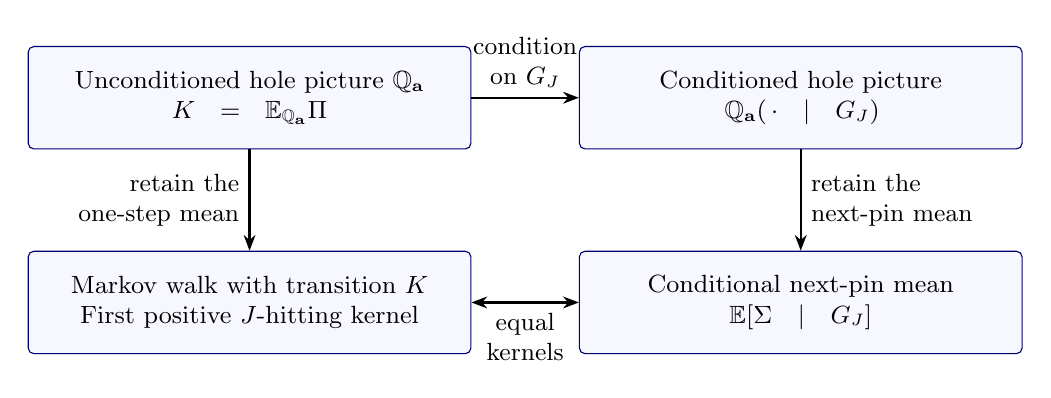
\begin{tikzpicture}[
  box/.style={draw=blue!45!black,rounded corners=2pt,fill=blue!3,
              align=center,text width=5.2cm,minimum height=1.3cm,inner sep=6pt},
  >={Stealth[length=2mm]},font=\small]
  \node[box] (independent) at (0,0)
    {Unconditioned hole picture $\mathbb Q_{\mathbf a}$\\
     $K=\mathbb E_{\mathbb Q_{\mathbf a}}\Pi$};
  \node[box] (conditioned) at (7,0)
    {Conditioned hole picture\\
     $\mathbb Q_{\mathbf a}(\,\cdot\mid G_J)$};
  \node[box] (walk) at (0,-2.6)
    {Markov walk with transition $K$\\
     First positive $J$-hitting kernel};
  \node[box] (moment) at (7,-2.6)
    {Conditional next-pin mean\\
     $\mathbb E[\Sigma\mid G_J]$};
  \draw[->,thick] (independent) -- node[above,align=center]
    {condition\\on $G_J$} (conditioned);
  \draw[->,thick] (independent) -- node[left,align=right]
    {retain the\\one-step mean} (walk);
  \draw[->,thick] (conditioned) -- node[right,align=left]
    {retain the\\next-pin mean} (moment);
  \draw[<->,thick] (walk) -- node[below,align=center]
    {equal\\kernels} (moment);
\end{tikzpicture}
\caption{The first-moment reduction at a fixed exposure and a finite set $J$
of pins on selected time cuts, with $\mathbb Q_{\mathbf a}(G_J)>0$.  The exterior-moment identity is used for the unconditioned
law in the upper-left box; Proposition~\ref{prop:first-moment} proves
that the two routes to the lower-right box agree.  The lower-left walk
resamples its transitions, whereas the upper-right law follows a single
sampled permutation.  The equality concerns the next-pin mean and does
not identify these two path laws.  When the exposure is averaged, its
actual marginal still contains the factor $g_P(\mathbf a)$ in
\eqref{eq:exposure-outer-law}.}
\label{fig:exposure-first-moment}
\end{figure}

\FloatBarrier

\subsection{Fresh turns and continuous boundary pins}

Given an exposure \(\mathbf a\) with \(g_P(\mathbf a)>0\), define
the \emph{fresh-turn walk} on holes as follows.  Repeat periodically the
hole sets, forced transports, and revealed endpoint restrictions.
Between those prescribed changes, the walk jumps across every available
slot edge at rate \(1/2\).  At a forced transport it follows that
transport; at an endpoint completion it uses an independent uniform
completion at the current site.  Use fresh Poisson exchanges and
completion choices in each turn.  These prescriptions define a
time-inhomogeneous Markov walk.  On every bounded time interval it has
finitely many jumps almost surely.  For a starting point \(i\in T\),
write \(\tau_T^+\) for its first strictly positive visit to \(T\),
and \(\tau_E\) for its first visit to \(E\), allowing infinite
hitting times.

\begin{lemma}[Return identity with boundary pins]
\label{lem:exposure-dense-return}
For \(\mathbb P_P\)-almost every exposure and every \(i\in T\),
\begin{equation}
 \mathbb P_P\bigl(\text{next pin after }i\text{ lies in }T
                              \mid\mathcal H\bigr)
   =\mathbb P_{\mathbf a}^{\mathrm{walk}}
                         (\tau_T^+<\tau_E).
 \label{eq:fresh-return-identity}
\end{equation}
In particular the first moment in \eqref{eq:exposure-r} is the
\(\mathbb P_P\)-average of the corresponding fresh-turn return
probabilities in the exposed environment.
\end{lemma}

\begin{proof}
Fix an exposure for which Proposition~\ref{prop:exposure} holds and
\(g_P(\mathbf a)>0\).  Choose increasing finite deterministic time
sets \(\mathcal T_n\) with dense union, and let \(D_{0,n}\) contain
all boundary slots at the times in \(\mathcal T_n\).  Put
\[
 E_n=E_{\mathrm f}\cup D_{0,n},\qquad P_n=E_n\cup T.
\]
The cuts used below include all times occurring in \(P_n\), as well
as time \(0\) if necessary.  An extra unpinned cut merely subdivides
an interval and does not change which cycles hit \(P_n\).

Under \(\mathbb Q_{\mathbf a}\), let \(G_n\) be the event that
all hole cycles meet \(P_n\), and set
\(g_n=\mathbb Q_{\mathbf a}(G_n)\).  The events \(G_n\) increase.
Almost surely the one-period hole picture has only finitely many
random exchanges, in addition to the finitely many prescribed changes.
Its spatial visits have positive residence time: independent Poisson
jumps do not coincide with any prescribed change, and within-site
completions do not change the site.  The exposed histories avoid
\(D_0\), so their cross jumps cannot create an instantaneous
boundary excursion either.  Every boundary visit by a hole cycle is
therefore detected by some cut in the dense union.  There are finitely
many cycles, whence
\begin{equation}
 \1_{G_n}\uparrow\1_{G_P}\quad
       \mathbb Q_{\mathbf a}\text{-almost surely},\qquad
 g_n\uparrow g_P(\mathbf a)>0.
 \label{eq:dense-all-hit-limit}
\end{equation}
In particular, \(g_n>0\) for all sufficiently large \(n\).
No invertibility is required for the earlier indices.

For such an \(n\), Lemma~\ref{lem:exterior} applies to the
unconditioned layered hole permutation.  With \(J=P_n\),
Proposition~\ref{prop:first-moment} identifies each next-pin probability
under \(\mathbb Q_{\mathbf a}(\,\cdot\mid G_n)\) with the
corresponding first-hit probability for its matrix \(K\).  The latter
is precisely the walk just defined, observed at the finitely many cuts:
interval choices are independent, including on later passes through
the same interval.  Thus, if \(A_n\) is the event in a fixed hole
picture that the next \(P_n\)-pin after \(i\) belongs to \(T\),
\begin{equation}
 \frac{\mathbb Q_{\mathbf a}(G_n\cap A_n)}{g_n}
      =\mathbb P_{\mathbf a}^{\mathrm{walk}}
                         (\tau_T^+<\tau_{E_n}).
 \label{eq:finite-cut-return-ratio}
\end{equation}

On the picture side, a cycle through \(i\in T\) returns to \(T\)
after finitely many periods, regardless of which other pins it meets.
Detection of boundary visits before that return shows that
\(\1_{A_n}\) decreases to the event \(A\) that the next full
\(P\)-pin is in \(T\).  Together with
\eqref{eq:dense-all-hit-limit} and bounded convergence, this gives
\[
 \mathbb Q_{\mathbf a}(G_n\cap A_n)
       \longrightarrow\mathbb Q_{\mathbf a}(G_P\cap A).
\]
Dividing by the positive limiting denominator yields the return
probability under \(\mathbb Q_{\mathbf a}(\,\cdot\mid G_P)\).

For the walk side, use a single uncensored fresh-turn trajectory for
all the tests.  Its first positive \(T\)-hitting time \(\tau_T^+\)
is then fixed, independently of \(n\).  The events on the right of
\eqref{eq:finite-cut-return-ratio} decrease.  A path in their
intersection has \(\tau_T^+<\infty\), since this is already part
of each event.  If that path had visited the boundary before
\(\tau_T^+\), the positive residence time of the visit would make
one of the dense cuts detect it before \(\tau_T^+\).  Thus their
intersection is exactly \(\{\tau_T^+<\tau_E\}\), up to a null
set.  Continuity from above gives convergence of the probabilities.
Finally Proposition~\ref{prop:exposure} identifies the limiting
conditional picture law with the conditional law under
\(\mathbb P_P\).  This proves \eqref{eq:fresh-return-identity}.
\end{proof}

\subsection{Minimal hitting probabilities and return energy}

We now ignore all pins of \(E\) except \(D_0\) in the stopping
rule for this walk.  The exposed environment is kept fixed.  This can
only increase its probability of returning to \(T\).  Let
\(U=U(\mathbf a)\) be its one-period column-forward transition
matrix from the cut at \(\theta\) to that same cut one period later,
killed upon every visit to the boundary, including at its initial
point.  Boundary coordinates can be retained with value zero.
With the post-jump convention at deterministic cuts, a period includes
all changes after its starting cut and through its ending cut; in
particular the within-site completion is included exactly once.
All subsequent periods use fresh randomness.

We record the basic contraction property for later heat-flow estimates.
For any subinterval, a realization of all exchanges, forced transports,
and completions gives a bijection between its initial and final hole
sets.  Keeping only trajectories that avoid the boundary gives a
partial permutation: its matrix has at most one entry equal to one
in each row and in each column.  The killed transition matrix \(C\)
is the mean of these matrices.  Hence
\begin{equation}
 C_{ij}\ge0,\qquad
 \sum_i C_{ij}\le1,\qquad \sum_j C_{ij}\le1,
 \qquad \|Cv\|_2\le\|v\|_2.
 \label{eq:hole-contractions}
\end{equation}
Indeed Cauchy--Schwarz in each row gives
\(\sum_i|(Cv)_i|^2\le\sum_{i,j}C_{ij}|v_j|^2
\le\sum_j|v_j|^2\).  The same inequalities apply to adjoints and
to additional killing.  Row sums bound propagated values by one;
column sums bound the total mass from a unit starting point.  These
are statements at a fixed exposure, without any assertion of symmetry
of \(U\) or invariance of the exposure law under time reversal.

\begin{lemma}[Minimal hitting function and return energy]
\label{lem:return-energy}
For almost every exposure under \(\mathbb P_P\), let \(U\) be the
boundary-killed one-period matrix just defined.  There is a smallest
nonnegative function \(f\) on its cut holes satisfying
\begin{equation}
 f=1\text{ on }T,\qquad U^*f=f\text{ off }T.
 \label{eq:minimal-hitting-harmonicity}
\end{equation}
It is given off \(T\) by the probability of ever reaching \(T\)
on a future turn before boundary killing.  In particular
\(0\le f\le1\), and \(f\) is zero on the boundary.  With counting
inner products,
\begin{equation}
 \langle f,(I-U)f\rangle
        =\sum_{i\in T}\bigl(1-(U^*f)_i\bigr),
 \qquad
 m(1-r)\ge
       \mathbb E_P\langle f,(I-U)f\rangle.
 \label{eq:return-energy}
\end{equation}
Both \(U\) and \(f\) in this expectation are functions of the same
exposure, with the outer law in \eqref{eq:exposure-outer-law}.
\end{lemma}

\begin{proof}
Set \(f_0=\1_T\) and recursively define
\begin{equation}
 f_{n+1}=\1_T+\1_{H_\theta\setminus T}\,U^*f_n,
 \label{eq:finite-horizon-hitting}
\end{equation}
where the multiplication by the indicator is pointwise.
Nonnegativity and the substochasticity of \(U^*\) show inductively
that \(0\le f_n\le f_{n+1}\le1\).  The Markov property identifies
\(f_n\), off \(T\), with the probability of reaching \(T\)
within the next \(n\) periods before killing.  Thus its pointwise
limit \(f\) has the asserted probability interpretation.  There are
finitely many coordinates, so passage to the limit in
\eqref{eq:finite-horizon-hitting} gives
\eqref{eq:minimal-hitting-harmonicity}.  A boundary starting point is
killed immediately, and consequently every \(f_n\) and \(f\) is
zero there.

If \(h\) is any nonnegative solution of
\eqref{eq:minimal-hitting-harmonicity}, then \(h\ge f_0\) and
induction in \eqref{eq:finite-horizon-hitting} gives \(h\ge f_n\)
for every \(n\); hence \(h\ge f\).  This proves minimality.
In particular \(f\) is zero on any closed class that cannot reach
\(T\).  No assumption of certain absorption by the boundary is
needed.

Since \(T\) occurs at a single time modulo the period, a strictly
positive return from that cut to \(T\) occurs after an integer number
of periods.  Conditioning on the first period therefore shows that
the relaxed return probability from \(i\in T\) is \((U^*f)_i\).
By Lemma~\ref{lem:exposure-dense-return}, the conditional probability
\(q_i(\mathbf a)\) contributing to \eqref{eq:exposure-r} is the
return probability with all of \(E\) retained.  Hence
\[
 q_i(\mathbf a)\le (U^*f)_i\qquad(i\in T).
\]
The vectors are real, so transposition in the scalar quadratic form
and harmonicity off \(T\) give
\begin{align*}
 \langle f,(I-U)f\rangle
   &=\langle (I-U^*)f,f\rangle\\
   &=\sum_{i\in T}\bigl(1-(U^*f)_i\bigr)
    \le\sum_{i\in T}(1-q_i(\mathbf a)).
\end{align*}
Averaging under the actual exposure marginal gives
\eqref{eq:return-energy}.  Measurability causes no additional
limiting issue: finite-time transition probabilities are measurable
functions of the finite-jump exposure, and \(f\) is the increasing
limit of the finite-horizon functions in
\eqref{eq:finite-horizon-hitting}.
\end{proof}

For the estimates that follow, write \(\eta=\1_T\) and \(g=f-\eta\).
Then \(0\le g\le1\), \(\langle\eta,g\rangle=0\), and both
functions have zero boundary values.  Lemma~\ref{lem:return-energy}
shows that the desired scale of quadratic loss is \(m\): for any
\(\varepsilon\ge0\),
\[
 \mathbb E_P\langle f,(I-U)f\rangle\ge m(1-\varepsilon)
 \quad\Longrightarrow\quad r\le\varepsilon.
\]
The simultaneous pin test then bounds the old-pin avoidance probability
by \((2\varepsilon)^m\).  The next sections obtain this lower bound
with a small error from the spatial distribution of holes and the
corresponding heat flow.

\section{Sparse obstacles and local diffusion}\label{sec:sparse}

The return-energy problem requires two spatial estimates in each exposed
environment.  Mass initially on $T$ must spread through nearby holes,
and its pairing, after propagation, with the remainder $g=f-\1_T$ of
the hitting function must be bounded by the energy of that propagated
remainder.
Short connections near each starting point supply the first estimate;
flows through the rest of the lattice will supply the second.
We now derive the geometric conditions for both from the sparse pin-test
induction.  This section bounds the probability that these conditions
fail and proves the local Nash inequality.
Section~\ref{sec:flows} constructs the flows, and
Section~\ref{sec:leakage} uses both estimates to close the induction.

\subsection{The induction input and blocking between cuts}

Fix throughout
\begin{equation}\label{eq:sparse-exponents}
 \alpha=\frac1{100},\qquad \nu=\frac1{100d},\qquad a=\frac{11}{10}.
\end{equation}
All spatial distances in this and the following two sections are in the
supremum norm, and
\(B_h(x)=\{z\in\Z^d:|z-x|_\infty\le h\}\).
A finite collection of slot points with spatial coordinates \((x_i)_{i\in A}\)
is called \emph{sparse} if
\begin{equation}\label{eq:sparse-growth}
 \#\{i\in A:x_i\in B_h(z)\}\le L(1+h)^\alpha
 \qquad(z\in\Z^d,\ h\ge0).
\end{equation}
Repeated spatial coordinates are counted with their slot multiplicities.
The constant \(L\ge\max\{2d,\ell,4\}\) is fixed independently of all scales.
For a set of distinct sites, sparseness means the same inequality with one
point per site.  Every subset of a sparse collection is sparse.

Let \(0<p<1\), put
\begin{equation}\label{eq:sparse-scales}
 s=p^{-a},\qquad R=\lceil C_*s\rceil,
 \qquad \beta\ge5s,
\end{equation}
and choose a finite circular time grid \(\mathcal G\subset\R/\beta\Z\)
containing \(0\), whose successive gaps are at most \(p^{4d}\).
Here \(C_*\ge1\) is a fixed constant, to be chosen for the localization
estimate.  Write \(\mathcal V_{\mathcal G}=V_\Lambda\times\mathcal G\).
For \(D=D_0\cup F\), where \(F\subseteq\mathcal V_{\mathcal G}\), let
\(\mathsf I_p(D)\) denote the assertion
\begin{equation}\label{eq:induction-assertion}
 \mathbb P_D(A\subseteq\mathcal B_D)\le p^{|A|}
 \quad\text{for every nonempty sparse set }A\subseteq
 \mathcal V_{\mathcal G}\setminus D
 \text{ at a single grid time}.
\end{equation}
There are only finitely many grid points outside \(D_0\).
Thus one may prove these assertions by downward induction on the number
of pins, starting from the vacuous assertion when every grid point is
pinned.  In a step with pin set \(E\) and test \(T\), the set
\(P=E\cup T\) has strictly more pins.  In the present section we assume
\(\mathsf I_p(P)\); we do not assume \(\mathsf I_p(E)\).
Under this hypothesis we will seek a bound
\(r(E,T)\le\varepsilon(p)\) with \(\varepsilon(p)=o(p)\).
Proposition~\ref{prop:pin-test} then yields the required
\(p^{|T|}\) bound for the test under \(\mathbb P_E\), once
\(2\varepsilon(p)\le p\).

Expose \(\mathcal B_P\) under \(\mathbb P_P\) as in
Proposition~\ref{prop:exposure}.  A site is \emph{blocked} at time \(t\)
if none of its \(\ell\) slots is a hole.  Denote the blocked set by
\(\mathcal O_t\).  Extend the environment to \(\Z^d\) by making all
slots outside \(\Lambda\) available.  Boundary sites also have all slots
available because \(D_0\subseteq P\).  In particular \(\mathcal O_t\)
is finite and is disjoint from the inner boundary.

Sparse growth serves two purposes.  A blocked path crossing a large
spatial scale will supply a separated collection satisfying
\eqref{eq:sparse-growth}, so the restricted induction hypothesis can
still detect large obstacles.  Later, the same growth bound on the
test points will make overlaps between their decaying flows summable.
The component estimate below and the energy estimate in
Proposition~\ref{prop:flow-energy} implement these two uses.

At a grid time \(q\), the induction input gives
\begin{equation}\label{eq:grid-blocking}
 \mathbb P_P(A\subseteq\mathcal O_q)\le p^{|A|}
 \qquad\text{for every prescribed sparse set of distinct sites }A.
\end{equation}
Indeed, choose one fixed slot at each site.  If any chosen slot is pinned,
or any site is outside the volume, blocking is impossible.  Otherwise the
chosen slot points form an admissible test in \(\mathsf I_p(P)\).

\begin{lemma}[Blocking at a deterministic time]\label{lem:nongrid}
Assume \(\mathsf I_p(P)\), and let \(t\) be any deterministic time.
There is a constant \(C_0=C_0(d,\ell)\), uniform in \(p\le1\), the
volume, the period, the grid, and \(P\), such that, for every prescribed
finite set \(A\subset\Z^d\) of distinct sites,
\begin{align}
 \mathbb P_P(A\subseteq\mathcal O_t)&\le C_0p^{2d}
 &&\text{if }|A|=2d,                                      \label{eq:small-blocking}\\
 \mathbb P_P(A\subseteq\mathcal O_t)&\le(C_0\sqrt p)^{|A|}
 &&\text{if }A\text{ is a nonempty sparse set of distinct sites}.
                                                               \label{eq:sparse-blocking}
\end{align}
\end{lemma}

\begin{proof}
Let \(q\) be the preceding grid time and \(I=(q,t]\), interpreted
cyclically, so that \(|I|\le p^{4d}\).  On-site permutations do not
change the number of holes at a site.  Consequently a site blocked at
\(t\) was either blocked at \(q\) or has an incident inter-site mark
in \(I\).  This remains true when \(I\) crosses the time seam.
By Lemma~\ref{lem:factorial}, the expected number of marks in the
edge star of a prescribed site during \(I\) is at most
\(2d\ell^2|I|\).
If all \(2d\) prescribed sites are blocked at \(t\), either they were
all blocked at \(q\), or one of these finitely many edge stars contains
a mark.  Their set is sparse since \(L\ge2d\).  The union bound and
\eqref{eq:grid-blocking} give
\(p^{2d}+C p^{4d}\le Cp^{2d}\).

Now let \(n=|A|\) and assume \(A\) is sparse.  If every site of \(A\)
is blocked at \(t\), either at least \(\lceil n/2\rceil\) of its sites
were blocked at \(q\), or at least \(\lceil n/2\rceil\) have an
incident mark in \(I\).  For the first alternative, summing
\eqref{eq:grid-blocking} over subsets costs at most
\(2^n p^{\lceil n/2\rceil}\).
For the second, one of the two lattice parities supplies at least
\(k=\lceil n/4\rceil\) sites with incident marks.  Edge stars of
distinct sites of the same parity are disjoint.  If \(N_z\) counts
marks in the star of \(z\) during \(I\), then for any such prescribed
\(k\)-set \(A'\), the product \(\prod_{z\in A'}N_z\) counts
choices of \(k\) distinct marks.  The factorial bound therefore yields
\[
 \mathbb P_P(N_z\ge1\text{ for all }z\in A')
 \le \mathbb E_P\prod_{z\in A'}N_z
 \le (2d\ell^2|I|)^k.
\]
Summing over at most \(2^{n+1}\) possible choices bounds the second
alternative by \(2^{n+1}(C p^{4d})^{\lceil n/4\rceil}\).
As \(4d\lceil n/4\rceil\ge dn\ge n/2\), both alternatives are
bounded together by \((C_0\sqrt p)^n\), after enlarging \(C_0\).
These are separate event bounds combined by a union bound; no
independence between old blocking and intervening marks is required.
\end{proof}

\subsection{Admissible binary witnesses and component tails}

Join two blocked sites when their supremum distance is at most \(8\).
All components and paths of blocked sites below use this adjacency.
For \(z\in\mathcal O_t\), let \(\mathcal C_t(z)\) be its component
and set
\[
 \operatorname{rad}_z\mathcal C_t(z)
 =\max_{w\in\mathcal C_t(z)}|w-z|_\infty.
\]
The next lemma gives a tail uniform even as the bootstrap parameter is
subsequently decreased.

\begin{lemma}[Uniform component tail]\label{lem:component-tail}
There are \(p_0>0\) and \(c,C,\gamma>0\), depending only on
\(d,\ell\) and the fixed sparse-growth choices, such that whenever
\(0<p\le p_0\) and \(\mathsf I_p(P)\) holds,
\begin{equation}\label{eq:component-tail}
 \mathbb P_P\bigl(z\in\mathcal O_t,\
      \operatorname{rad}_z\mathcal C_t(z)\ge h\bigr)
 \le C\exp(-ch^\gamma)
 \qquad(z\in\Z^d,\ h\ge1)
\end{equation}
at every deterministic time \(t\).  The constants \(c,C,\gamma\)
are fixed once \(p_0\) is fixed and work simultaneously for all
\(p\le p_0\).
\end{lemma}

\begin{proof}
Fix an integer \(b>100\) so large that \(b^\alpha>4\), and put
\(h_j=16b^j\).  We first describe exactly which site lists will be
used as witnesses.  Their separated binary-tree structure is also used
in multiscale cascading-event arguments; see, for example,
\cite[Section~3]{Sznitman2012}.  Here the leaf probabilities will come
directly from \eqref{eq:sparse-blocking}.  A depth-\(j\) witness rooted at \(z\) is an
assignment of sites \(x_w\) to the vertices \(w\) of a rooted ordered
binary tree of depth \(j\), with \(x_\varnothing=z\).  If a vertex
\(w\) has \(k\ge1\) levels below it, require
\begin{equation}\label{eq:witness-admissibility}
 x_{w0}=x_w,\qquad x_{w1}\in B_{h_k+8}(x_w),\qquad
 \operatorname{dist}_\infty(\mathcal L_{w0},\mathcal L_{w1})
       \ge h_k/4,
\end{equation}
where \(\mathcal L_{wa}\) is the set of leaf sites descended from
child \(wa\).  Call such an assignment \emph{admissible}.
Its leaves are distinct by the separation condition.  Depth zero has
just the prescribed root as its leaf.

A blocked crossing from \(z\) to distance at least \(h_j\) produces
an admissible witness all of whose leaves are blocked.  For \(j=0\)
use the root alone.  For \(j\ge1\), truncate the crossing at its
first exit to distance \(h_j\); it is
contained in \(B_{h_j+8}(z)\).  One child crossing starts at \(z\).
The other starts at the first site whose distance from \(z\) is at
least \(h_j/2\), hence at distance at most \(h_j/2+8\).
The remaining part of the parent crossing reaches distance at least
\(h_j/2-8\) from this second start.  Each child can thus be truncated
at its first exit to distance \(h_{j-1}\), and is contained in its
start-centered ball of radius \(h_{j-1}+8\).  The distance between
these two balls is at least
\[
 h_j/2-2(h_{j-1}+8)\ge h_j/4.
\]
Recurse on the two truncated child crossings.  Every descendant leaf
remains in its child's truncated crossing, so all the separation
conditions in \eqref{eq:witness-admissibility} hold.

Every admissible witness has a sparse leaf set.  Indeed, for
\(1\le k\le j\), a ball of diameter strictly less than \(h_k/4\)
meets at most one child at every split of scale at least \(h_k\).
It therefore contains at most \(2^{k-1}\) leaves.  If
\(h_{k-1}/8\le h<h_k/8\), this bound is at most
\(L(1+h)^\alpha\), since
\[
 L(1+h)^\alpha\ge L(2b^{k-1})^\alpha
       \ge 2^{k-1}.
\]
For \(h<h_0/8\) there is at most one leaf, and for
\(h\ge h_j/8\) the same calculation allows all \(2^j\) leaves.
The depth-zero case is immediate.  This verifies
\eqref{eq:sparse-growth} for all centers and real radii, including
the scale endpoints.

Let \(A_j\) be an upper bound on the number of admissible assignments
rooted at any prescribed site.  At the top split the first child root
is fixed and the second has at most \((C_dh_j)^d\) choices.
Ignoring restrictions between the two child assignments gives the
numerical overcount
\[
 A_0=1,\qquad A_j\le(C_dh_j)^d A_{j-1}^2.
\]
In particular
\[
 2^{-j}\log A_j
 \le d\sum_{k=1}^j2^{-k}\log(C_dh_k)
 \le \log C_b<\infty,
 \qquad A_j\le C_b^{2^j}.
\]
Only admissible assignments enter the probability union bound.  The
unrestricted product used to bound their number need not itself
consist of sparse witnesses.

For each admissible assignment, Lemma~\ref{lem:nongrid} bounds the
probability that all its leaves are blocked by
\((C_0\sqrt p)^{2^j}\).  Choose \(p_0\le1\) once and for all so
that \(C_bC_0\sqrt{p_0}\le e^{-2}\).  For every \(p\le p_0\),
\begin{equation}\label{eq:discrete-component-tail}
 \mathbb P_P\bigl(z\in\mathcal O_t,\
      \operatorname{rad}_z\mathcal C_t(z)\ge h_j\bigr)
 \le \exp(-2\cdot2^j).
\end{equation}
For \(h\ge16\), choose \(j\ge0\) with
\(h_j\le h<h_{j+1}\).  Then
\(2^j\ge(h/(16b))^\gamma\), where \(\gamma=\log_b2>0\).
This proves \eqref{eq:component-tail}; increasing \(C\) covers
\(1\le h<16\).  No constant in this last step changes when \(p\)
is decreased further.
\end{proof}

\subsection{Regular anchors}

We now separate the geometry near the starting point of a localized
mass from the geometry farther away.  Nearby, fewer than $2d$ blocked
sites in each fixed-radius ball will preserve short lattice connections;
these connections transfer the lattice Nash inequality to the holes.
Farther away, a sublinear bound on component radii will control the
displacement of the routes used for flows to infinity in
Section~\ref{sec:flows}.  The first condition gives local diffusion,
and the second permits the global energy comparison.
Let \(M_*\) be a fixed positive integer.  Its required size will be
specified below, independently of \(p\).

\begin{definition}[Regular anchor]\label{def:regular-anchor}
For a spatial anchor \(x\in\Z^d\), call time \(t\)
\emph{regular for \(x\)} at scale \(R\) if both conditions hold:
\begin{enumerate}
 \item For every \(z\in B_{11R}(x)\),
       \(\#(\mathcal O_t\cap B_{M_*}(z))<2d\).
 \item For every \(z\in\mathcal O_t\setminus B_{10R}(x)\),
       \(\operatorname{rad}_z\mathcal C_t(z)
            \le(1+|z-x|_\infty)^\nu\).
\end{enumerate}
For \(i\in T\), ``regular for \(i\)'' means regular for its spatial
coordinate \(x_i\).
\end{definition}

\begin{proposition}[Probability of irregularity]\label{prop:regularity}
Fix \(M_*\).  Under \(\mathsf I_p(P)\), for all \(0<p\le p_0\),
all deterministic times \(t\), and all spatial anchors \(x\),
\begin{equation}\label{eq:regularity-failure}
 \mathbb P_P(t\text{ is not regular for }x)
 \le \delta:=C R^d p^{2d}+C\exp(-cR^\xi),
 \qquad \xi=\nu\gamma>0.
\end{equation}
Here \(R\ge1\), and the constants may depend on \(M_*\) but are
uniform in \(p\le p_0\), volume, period, grid, pin set and anchor.
\end{proposition}

\begin{proof}
There are at most \(C R^d\) centers in \(B_{11R}(x)\), and a ball
of radius \(M_*\) has a fixed number of \(2d\)-element subsets.
The union bound and \eqref{eq:small-blocking} therefore bound failure
of the first condition by \(C R^d p^{2d}\).
By Lemma~\ref{lem:component-tail}, failure of the second has probability
at most
\[
 C\sum_{z:|z-x|_\infty>10R}
   \exp\bigl(-c(1+|z-x|_\infty)^{\nu\gamma}\bigr)
 \le C\exp(-c'R^{\nu\gamma}).
\]
For the last inequality, count at most \(C(1+n)^{d-1}\) sites at
distance \(n\) and absorb this polynomial and the tail summation
into half of the exponential.  Since \(\nu\gamma>0\) is fixed,
the resulting constants are uniform.  Add the two bounds.
\end{proof}

We will use \eqref{eq:regularity-failure} only at prescribed times and
after integration in time.  It asserts neither independence between
slices nor regularity simultaneously at every time.

\subsection{Local connections and the Nash inequality}

The remaining statements in this section are deterministic.  At a
fixed time let \(\mathcal H_t\) be the graph whose vertices are the
available slots on the extended lattice and whose edges join every
pair of available slots above nearest-neighbor sites.  For a real
function \(v\) on its vertices define
\begin{equation}\label{eq:slot-energy}
 \mathcal D_t(v)=\frac12
 \sum_{\{i,j\}\in E(\mathcal H_t)}(v_i-v_j)^2.
\end{equation}
Edges in this sum are unoriented and counted once.  Norms use counting
measure on the available slots.  When a function describes killed
mass, its values at the physical boundary and outside the volume are
zero.  Thus \eqref{eq:slot-energy} includes the edges into the
zero-valued boundary, as required by Dirichlet killing.

\begin{lemma}[Uniform local connectivity]\label{lem:local-connectivity}
Let \(d\ge2\) and \(K\ge1\) be fixed.  There is an integer
\(\rho=\rho(d,K)\ge K+1\) such that the following holds.
If \(u,v\in\Z^d\), \(|u-v|_\infty\le K\), and
\(F\subset\Z^d\) satisfies
\[
 u,v\notin F,\qquad \#(F\cap B_\rho(u))<2d,
\]
then a nearest-neighbor path from \(u\) to \(v\) avoids \(F\),
lies in \(B_\rho(u)\), and has length at most \((2\rho+1)^d\).
\end{lemma}

\begin{proof}
First suppose \(F\) is a set of fewer than \(2d\) sites in the
whole lattice.  The complement of a box containing \(F\) is connected
when \(d\ge2\), so \(\Z^d\setminus F\) has only one possible
infinite component.  It has no finite component: from a vertex of
such a component the first exit along each of the \(2d\) positive
and negative coordinate rays must lie in \(F\), giving \(2d\)
distinct deleted sites.  Hence \(\Z^d\setminus F\) is connected.

The confinement radius can be uniform when the two endpoints have
bounded separation.  Otherwise, after translating the first endpoint
to \(0\), there would be sets \(F_n\) with \(|F_n|<2d\) and
surviving endpoints \(v_n\in B_K(0)\), admitting no path inside
\(B_n(0)\).  Pass to a subsequence with \(v_n=v\) and with the
indicators of \(F_n\) converging pointwise on \(\Z^d\).  The limiting
set \(F_\infty\) has fewer than \(2d\) sites and avoids both
endpoints.  By the preceding paragraph there is a finite path from
\(0\) to \(v\) avoiding \(F_\infty\).  For all sufficiently large
\(n\), this path lies in \(B_n(0)\) and avoids \(F_n\), a
contradiction.  Choose a uniform radius \(\rho\ge K+1\).

For the asserted local version apply this conclusion to
\(F'=F\cap B_\rho(u)\), a set of fewer than \(2d\) sites in the
whole lattice.  The resulting path lies in \(B_\rho(u)\), where
\(F'\) and \(F\) agree.  Erasing loops gives the claimed length bound.
\end{proof}

We may now make the local radius choice without reference to \(p\).
Fix
\begin{equation}\label{eq:local-radius-choice}
 K_{\mathrm{conn}}=8(2d-2)+12,\qquad
 M_*\ge\max\{8(2d),\rho(d,K_{\mathrm{conn}})+2\}.
\end{equation}
We henceforth require \(R\) to exceed these fixed local radii, which
is achieved by decreasing the final \(p\).  At a regular anchor,
Lemma~\ref{lem:local-connectivity} is now available for surviving
sites within separation \(K_{\mathrm{conn}}\), whenever its first
endpoint lies in \(B_{11R}(x)\).  In particular, it applies to every
short connection used below.  This choice also serves the local
source connections in Section~\ref{sec:flows}.

The next estimate uses Nash's norm--energy inequality and its diffusion
mechanism~\cite[Part~I]{Nash1958}.  The transfer to the available slots
uses path comparison of Dirichlet forms, a method developed
systematically by Diaconis and Saloff-Coste
\cite[Theorem~2.1]{DiaconisSaloffCoste1993}.  We supply the comparison
for the present obstacles and zero extension explicitly.

\begin{proposition}[Local Nash inequality]\label{prop:local-nash}
Fix \(d\ge3\), \(\ell\), and \(M_*\) as in
\eqref{eq:local-radius-choice}.  Let \(\mathcal H_t\) be an available-slot
graph with at least one and at most \(\ell\) slots at every unblocked
site, and suppose \(t\) is regular for \(x\) at scale
\(R\ge M_*+K_{\mathrm{conn}}+3\).
Every nonnegative function \(v\) supported on slots above \(B_R(x)\)
satisfies
\begin{equation}\label{eq:local-nash}
 \|v\|_2^{2+4/d}\le C\mathcal D_t(v)\|v\|_1^{4/d},
\end{equation}
where \(C\) depends only on \(d,\ell\) and the fixed local radii.
\end{proposition}

\begin{proof}
We transfer \(v\) to a lattice function while controlling energy, then
prove the lattice inequality by averaging.  At every surviving site
\(z\), choose an available slot maximizing \(v\), and let \(V(z)\)
be this maximum.  Every blocked site in \(B_{R+3}(x)\) has a surviving
nearest neighbor: otherwise its \(2d\) neighbors alone would violate
the first regularity condition in the ball centered there.  Choose
one such neighbor \(\phi(z)\) and define
\[
 w(z)=
 \begin{cases}
   V(z),&z\notin\mathcal O_t,\\
   V(\phi(z)),&z\in\mathcal O_t\cap B_{R+3}(x),\\
   0,&z\in\mathcal O_t\setminus B_{R+3}(x).
 \end{cases}
\]
The function \(w\) is supported in \(B_{R+1}(x)\).  Since a site's
value is copied only by its nearest neighbors,
\begin{equation}\label{eq:nash-norm-transfer}
 \|v\|_2^2\le\ell\|w\|_2^2,
 \qquad \|w\|_1\le(2d+1)\|v\|_1.
\end{equation}

For a lattice edge \(\{z,z'\}\) with a nonzero endpoint value,
both endpoints belong to \(B_{R+2}(x)\).  Each of \(w(z),w(z')\)
is the value at a chosen maximizing slot over a surviving site,
say \(u,u'\), at distance at most one from the corresponding
endpoint.  Thus \(|u-u'|_\infty\le3\) and \(u,u'\in B_{R+3}(x)\).
Lemma~\ref{lem:local-connectivity} joins them through surviving sites
within a fixed radius of \(u\), with a fixed length bound.  Lift
this path using the chosen maximizing slot at every site.  Every
lifted edge is available because all pairs of available slots across
a lattice edge are joined.  If \(u=u'\), the difference is zero.
Otherwise telescoping and Cauchy--Schwarz show that
\((w(z)-w(z'))^2\) is at most a fixed constant times the sum of
\((v_i-v_j)^2\) along the lifted path.
For any fixed slot edge, only a bounded number of the original
lattice edges can have a path using it: all of their endpoints lie
within a fixed radius of that edge.  Hence, summing,
\begin{equation}\label{eq:nash-energy-transfer}
 \sum_{\{z,z'\}:|z-z'|_1=1}(w(z)-w(z'))^2
 \le C\mathcal D_t(v).
\end{equation}

For completeness, write \(\mathcal E_{\Z^d}(w)\) for the sum on
the left of \eqref{eq:nash-energy-transfer}.  For an integer
\(k\ge1\), let \(A_kw\) be the average of translates of \(w\)
by the points of \(\{0,\ldots,k-1\}^d\).  Telescoping a translate
along coordinate directions, followed by Cauchy--Schwarz, gives
\[
 \|w-A_kw\|_2^2\le C_d k^2\mathcal E_{\Z^d}(w).
\]
The averaging kernel has counting \(2\)-norm \(k^{-d/2}\);
the convolution inequality therefore gives
\(\|A_kw\|_2^2\le k^{-d}\|w\|_1^2\).  Consequently
\[
 \|w\|_2^2\le C_d k^2\mathcal E_{\Z^d}(w)
                 +2k^{-d}\|w\|_1^2.
\]
If \(w\ne0\), choose
\(k=\lceil(4\|w\|_1^2/\|w\|_2^2)^{1/d}\rceil\).
The second term is at most \(\|w\|_2^2/2\), and
\(\|w\|_1^2/\|w\|_2^2\ge1\) bounds the effect of rounding.
Absorption yields
\[
 \|w\|_2^{2+4/d}
 \le C_d\mathcal E_{\Z^d}(w)\|w\|_1^{4/d}.
\]
For \(w=0\) the inequality is immediate.  Finally use
\eqref{eq:nash-norm-transfer} and \eqref{eq:nash-energy-transfer}
to obtain \eqref{eq:local-nash}.
\end{proof}

The order of choices is now explicit.  First fix \(d,\ell\), the
exponents in \eqref{eq:sparse-exponents}, the witness scale ratio
\(b\), and \(L\).  Next fix the preliminary \(p_0\) and the uniform
tail constants in Lemma~\ref{lem:component-tail}.  Fix the connectivity
radii and \(M_*\) by \eqref{eq:local-radius-choice}; this fixes the
constants in Proposition~\ref{prop:regularity} and
Proposition~\ref{prop:local-nash}.  Choose \(C_*\) for localization,
and only then decrease \(p\le p_0\) so that \(R\) exceeds the fixed
radii and the leakage error is small enough to close the induction.
Thus no tail constant deteriorates as the final \(p\) is decreased.
The next section uses the same regularity conditions to construct
flows to infinity, complementing the local diffusion bound proved here.

\section{Flows around the blocked components}\label{sec:flows}

Fix one time slice $t$.  The graph $\mathcal H_t$ consists of the available slots, including
all $\ell$ slots at every site outside $\Lambda$, with all available slot
pairs across each nearest-neighbor site edge.  Write $\mathcal Z=\mathcal O_t$
for its finite blocked set.  We will represent masses near regular anchors as divergences
of flows with controlled energy.  This will bound their pairing with a
function by that function's Dirichlet energy, the estimate needed for the
cross term in Section~\ref{sec:leakage}.
The divergence and energy viewpoint is the classical electrical-network
flow method; see \cite[Sections~1.3.5 and~2.4.6]{DoyleSnell1984}.
The geometric work here is to retain a quantitative decay bound after
routing through this dependent obstacle configuration.

Give every unoriented slot edge $e$ a reference orientation $(e^-,e^+)$.
A flow is a real function $J$ on these reference edges; its divergence is
outgoing minus incoming flow.  Thus a signed unit path from $a$ to $b$
has divergence $\1_{\{a\}}-\1_{\{b\}}$.  Write
$\dist(e,y)=\min\{|x-y|_\infty:x\text{ is an endpoint site of }e\}$.
Constants in this Section depend only on $d,\ell$ and the fixed geometric
constants in Section~\ref{sec:sparse}, never on the slice or volume.

The construction begins with a full-lattice unit flow whose strength at
distance $h$ from its source is $O((1+h)^{1-d})$.  We replace each oriented
lattice edge by a path through available slots, with endpoints given by
one application of a map on the original vertices.  A short additional
path then restores the source at the specified slot.  The geometry below
bounds the displacement of the replacement paths, and hence the number
of original edges that can contribute to a given available edge.
The resulting decay will let us add flows from a sparse collection of
sources with controlled total energy.

\subsection{Filled hulls and their surviving boundaries}

We first thicken each blocked component to obtain clearance for routes
around it.  After filling the finite pockets of its complement, we will
show that the exterior vertex boundary is connected by sup-norm steps of
length at most one.  These steps can be replaced by unblocked
nearest-neighbor paths.  The filled sets may be nested; their
inclusion-maximal members will give disjoint regions on which to define
the vertex map.

Let $C$ range over the components of $\mathcal Z$ for steps of sup norm
at most eight.  Set
\[
 A_C=\{z\in\Z^d:\dist(z,C)\le4\},\qquad
 H_C=\Z^d\setminus U_C,
\]
where $U_C$ is the infinite nearest-neighbor component of
$\Z^d\setminus A_C$.  Such an infinite component is unique: the exterior
of a box containing $A_C$ is connected when $d\ge2$.  Thus $H_C$ is
$A_C$ with its finite complementary components filled in.  The exterior
vertex boundary of $H_C$ is
\[
 S_C=\{v\notin H_C:\text{some }u\in H_C\text{ satisfies }|u-v|_1=1\}.
\]

The exterior-boundary connectivity in the next lemma is the lattice case
of Tim\'ar's boundary-connectivity result~\cite[Lemmas~1--2]{Timar2013}.
We include the plaquette proof together with the separate hull and
clearance estimates needed for the routes.

\begin{lemma}[Hull topology and clearance]\label{lem:hulls}
Let $d\ge2$ and let $\mathcal Z\subset\Z^d$ be finite.  The sets $A_C$
are pairwise disjoint and nearest-neighbor connected.  Each $H_C$ is finite,
is nearest-neighbor connected, has connected complement, and is contained
in the coordinate bounding box of $A_C$.  Any two hulls are disjoint or one
contains the other.

For every edge $\{u,v\}$ with $u\in H_C$, $v\notin H_C$,
\begin{equation}\label{eq:hull-clearance}
 \dist(u,C)=4,\qquad \dist(v,C)=5.
\end{equation}
Both endpoints are unblocked.  The set $S_C$ is connected by steps of sup
norm at most one.  Each such step can be replaced by a nearest-neighbor
path of unblocked sites, contained in the unit enlargement of the bounding
box of $A_C$.  Consequently any two points of $S_C$ can be joined by a
finite path of unblocked sites in that enlargement.
\end{lemma}

\begin{proof}
Distinct components have mutual distance at least nine, so their
radius-four thickenings are disjoint.  The radius-four lattice cubes about
successive points of a component intersect; their union is connected.
Every finite complementary component has a neighbor in $A_C$, which proves
that filling preserves connectivity.  A vertex outside the coordinate
bounding box has a coordinate ray avoiding that box, so it belongs to
$U_C$.  This proves finiteness and the claimed containment.

For laminarity, take two disjoint connected thickenings $A_C,A_{C'}$.
The second lies in a single component of the complement of the first.
If it lies in a finite component, then $U_C$ is an infinite connected
subset of the complement of $A_{C'}$, whence $U_C\subset U_{C'}$ and
$H_{C'}\subset H_C$.  The reversed containment is treated identically.
In the remaining case each thickening lies in the infinite complementary
component of the other.  Then $H_C$ avoids $A_{C'}$ and is connected;
since it contains $A_C\subset U_{C'}$, it lies wholly in $U_{C'}$.
Hence $H_C$ and $H_{C'}$ are disjoint.

We next prove connectivity of the exterior boundary without a planar
separation argument.  Let $\mathcal E_C$ be the edges between $H_C$ and
$U_C$, and join two of these edges when they lie on an elementary lattice
plaquette.  Every plaquette meets $\mathcal E_C$ an even number of times,
and all cut edges of one plaquette belong to the same component of this
edge relation.  Thus each component separately meets every plaquette
evenly.  It then meets every finite closed lattice walk evenly: modulo two,
such a walk is a sum of elementary plaquettes, as follows by commuting
successive steps in different coordinate directions and canceling inverse
steps.  If the cut had two components, take one edge from each, join their
inner endpoints within $H_C$ and their outer endpoints within $U_C$.
The resulting closed walk uses exactly one cut edge from each chosen
component, a contradiction.  The cut is therefore connected by plaquettes.
The outer endpoints of cut edges on a common plaquette have sup distance
at most one.  This proves the asserted connectivity of $S_C$.

An inner cut endpoint $u$ must belong to $A_C$: otherwise a complementary
pocket containing $u$ would be adjacent to the infinite component through
$v$, which is impossible.  Since $v\notin A_C$ and $|u-v|_\infty=1$,
the distances to $C$ are exactly four and five.  For another component
$C'$, separation gives $\dist(v,C')\ge4$ and $\dist(u,C')\ge5$.
To interpolate a sup step between two points of $S_C$, change the differing
coordinates one at a time.  Every intermediate vertex is within sup
distance one of its starting point, hence has distance at least four
from $C$ and at least three from every other component.  All these
vertices survive.  They also remain in the coordinate bounding box of
$S_C$, which is contained in the unit enlargement stated above.
\end{proof}

Keep only the inclusion-maximal hulls and denote their family by
$\mathfrak H$.  They are pairwise disjoint and contain all blocked sites.
Choose one representative $r_H\in S_C$ for each $H=H_C\in\mathfrak H$,
and define a map on sites by
\begin{equation}\label{eq:once-only-map}
 \rho(z)=
 \begin{cases}
 r_H,&z\in H\in\mathfrak H,\\
 z,&z\notin\bigcup_{H\in\mathfrak H}H.
 \end{cases}
\end{equation}
All images are unblocked.  The map is applied once.  A representative
can lie in another hull, so no identity $\rho(r_H)=r_H$ is assumed.

For each oriented lattice edge $(u,v)$, join $\rho(u)$ to $\rho(v)$ as
follows.  If both endpoints are in the same hull, use the empty path.
If neither is in a hull, use the edge itself.  If only $u$ belongs to a
hull $H$, then $v\in S_C$ and a path along its surviving boundary joins
$r_H$ to $v$; reverse this prescription when only $v$ is in a hull.
Finally, if $u\in H$ and $v\in H'$ for distinct maximal hulls, both
$u$ and $v$ survive and the signed route is
\begin{equation}\label{eq:adjacent-hull-route}
 r_H\ \longrightarrow\ v\ \longrightarrow\ u\ \longrightarrow\ r_{H'}.
\end{equation}
The first portion uses the exterior boundary of $H$, the last the exterior
boundary of $H'$, and the middle portion traverses the original edge in
reverse.  Indeed $v\in S_C$ and $u\in S_{C'}$.  Erase loops from the
resulting walk, leaving a simple path with the same endpoints.  This path
stays in the enlarged bounding boxes of the hulls incident to the original
edge, together with that edge.  Figure~\ref{fig:hull-routing} shows an
exterior-boundary detour and the adjacent-hull case in which the one-use
convention and the sign of the middle portion matter.

\begin{figure}[tbp]
\centering
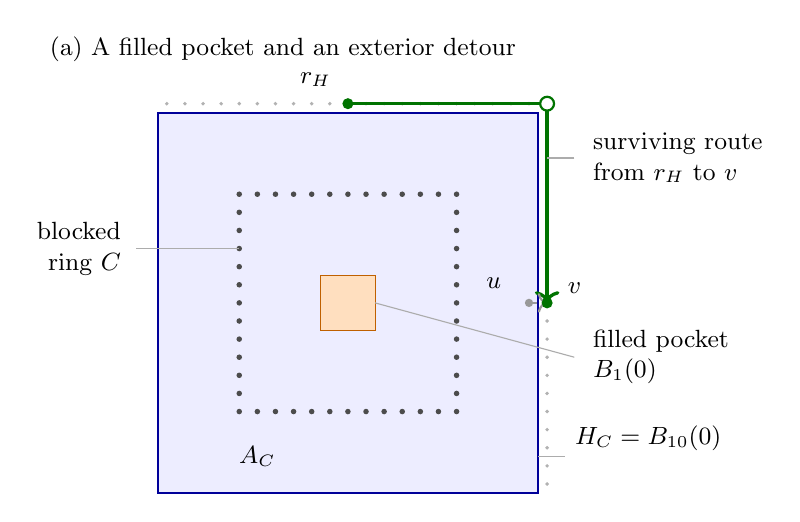
\begin{tikzpicture}[x=.23cm,y=.23cm,font=\small]
  \node[anchor=west] at (-17,14)
    {(a) A filled pocket and an exterior detour};
  \fill[blue!7] (-10.5,-10.5) rectangle (10.5,10.5);
  \draw[blue!60!black,thick] (-10.5,-10.5) rectangle (10.5,10.5);
  \fill[orange!25] (-1.5,-1.5) rectangle (1.5,1.5);
  \draw[orange!75!black] (-1.5,-1.5) rectangle (1.5,1.5);
  \foreach \n in {-6,...,6} {
    \fill[black!70] (\n,6) circle (1pt);
    \fill[black!70] (\n,-6) circle (1pt);
  }
  \foreach \n in {-5,...,5} {
    \fill[black!70] (6,\n) circle (1pt);
    \fill[black!70] (-6,\n) circle (1pt);
  }
  \foreach \n in {-10,...,10} {
    \fill[gray!60] (\n,11) circle (.7pt);
    \fill[gray!60] (11,\n) circle (.7pt);
  }
  \draw[->,green!45!black,very thick] (0,11)--(11,11)--(11,0);
  \draw[->,gray!80,dashed,thick] (10,0)--(11,0);
  \fill[green!45!black] (0,11) circle (2pt);
  \fill[green!45!black] (11,0) circle (2pt);
  \fill[gray!80] (10,0) circle (1.5pt);
  \filldraw[fill=white,draw=green!45!black,thick] (11,11) circle (2.5pt);
  \node[anchor=south east] at (-.4,11.4) {$r_H$};
  \node[anchor=east] at (9,1.1) {$u$};
  \node[anchor=west] at (11.6,.8) {$v$};
  \node at (-5,-8.5) {$A_C$};
  \node[anchor=west] at (12,-7.5) {$H_C=B_{10}(0)$};
  \draw[gray!65] (12,-8.5)--(10.5,-8.5);
  \node[anchor=east,align=right] at (-12,3)
    {blocked\\ring $C$};
  \draw[gray!65] (-11.7,3)--(-6,3);
  \node[anchor=west,align=left] at (13,-3)
    {filled pocket\\$B_1(0)$};
  \draw[gray!65] (12.5,-3)--(1.5,0);
  \node[anchor=west,align=left] at (13,8)
    {surviving route\\from $r_H$ to $v$};
  \draw[gray!65] (12.5,8)--(11,8);
\end{tikzpicture}
\par\medskip
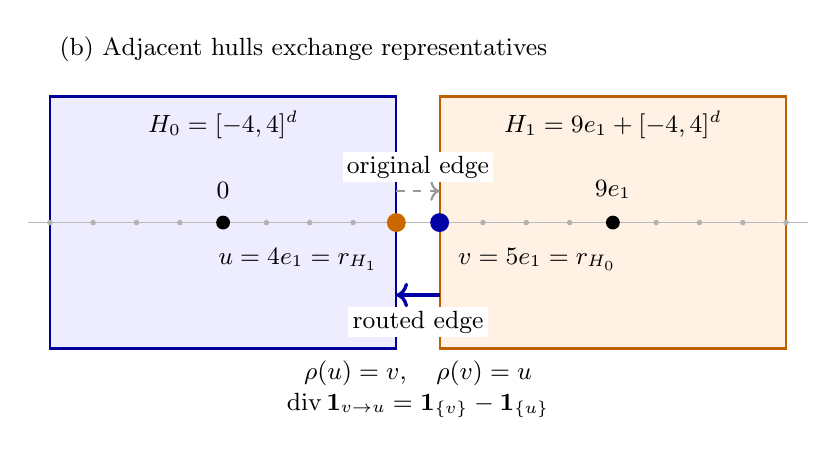
\begin{tikzpicture}[x=.55cm,y=.4cm,font=\small]
  \node[anchor=west] at (-4,5.5)
    {(b) Adjacent hulls exchange representatives};
  \fill[blue!7] (-4,-4) rectangle (4,4);
  \draw[blue!60!black,thick] (-4,-4) rectangle (4,4);
  \fill[orange!10] (5,-4) rectangle (13,4);
  \draw[orange!75!black,thick] (5,-4) rectangle (13,4);
  \draw[gray!55] (-4.5,0)--(13.5,0);
  \foreach \x in {-4,...,13} {\fill[gray!60] (\x,0) circle (1pt);}
  \fill (0,0) circle (2.5pt);
  \fill (9,0) circle (2.5pt);
  \node[above=5pt] at (0,0) {$0$};
  \node[above=5pt] at (9,0) {$9e_1$};
  \node at (0,3.1) {$H_0=[-4,4]^d$};
  \node at (9,3.1) {$H_1=9e_1+[-4,4]^d$};
  \draw[fill=white,blue!65!black,thick] (5,0) circle (3pt);
  \draw[fill=white,orange!80!black,thick] (4,0) circle (3pt);
  \node[anchor=north east] at (3.8,-.5) {$u=4e_1=r_{H_1}$};
  \node[anchor=north west] at (5.2,-.5) {$v=5e_1=r_{H_0}$};
  \draw[->,gray!80,dashed,thick] (4,1)--(5,1);
  \node[above=3pt,fill=white,inner sep=1.5pt] at (4.5,1) {original edge};
  \draw[->,blue!65!black,very thick] (5,-2.3)--(4,-2.3);
  \node[below=4pt,fill=white,inner sep=1.5pt] at (4.5,-2.3) {routed edge};
  \node[align=center] at (4.5,-5.3)
    {$\rho(u)=v,\quad\rho(v)=u$
     \\ $\operatorname{div}\1_{v\to u}=\1_{\{v\}}-\1_{\{u\}}$};
\end{tikzpicture}
\caption{Replacing lattice edges by surviving paths.
In (a), a two-dimensional example, $C=\{z:|z|_\infty=6\}$ is a blocked
ring.  Its radius-four thickening is
$A_C=\{z:2\le|z|_\infty\le10\}$; filling the surviving pocket
$B_1(0)$ gives $H_C=B_{10}(0)$.  The original edge $u\to v$, with
$u=(10,0)$ and $v=(11,0)$, is replaced by the indicated path from
$r_H=(0,11)$ to $v$.  The open corner is a surviving interpolation
vertex outside $S_C$: a nearest-neighbor route need not remain in $S_C$
itself.  In (b), the only blocked sites are $0$ and $9e_1$.
Their filled radius-four hulls are the two
displayed lattice cubes, shown schematically in a coordinate slice; the
transverse scale is compressed.  Both $u=4e_1$ and $v=5e_1$ survive.
Choosing $r_{H_0}=v$ and $r_{H_1}=u$ sends the oriented original edge
$u\to v$ to the reverse edge $v\to u$.  This is the case of
\eqref{eq:adjacent-hull-route} in which the two boundary portions are
empty.  Applying $\rho$ again would undo this required image exchange.
Panel (a) illustrates the definitions in $d=2$; the hull and boundary
properties in every $d\ge2$ are proved in Lemma~\ref{lem:hulls}.}
\label{fig:hull-routing}
\end{figure}

\FloatBarrier

\subsection{A decaying unit flow from every nearby slot}

The topology gives routes for all lattice edges.  Regularity now bounds
their displacement, which will bound the number of routes using any one
target edge.

\begin{proposition}[Decay of a routed unit flow]\label{prop:flow-decay}
Let $d\ge3$, $\nu=1/(100d)$, and suppose the anchor $x$ is regular in the
sense of Definition~\ref{def:regular-anchor}.  Fix the local constant
$M_*$ as in~\eqref{eq:local-radius-choice} and take $R$ sufficiently
large in terms of those fixed constants.  For every available slot $a$
at any site $y\in B_R(x)$ there is a flow $J_a$ on the available-slot
graph such that
\begin{equation}\label{eq:flow-envelope}
 \operatorname{div}J_a=\1_{\{a\}},\qquad
 |J_a(e)|\le C(1+\dist(e,y))^{-k},
 \qquad k=d-1-d\nu.
\end{equation}
In particular, $\sum_e J_a(e)^2<\infty$.
\end{proposition}

\begin{proof}
First we quantify the hull sizes.  A blocked component meeting $B_{10R}(x)$
has fewer than $2d$ vertices.  Otherwise, starting at a vertex there,
a connected exploration would find $2d$ vertices within $2d-1$ component
steps, all in a ball of radius $8(2d-1)\le M_*$, contradicting regularity.
Such a component has diameter at most $8(2d-2)$, and its hull has diameter
at most
\[
 D_{\mathrm{loc}}=8(2d-2)+8.
\]
For a component avoiding $B_{10R}(x)$, let
$b_C=\min_{z\in C}|z-x|_\infty>10R$.  Applying remote regularity at a
minimizer gives
\begin{equation}\label{eq:remote-hull-size}
 \operatorname{diam}H_C\le 2(1+b_C)^\nu+8.
\end{equation}
This also bounds the diameter of its coordinate bounding box.  Since
$\nu<1$, increasing a fixed lower threshold for $R$ makes the right side,
plus any of the fixed enlargements used above, at most $b_C/10$.
All sites of these enlarged boxes then have distance comparable to $b_C$
from every $y\in B_R(x)$.  In particular, no such remote box contains $y$.

Apply the routes following~\eqref{eq:once-only-map}, using fixed choices
of representatives and paths.  The preceding size bounds show that the
route of a lattice edge $e$ lies within distance
\begin{equation}\label{eq:routing-displacement}
 C(1+\dist(e,y))^\nu
\end{equation}
of that edge.  For a local hull this is the fixed bound $D_{\mathrm{loc}}+2$.
For each remote hull incident to $e$, an endpoint of $e$ belongs to its
bounding box, so its $b_C$ is comparable to $1+\dist(e,y)$; now use
\eqref{eq:remote-hull-size}.  The same reasoning applies when the edge
joins two hulls.  These comparisons are uniform over all injection sites
$y\in B_R(x)$.

Choose one canonical available slot $c(z)$ at each unblocked site $z$.
Lift every routed site path to these canonical slots.  All its edges exist
because every pair of available slots across a lattice edge is present.
The map of the original lattice vertices into slots is
$\psi(z)=c(\rho(z))$.  Its preimages are finite: outside the finitely many
finite hulls it is injective, and only those hulls can supply additional
preimages.

We also need a bounded path from the specified slot $a$ to $\psi(y)$.
If $y$ is in a hull, that hull is local and the separation between $y$
and $\rho(y)$ is at most $D_{\mathrm{loc}}+1$.  Both sites are unblocked, so
Lemma~\ref{lem:local-connectivity} joins them through survivors in a
fixed neighborhood of $y$.  Its assumptions hold because $y\in B_R(x)$,
the neighborhood has fixed radius, and $R$ dominates that radius.
Lift this path, starting at $a$.  If $\rho(y)=y$ but $a\ne c(y)$,
use a two-edge path through a surviving neighbor of $y$.  Such a neighbor
exists, since blocking all $2d$ neighbors would violate local regularity.
Thus in all cases there is a simple slot path $Q_a$ from $a$ to $\psi(y)$
of bounded length and displacement.  The choice
$K_{\rm conn}\ge8(2d-2)+12$ in the local-connectivity construction covers
these requirements before $M_*$, $R$, and finally $p$ are fixed.

Start with an explicit unit flow $F_y$ on the full lattice.  In the
positive orthant based at $y$, give each site $y+n$, $n\in\Z_{\ge0}^d$,
$|n|_1=N$, mass
\[
 a_N=\binom{N+d-1}{d-1}^{-1},
\]
and send the fraction $(n_j+1)/(N+d)$ along its edge in direction $e_j$.
Put zero on all other edges.  At a site $y+n$ of level $N\ge1$, the
incoming mass is
\[
 a_{N-1}\frac{\sum_j n_j}{N+d-1}
 =a_{N-1}\frac{N}{N+d-1}=a_N,
\]
which equals its outgoing mass.  The outgoing mass at $y$ is one.
Consequently
\begin{equation}\label{eq:orthant-flow}
 \operatorname{div}F_y=\1_{\{y\}},\qquad
 |F_y(e)|\le C(1+\dist(e,y))^{1-d}.
\end{equation}

For each lattice edge, send its signed $F_y$-value along its lifted simple
path.  To justify this infinite sum and estimate it, fix a target slot
edge $f$ and write $h=\dist(f,y)$.  If the route of an original edge $e$
uses $f$, put $t=\dist(e,y)$.  The displacement bound gives
\[
 |h-t|\le C(1+t)^\nu+C.
\]
Because $\nu<1$, this implies $1+t\asymp1+h$, with uniform constants:
above a fixed threshold the error is at most $(1+t)/2$, and below that
threshold all quantities are bounded.  It follows also that $e$ lies
within distance $C(1+h)^\nu$ of $f$.  There are at most
\begin{equation}\label{eq:target-congestion}
 C(1+h)^{d\nu}
\end{equation}
such lattice edges.  Each routed path is simple, so any one of them uses
$f$ at most once.  Summing~\eqref{eq:orthant-flow} over this finite set
gives a well-defined flow $J_a^0$ with
\[
 |J_a^0(f)|\le C(1+h)^{1-d+d\nu}.
\]
The count~\eqref{eq:target-congestion} already counts all contributions
to $f$; no path-length factor is present.

Local finiteness of the path sum and finiteness of the vertex preimages
justify the divergence calculation at any slot $b$:
\begin{align*}
 \operatorname{div}J_a^0(b)
 &=\sum_{e=(u,v)}F_y(e)
       \bigl(\1_{\{\psi(u)=b\}}-\1_{\{\psi(v)=b\}}\bigr)\\
 &=\sum_{z:\psi(z)=b}\operatorname{div}F_y(z)
 =\1_{\{\psi(y)=b\}}.
\end{align*}
Here one fixed orientation is used for each original lattice edge; the
signed route is always from $\psi(u)$ to $\psi(v)$.  Adding the unit path
flow from $a$ to $\psi(y)$ therefore gives
\[
 J_a=J_a^0+\1_{Q_a},\qquad
 \operatorname{div}J_a=\1_{\{a\}}.
\]
The connector has fixed bounded support near $y$, so enlarging $C$
preserves the envelope~\eqref{eq:flow-envelope}.  Finally,
$2k>d$ for $d\ge3$, and the number of slot edges at radius $h$ is at
most $C(1+h)^{d-1}$.  Squaring the envelope and summing proves finite
energy.  Equivalently, this is a unit flow to infinity: its net outward
flux across any finite vertex set containing $a$ is one.
\end{proof}

\subsection{Overlap and arbitrary subunit injections}

We now combine the individual flows.  Their decay, rather than a
disjointness property of their routes, controls their total energy.

\begin{lemma}[Overlap of two flows]\label{lem:flow-overlap}
Suppose two flows on an available-slot graph obey
\[
 |J(e)|\le C_0(1+\dist(e,y))^{-k},\qquad
 |J'(e)|\le C_0(1+\dist(e,y'))^{-k},
\]
where $d/2<k<d$.  Then
\begin{equation}\label{eq:flow-overlap}
 \sum_e |J(e)J'(e)|
 \le C(1+|y-y'|_\infty)^{-(2k-d)},
\end{equation}
where $C$ depends only on $d,\ell,k,C_0$.
\end{lemma}

\begin{proof}
Write $H=1+|y-y'|_\infty$.  For bounded $H$ the assertion follows by
summing the squared envelopes and Cauchy--Schwarz.  Otherwise, in the
ball of radius $(H-1)/3$ about either center, the other envelope is at
most $CH^{-k}$, whereas the sum of the nearer envelope is at most
$CH^{d-k}$.  These two regions cost $CH^{d-2k}$.  In the remaining
region the two distances are comparable.  Dyadic annuli of radii
comparable to $2^jH$, $j\ge0$, cost at most
\[
 C\sum_{j\ge0}(2^jH)^{d-2k}\le CH^{d-2k},
\]
since $2k>d$.  Changing a site distance to the distance from an incident
edge changes it by at most one, and the number of slot edges per site
is bounded by $2d\ell^2$.  Thus the same estimates apply to the stated
edge sum.
\end{proof}

\begin{proposition}[Energy for arbitrary injections]\label{prop:flow-energy}
Let $d\ge3$, $\alpha=1/100$, and $\nu=1/(100d)$.  Fix $M_*$ as in
\eqref{eq:local-radius-choice} and take $R$ sufficiently large as in
Proposition~\ref{prop:flow-decay}.  Let $T$ be a finite
set of $m$ anchor slots with sites $x_i$, satisfying
\[
 \#\{i\in T:x_i\in B_h(z)\}\le L(1+h)^\alpha
 \quad\text{for all }z\in\Z^d,\ h\ge0.
\]
Fix an available-slot graph and a subset $I\subset T$ of anchors regular
for this graph.  For each $i\in I$, let $\mu_i$ be any nonnegative mass
on its slots, supported over $B_R(x_i)$ and satisfying
$\sum_a\mu_i(a)\le1$.  There is a flow $J$ such that
\begin{equation}\label{eq:injection-flow-energy}
 \operatorname{div}J=\sum_{i\in I}\mu_i,
 \qquad \sum_e J(e)^2\le C|I|R^\alpha\le CmR^\alpha.
\end{equation}
Consequently every finitely supported real function $g$ on the graph
satisfies
\begin{equation}\label{eq:injection-pairing}
 \left|\left\langle\sum_{i\in I}\mu_i,g\right\rangle\right|
 \le \bigl(CmR^\alpha\mathcal D(g)\bigr)^{1/2},
 \qquad \mathcal D(g)=\frac12\sum_e(g(e^-)-g(e^+))^2.
\end{equation}
All constants are uniform over the choices of $I$ and of the masses.
\end{proposition}

\begin{proof}
The empty case uses $J=0$.  Otherwise, for each slot $a$ in the support
of $\mu_i$, take a unit flow $J_{i,a}$ from
Proposition~\ref{prop:flow-decay}, using anchor $x_i$, and set
\[
 J=\sum_{i\in I}\sum_a\mu_i(a)J_{i,a}.
\]
This is a finite linear combination, and its divergence is as asserted.
Put $q=2k-d=d-2-2d\nu>\alpha$.  By
Lemma~\ref{lem:flow-overlap}, the absolute overlap of $J_{i,a}$ and
$J_{j,b}$ is at most $C(1+|y_a-y_b|_\infty)^{-q}$, where $y_a,y_b$
are the sites of their injection slots.  If $|x_i-x_j|_\infty>4R$,
then $|y_a-y_b|_\infty\ge |x_i-x_j|_\infty/2$, uniformly over both
supports.  For the remaining anchor pairs use the uniform constant
overlap bound.  The mass bound of one per anchor therefore gives
\[
 \sum_eJ(e)^2\le C\sum_{i\in I}
 \left[\#\{j\in I:|x_j-x_i|_\infty\le4R\}
 +\sum_{\substack{j\in I\\|x_j-x_i|_\infty>4R}}
     (1+|x_j-x_i|_\infty)^{-q}\right].
\]
The first term is at most $CL R^\alpha$.  Splitting the second into
annuli $2^j4R<|x_j-x_i|_\infty\le2^{j+1}4R$ bounds it by
\[
 CL\sum_{j\ge0}(2^jR)^{\alpha-q}\le C,
\]
because $R\ge1$ and $q>\alpha$.  This proves
\eqref{eq:injection-flow-energy}, including repeated anchor sites since
the growth assumption counts slots.

Finally, finite support of $g$ permits summation by divergence without a
term at infinity:
\[
 \left\langle\sum_i\mu_i,g\right\rangle
 =\sum_e J(e)(g(e^-)-g(e^+)).
\]
Cauchy--Schwarz and $\sum_e|\nabla_e g|^2=2\mathcal D(g)$ give
\eqref{eq:injection-pairing}.  In particular it applies to functions that
vanish on the killed boundary and outside the physical box, with exactly
the energy normalization in~\eqref{eq:slot-energy}.
\end{proof}

The construction is deterministic at a single slice.  Thus the masses
and the set of regular anchors may depend on the whole exposed
environment; the pairing bound requires neither independence nor a
choice of flows continuous in time.

\section{Heat-flow leakage and the pin bootstrap}\label{sec:leakage}

We now use the geometric estimates to bound the return fraction in the
simultaneous pin test.  The main task is to prove that the hitting
function loses nearly $m$ units of squared norm during each of two short
portions of a period, where $m$ is the number of new pins.  Local diffusion
spreads the mass on those pins, and the flow estimate controls its pairing
with the rest of the hitting function.  Averaging the accumulated heat
dissipation will absorb this pairing.
The Nash method for Markov semigroups is developed in
\cite[Section~3]{DiaconisSaloffCoste1996}.  The proof below accounts
explicitly for the changing hole sets, killing, instantaneous
contractions, and the restriction of the Nash inequality to regular
times.

Throughout the section, $d\ge3$, $\ell=2S$, and $\Lambda$ is a finite cube.
We use the parameters of Section~\ref{sec:sparse}, namely
\[
 \alpha=\frac1{100},\qquad \nu=\frac1{100d},\qquad
 a=\frac{11}{10},\qquad s=p^{-a},\qquad R=\lceil C_*s\rceil,
 \qquad \beta\ge5s.
\]
The spatial growth constant $L$, the regularity radius $M_*$, and the
constant $C_*$ will be fixed independently of the final choice of $p$.
The test $T$ consists of $m\ge1$ distinct slot points at one time, is
disjoint from $E\supseteq D_0$, and satisfies
\begin{equation}\label{eq:leakage-growth}
 \#\{i\in T:x_i\in B_h(z)\}\le L(1+h)^\alpha
 \quad(z\in\Z^d,\ h\ge0).
\end{equation}
Here $x_i$ denotes the site of the slot point $i$.
Write $P=E\cup T$, and sample the exposed paths under $\mathbb P_P$,
as in Proposition~\ref{prop:exposure}.  Expectations of quantities
determined by these paths use their actual marginal, including the factor $g_P$ in
\eqref{eq:exposure-outer-law}.  At a fixed exposure, the propagators use
the unconditioned fresh-turn walk.  As in
Proposition~\ref{prop:pin-test}, $r$ is the
expected fraction of points of $T$ whose next pin along the actual
cycle again belongs to $T$.

Recall the one-period, column-forward kernel $U$ of the fresh-turn walk,
killed on visiting $D_0$.  At the cut containing $T$, the function $f$
of Lemma~\ref{lem:return-energy} is $1$ on $T$ and, off $T$, is the
probability of a future visit to $T$ before killing, namely the minimal
nonnegative hitting solution.
In particular,
\begin{equation}\label{eq:leakage-hitting-input}
 0\le f\le1,\qquad f|_{\partial\Lambda}=0,\qquad
 U^*f=f\ \hbox{off }T,\qquad
 m(1-r)\ge\mathbb E_P\langle f,(I-U)f\rangle.
\end{equation}
The last inequality incorporates the conditional first-moment identity
of Proposition~\ref{prop:first-moment} and the relaxation of the other
pins of $E$.  A class of the relaxed walk that never reaches $T$ has
$f=0$; certain absorption is unnecessary.  In particular $f$ is a
function of the exposed paths, and we will not require it to be
independent of any geometric event.
All the propagators below are measurable functions of finite-jump
data.  The hitting function is measurable as the increasing limit of
finite-horizon hitting probabilities, so the expectations used below
are well defined.

For grid pin sets satisfying the larger-pin induction hypothesis
$\mathsf I_p(P)$ of \eqref{eq:induction-assertion}, our aim is
\begin{equation}\label{eq:leakage-target}
 \mathbb E_P\langle f,(I-U)f\rangle\ge m[1-\varepsilon(p)],
 \qquad \varepsilon(p)=o(p).
\end{equation}
Together with \eqref{eq:leakage-hitting-input}, this gives
$r\le\varepsilon(p)$.  The simultaneous pin test then recovers
$\mathbb P_E(T\subseteq\mathcal B_E)\le p^m$ once
$2\varepsilon(p)\le p$, closing the induction step.
To obtain \eqref{eq:leakage-target}, split
$f=\eta+g$, where $\eta=\1_T$ and $g=f-\eta$.
Then $0\le g\le1$ and $\langle\eta,g\rangle=0$.
We first relate the quadratic form to norm losses at both ends of the
period.  The Nash estimate will make the propagated $\eta$ small in
squared norm, while the flow estimate will control its pairing with the
propagated $g$ through the square root of that function's energy at the
same time.

\subsection{Ordered propagation and the two ends of a period}

We first fix one exposed environment.  Between its finitely many
instantaneous changes, the surviving interior holes carry the symmetric
rate-$1/2$ heat equation.  A boundary hole is assigned value zero.  Thus
the generator on an interior hole $k$ is
\begin{equation}\label{eq:leakage-generator}
 (L_t v)_k=\frac12\sum_{j:\{j,k\}\text{ is an available slot edge}}
                   (\widetilde v_j-v_k),
\end{equation}
where $\widetilde v$ equals $v$ on interior holes and zero on boundary
holes.  The diagonal includes the escape rates to the boundary.  This
is continuous killing throughout the heat interval.

At an instantaneous change, let $F$ be the forced bijection or the
average of the allowed within-site completion bijections, from the
hole set just before the change to that just after it.  If $R_-$ and
$R_+$ are the projections deleting killed coordinates on those two
sets, respectively, the killed factor is
\begin{equation}\label{eq:ordered-killing}
             R_+FR_-,\qquad
             (R_+FR_-)^*=R_-F^*R_+.
\end{equation}
The projections remain in this order.  For heat intervals, the
corresponding assertion follows either from the symmetric Dirichlet
generator or by transposing the sampled surviving paths.

By the subpermutation argument in \eqref{eq:hole-contractions}, these
matrices, their products, and their adjoints are nonnegative, have row
and column sums at most one, and contract the counting $\ell^2$ norm.
We will also use the two sum bounds separately: the row bound gives
$0\le Av\le1$ when $0\le v\le1$, while the column bound gives
$\|Av\|_1\le\|v\|_1$ for $v\ge0$.

Put the time of $T$ at the beginning and end of a period.  Let $C_u$ be
the initial propagation of duration $u$, and let $C_u^{\rm rev}$ be
the adjoint of the ending propagation of duration $u$.
Forward propagation includes the changes after its initial cut through
its final cut, under the post-completion convention at time zero.
Reverse propagation traverses precisely those factors in the opposite
order.  If the ending cut is a completion cut, its adjoint completion
is the first factor traversed in reverse time.  It is included exactly
once, including when it occurs immediately at elapsed time zero.
We set $C_0=C_0^{\rm rev}=I$ on the initial, already unkilled
coordinates and count any such initial reverse jump in every positive
duration that traverses it.  This convention allows a contraction jump
at $u=0+$.

\begin{lemma}[Leakage at both ends]\label{lem:two-ends}
For every fixed exposed environment, $s>0$, and period $\beta\ge4s$,
the preceding killed propagators satisfy, for every real vector $v$
on the holes at the distinguished cut with zero boundary values,
\begin{equation}\label{eq:two-ends}
 \langle v,(I-U)v\rangle\ge\frac12\left(
   \|v\|_2^2-\|C_{2s}v\|_2^2
  +\|v\|_2^2-\|C_{2s}^{\rm rev}v\|_2^2\right).
\end{equation}
Both $u\mapsto\|C_uv\|_2$ and
$u\mapsto\|C_u^{\rm rev}v\|_2$ are nonincreasing.
\end{lemma}

\begin{proof}
The nonoverlapping initial and ending portions factor $U=BMA$, with
$A=C_{2s}$, $B^*=C_{2s}^{\rm rev}$, and $M$ the intervening
propagation.  At $\beta=4s$, assign every shared-cut jump once according
to the preceding convention and take the intervening identity on that
cut.  All factors are contractions, so
\[
 \langle v,Uv\rangle
 =\langle B^*v,MAv\rangle
 \le\|B^*v\|_2\|Av\|_2
 \le\tfrac12\bigl(\|B^*v\|_2^2+\|Av\|_2^2\bigr).
\]
This proves \eqref{eq:two-ends}.  Longer initial portions are obtained
by left multiplication by further contraction factors.  For the ending
adjoints the same fact follows after reversing the factor order, using
\eqref{eq:ordered-killing}.  It proves both monotonicity assertions.
\end{proof}

The reverse construction has symmetric heat between changes, inverse
forced transports, averages of inverse completion bijections, and the
ordered killing projections.  Thus it has the same deterministic
analytic properties as forward propagation.  Its environment is the
original exposed environment read in reverse order; no invariance of
the environment law under time reversal is asserted or needed.

Thus \eqref{eq:leakage-target} will follow if each of these two
propagations loses at least $m[1-\varepsilon(p)]$ in expected squared
norm by time $2s$.  We prove both estimates through the same argument.

For the rest of the estimates, $C_u$ denotes either of the two
propagations, and $t(u)$ denotes its physical time slice modulo $\beta$.
On the available slot graph, extended by all slots outside $\Lambda$,
use the energy
\[
 \mathcal D_{t}(v)=\frac12\sum_{\{j,k\}\text{ available at }t}
                          (v_j-v_k)^2.
\]
Vectors propagated in the box are extended by zero on its boundary and
outside.  Since the boundary is the inner boundary, any edge crossing
out of the box has two zero values.

Write $\eta_u=C_u\eta$,
$g_u=C_ug$, and
$\mathcal L(u)=\|f\|_2^2-\|C_uf\|_2^2$.
For a jump traversed at elapsed time $v$, let
\[
 \Delta_g(v)=\|g_{v,\mathrm{before}}\|_2^2
                  -\|g_{v,\mathrm{after}}\|_2^2\ge0.
\]
Here ``before'' and ``after'' refer to the chosen direction of
propagation.  Denote the finite list of jumps traversed by duration
$u$ by $\mathcal J(u)$, including an initial reverse jump when present.
Between jumps, \eqref{eq:leakage-generator} gives
\[
 \frac{\mathrm d}{\mathrm du}\|g_u\|_2^2
     =-2\mathcal D_{t(u)}(g_u).
\]
To check the normalization, an interior--interior edge contributes
$-(g_j-g_k)^2$ to this derivative, and an interior--boundary edge
contributes $-g_j^2$.  These are exactly the contributions to
$-2\mathcal D$.  Summing continuous and instantaneous losses and then
expanding $\|\eta_u+g_u\|_2^2$ yields the exact identity
\begin{align}
 \mathcal L(u)
 &=m-\|\eta_u\|_2^2-2\langle\eta_u,g_u\rangle\notag\\
 &\quad+2\int_0^u\mathcal D_{t(v)}(g_v)\,\mathrm dv
       +\sum_{v\in\mathcal J(u)}\Delta_g(v).
       \label{eq:exact-loss}
\end{align}
The sum includes a completion at an endpoint whenever that completion
is a factor of the propagation.  Dropping it gives
\begin{equation}\label{eq:loss-lower}
 \mathcal L(u)\ge
 m-\|\eta_u\|_2^2-2\langle\eta_u,g_u\rangle
       +2\int_0^u\mathcal D_{t(v)}(g_v)\,\mathrm dv.
\end{equation}
Keeping this as an inequality is necessary even when a completion is
the only nontrivial instantaneous operation.

\subsection{Localization with actual and fresh marks}

For $i\in T$, let $\eta_{i,u}$ be the propagation from unit mass at $i$,
with the additional rule that a path is killed when its site leaves
$B_R(x_i)$.  Use this additional killing for continuous moves and on
both sides of instantaneous changes.  Positivity and the path
description give
\begin{equation}\label{eq:local-pieces}
 0\le\zeta_u:=\sum_{i\in T}\eta_{i,u}\le\eta_u\le1,
 \qquad \|\eta_{i,u}\|_1\le1.
\end{equation}

\begin{lemma}[Localization averaged over the pin law]\label{lem:localization}
Fix $d$ and $\ell$.  There is a constant $C_*=C_*(d,\ell)$ such that
for $s\ge1$, $R=\lceil C_*s\rceil$, $\beta\ge5s$, every finite
cube, every $E\supseteq D_0$ consisting of $D_0$ and finitely many
pins, and every disjoint single-time test $T$, one has
\begin{equation}\label{eq:localization}
 \mathbb E_P\|\eta_u-\zeta_u\|_1\le C m e^{-cs}
       \qquad(0\le u\le2s)
\end{equation}
for either direction of propagation.  The constants are independent of
the volume, the pin sets, $\beta$, and $s$.
\end{lemma}

\begin{proof}
First sample a complete actual exchange picture with law
$\mathbb P_P$ and expose its missing cycles.  Conditional on that
exposure, realize the unconditioned one-particle propagation of
Proposition~\ref{prop:exposure} using independent fresh rate-$1/2$
Poisson clocks on all slot edges, accepting a fresh mark only when its
two endpoints are holes.  The forced moves use marks of the actual
picture.  Completion randomness changes slots only within a site.
This construction is for the unconditioned fresh walk; its exposure
still has the marginal induced by the full pin law.

The difference in \eqref{eq:local-pieces}, summed over output slots, is
bounded by the sum of the probabilities that these individual walks
exit their respective balls before elapsed time $u$.  Exiting requires
at least $R$ nearest-neighbor spatial steps.  The first $R$ such steps
give a chronological list of marks, each from either the actual
picture or the fresh family.  For a fixed list of sites, slot edges,
and choices of source, the actual marks used are distinct: the time
interval has length at most $2s<\beta$, so its image on the time circle
does not use a mark twice.  This remains true if the interval crosses
time zero, and if it is traversed backwards.  Fresh marks in the list
are distinct as well.

Suppose a source choice uses $k$ actual marks and $R-k$ fresh marks.
By Lemma~\ref{lem:factorial}, the joint factorial measure of the
actual marks is bounded by $2^k$ times their base product intensity.
Independence of the fresh family then bounds the mixed measure by
\[
        1^k(1/2)^{R-k}\,\mathrm dt_1\cdots\mathrm dt_R
\]
on the prescribed edge coordinates.  All source choices are integrated
over the same ordered simplex
$0<t_1<\cdots<t_R<u$, of volume $u^R/R!$.
At each spatial step there are at most $2d\ell^2$ choices for the next
site and the slot edge, even if one ignores constraints from the
current slot.  Summing source choices and edge choices therefore bounds
the expected number of such lists, for one initial point, by
\begin{equation}\label{eq:mixed-factorial-count}
 (2d\ell^2)^R(1+1/2)^R\frac{u^R}{R!}
       \le\frac{(2Ks)^R}{R!},\qquad K=3d\ell^2.
\end{equation}
The existence of an exit path is bounded by this count; the counted
lists need not themselves be realizable walk histories.  In
particular, the restrictions imposed by the exposure can be ignored
when taking this upper bound.  No factorial bound conditional on a
fixed exposure has been used.

Since $R!\ge(R/e)^R$, choosing $C_*>4eK$ bounds the last expression
by $2^{-R}\le e^{-cs}$.  Sum over $i\in T$ to obtain
\eqref{eq:localization}.  Transposition merely reverses the
chronological lists and the forced transports.  The same mixed
factorial estimate applies under the original law $\mathbb P_P$,
which proves the reverse assertion too.
\end{proof}

\subsection{Diffusion during regular times}

We now use the downward-induction hypothesis only through the three
proved inputs from Sections~\ref{sec:sparse} and~\ref{sec:flows}.
Assume $\mathsf I_p(P)$, as defined in
\eqref{eq:induction-assertion}.  With the fixed choices of constants
there, Proposition~\ref{prop:regularity} gives
\begin{equation}\label{eq:leakage-delta}
 \mathbb P_P(t\text{ is not regular for }i)
       \le\delta:=C R^d p^{2d}+C e^{-cR^\xi}
       \quad(i\in T, t\in[0,\beta)),
\end{equation}
where $\xi>0$ and the constants are fixed for all $p$ below a
preliminary threshold.  At a regular slice,
Proposition~\ref{prop:local-nash} states
\begin{equation}\label{eq:leakage-nash-input}
 \|v\|_2^{2+4/d}\le C\mathcal D_t(v)\|v\|_1^{4/d}
\end{equation}
for nonnegative $v$ supported on surviving slots above $B_R(x_i)$,
with zero extension.  Finally, Proposition~\ref{prop:flow-energy}
applies to any subset of the anchors regular at that same time and to
any nonnegative injections of mass at most one per anchor supported
above its $R$-ball.  Their sum is the divergence of a flow $J$ with
\begin{equation}\label{eq:leakage-flow-input}
                   \sum_e J(e)^2\le C mR^\alpha.
\end{equation}
The flow estimate follows from Proposition~\ref{prop:flow-decay} and
the growth condition; its applicability to arbitrary injection points
and subunit masses is part of its statement.

\begin{lemma}[Decay after enough regular time]\label{lem:regular-time-decay}
Let $T$ satisfy \eqref{eq:leakage-growth}, and assume
$\mathsf I_p(P)$ for $P=E\cup T$, with $p$ below the preliminary
threshold in Proposition~\ref{prop:regularity}.  For the localized
propagators defined above, in either direction and for
$s\le u\le2s$,
\begin{align}
 \mathbb E_P\|\eta_{i,u}\|_2^2
       &\le C(s^{-d/2}+\delta)\quad(i\in T),
                    \label{eq:piece-decay}\\
 \mathbb E_P\|\eta_u\|_2^2
       &\le C m\bigl[e^{-cs}+R^\alpha(s^{-d/2}+\delta)\bigr].
                    \label{eq:all-pieces-decay}
\end{align}
\end{lemma}

\begin{proof}
Put $q_i(u)=\|\eta_{i,u}\|_2^2$.  All localized factors are
contractions, so $0\le q_i\le1$ and $q_i$ is nonincreasing,
including at jumps.  Between jumps the additional killing gives the
Dirichlet generator with zero values outside $B_R(x_i)$ as well as
on the physical boundary.  Consequently, at every regular smooth
time, \eqref{eq:leakage-nash-input} and
$\|\eta_{i,u}\|_1\le1$ imply
\begin{equation}\label{eq:nash-differential}
 q_i'(u)=-2\mathcal D_{t(u)}(\eta_{i,u})
                         \le-c q_i(u)^{1+2/d}.
\end{equation}
At other smooth times $q_i'\le0$.
As long as $q_i>0$, the function $q_i^{-2/d}$ thus increases at a
fixed positive rate during regular time and cannot decrease at other
times or jumps.  If $q_i$ reaches zero, it stays zero.  It follows in
either case that
\[
 \int_0^s\1_{\{t(v)\text{ regular for }i\}}\,\mathrm dv\ge s/2
 \quad\Longrightarrow\quad
 q_i(u)\le C s^{-d/2}\quad(s\le u\le2s).
\]
The expected amount of nonregular time in $[0,s]$ is at most
$s\delta$ by \eqref{eq:leakage-delta} and Fubini.  Markov's
inequality bounds the probability of its exceeding $s/2$ by
$2\delta$.  This proves \eqref{eq:piece-decay}.  For reverse
propagation, $t(v)$ simply runs in the opposite direction; the same
fixed-time estimate \eqref{eq:leakage-delta} gives the same integral
bound, without changing the probability law.

At any slot above $z$, only anchors with $x_i\in B_R(z)$ can
contribute to $\zeta_u$.  Their number is at most
$L(1+R)^\alpha\le C R^\alpha$ by
\eqref{eq:leakage-growth}.  Hence pointwise Cauchy--Schwarz and
summation give
\[
                \|\zeta_u\|_2^2\le C R^\alpha\sum_{i\in T}q_i(u).
\]
Since $0\le\zeta_u\le\eta_u\le1$,
\[
 \|\eta_u\|_2^2-\|\zeta_u\|_2^2
       =\sum_k(\eta_u(k)-\zeta_u(k))(\eta_u(k)+\zeta_u(k))
       \le2\|\eta_u-\zeta_u\|_1.
\]
Use Lemma~\ref{lem:localization} and \eqref{eq:piece-decay} to
obtain \eqref{eq:all-pieces-decay}.
\end{proof}

The initial pin mass has now spread sufficiently in mean square.
The remaining term in \eqref{eq:loss-lower} is its pairing with
$g_u$.  We next use flows at the very slice where this pairing occurs,
so that the positive heat energy can absorb it.

\subsection{Absorbing the interaction at the same time}

\begin{proposition}[Expected leakage]\label{prop:leakage}
Fix the constants in the preceding geometric estimates and choose
$C_*$ as in Lemma~\ref{lem:localization}.  For all sufficiently small
$p>0$, every finite cube, every circular grid of mesh at most $p^{4d}$,
every $E$ consisting of $D_0$ and grid pins, and every disjoint
single-time grid test $T$ satisfying \eqref{eq:leakage-growth}, assume
$\mathsf I_p(P)$ for $P=E\cup T$.  If $\beta\ge5s$, then, for
each of the forward and reverse propagations,
\begin{equation}\label{eq:expected-leakage}
 \mathbb E_P\bigl[\|f\|_2^2-\|C_{2s}f\|_2^2\bigr]
             \ge m[1-\varepsilon(p)],
\end{equation}
where one may take
\begin{equation}\label{eq:epsilon-definition}
 \varepsilon(p)=C\left[e^{-cs}
       +R^\alpha\left(s^{-d/2}+\delta+s^{-1}\right)\right],
 \qquad \delta=C R^d p^{2d}+C e^{-cR^\xi}.
\end{equation}
All constants are independent of the volume, period, grid, pin sets,
and final $p$.
\end{proposition}

\begin{proof}
For $s\le u\le2s$, let
\[
 \mu_u=\sum_{i:\,t(u)\text{ regular for }i}\eta_{i,u}.
\]
By \eqref{eq:local-pieces}, $0\le\mu_u\le\eta_u$.
The nonnegative discarded mass is bounded by the localization error
plus the masses attached to nonregular anchors.  Since $0\le g_u\le1$
and each local mass is at most one, Lemma~\ref{lem:localization} and
\eqref{eq:leakage-delta} give
\begin{equation}\label{eq:discarded-pairing}
 \mathbb E_P\langle\eta_u-\mu_u,g_u\rangle
                         \le C m(e^{-cs}+\delta).
\end{equation}
This uses only pointwise bounds, so dependence of $g_u$ on the same
environment causes no change.

At a fixed regular slice, each summand of $\mu_u$ meets exactly the
support and mass hypotheses of \eqref{eq:leakage-flow-input}.  Choose
a reference orientation for the available edges, with
$\operatorname{div}J$ equal to outgoing minus incoming flow.  Since
$g_u$ is finitely supported, summation by parts has finitely many
nonzero terms and gives
\[
 \langle\mu_u,g_u\rangle
   =\sum_{e=(j,k)}J(e)(g_u(j)-g_u(k)).
\]
Cauchy--Schwarz, \eqref{eq:leakage-flow-input}, and
$\sum_e|\nabla_e g_u|^2=2\mathcal D_{t(u)}(g_u)$ imply the
deterministic inequality
\begin{equation}\label{eq:same-time-pairing}
       |\langle\mu_u,g_u\rangle|
          \le\bigl(A\mathcal D_{t(u)}(g_u)\bigr)^{1/2},
               \qquad A=C m R^\alpha.
\end{equation}
It suffices that a flow exists at each time: the resulting inequality
contains only measurable propagated vectors and energies, so no
measurable or continuous choice of flows is required.

To make the remainder in weighted Young's inequality integrable at the
final time, use an averaging density that vanishes linearly there; its
tail weight then vanishes quadratically.
Average \eqref{eq:loss-lower} over $u\in[s,2s]$ with probability
density
\[
 w(u)=\frac{2(2s-u)}{s^2},\qquad
 W(u)=\int_u^{2s}w(v)\,\mathrm dv=\frac{(2s-u)^2}{s^2}.
\]
Since $\mathcal L$ is nondecreasing,
$\mathcal L(2s)\ge\int_s^{2s}w(u)\mathcal L(u)\,\mathrm du$.
Tonelli's theorem shows that the positive energy in this average
contains
\[
                  2\int_s^{2s}W(u)\mathcal D_{t(u)}(g_u)\,\mathrm du;
\]
the additional contribution from $[0,s]$ is nonnegative.
At each $s\le u<2s$, weighted Young's inequality gives
\begin{equation}\label{eq:weighted-young}
 2w(u)\sqrt{A\mathcal D_{t(u)}(g_u)}
 \le2W(u)\mathcal D_{t(u)}(g_u)+\frac{A w(u)^2}{2W(u)}.
\end{equation}
The same-time energy has therefore absorbed the retained pairing.
The remaining integral is finite, because
\begin{equation}\label{eq:weight-integral}
                \int_s^{2s}\frac{w(u)^2}{W(u)}\,\mathrm du=\frac4s.
\end{equation}
The endpoint $u=2s$ has measure zero; the quotient has the constant
value $4/s^2$ on $[s,2s)$.

Taking expectation, using \eqref{eq:discarded-pairing}, and then
Lemma~\ref{lem:regular-time-decay}, we conclude that
\begin{align*}
 \mathbb E_P\mathcal L(2s)
 &\ge m
  -C m\bigl[e^{-cs}+R^\alpha(s^{-d/2}+\delta)\bigr]
  -C m(e^{-cs}+\delta)-C mR^\alpha/s\\
 &\ge m\left[1-C\left(e^{-cs}
                   +R^\alpha(s^{-d/2}+\delta+s^{-1})\right)\right].
\end{align*}
Here $R\ge1$ allows the unweighted $\delta$ error to be included
in $R^\alpha\delta$.  Every step applied to either ordered
propagation, which proves both assertions.
\end{proof}

\subsection{Choosing the constants and closing the finite induction}

The error has enough room to recover the assumed sparsity with the
same parameter $p$.  Indeed, after $C_*$ is fixed, $R$ is comparable
to $s=p^{-a}$ for $p\le1$.  The nonexponential errors $R^\alpha/s$,
$R^\alpha s^{-d/2}$, and $R^{\alpha+d}p^{2d}$ in
\eqref{eq:epsilon-definition} are bounded by constant multiples of
\begin{equation}\label{eq:leakage-exponents}
 p^{a(1-\alpha)},\qquad
 p^{a(d/2-\alpha)},\qquad
 p^{2d-a(d+\alpha)},
\end{equation}
respectively.  Their exponents satisfy
\[
 a(1-\alpha)=\frac{1089}{1000}>1,\qquad
 a(d/2-\alpha)\ge\frac{1639}{1000}>1,\qquad
 2d-a(d+\alpha)\ge\frac{2689}{1000}>1.
\]
The last two lower bounds use $d\ge3$; each exponent increases with
$d$.  Both $e^{-cs}$ and $R^\alpha e^{-cR^\xi}$ are smaller than
every fixed power of $p$.  Thus
\begin{equation}\label{eq:epsilon-small}
                         \varepsilon(p)=o(p)\quad(p\downarrow0).
\end{equation}

For clarity, the constant choices can be made in the following order.
Fix $d,\ell,\alpha,\nu,a$.  Fix the witness scale $b$ and then its
growth constant $L\ge\max\{2d,\ell,4\}$ as in
Lemma~\ref{lem:component-tail}.  Fix the local connectivity radii
and a sufficiently large $M_*$ for
Proposition~\ref{prop:local-nash} and the hull and flow constructions
of Lemma~\ref{lem:hulls} and Proposition~\ref{prop:flow-decay}.
Fix a preliminary $p_0>0$ that absorbs the admissible witness count
in Lemma~\ref{lem:component-tail}; retain the resulting fixed
constants in Proposition~\ref{prop:regularity}, including $c$ and
$\xi$.  Next choose $C_*$ for
Lemma~\ref{lem:localization}.  Finally reduce $p\le p_0$ so that
$R$ exceeds the fixed local radii and the fixed lower bounds needed
for the flow comparisons, $p<1/4$, and
$2\varepsilon(p)\le p$.  The limit
\eqref{eq:epsilon-small} permits all of these final requirements
simultaneously.  No constant in the component tail is recomputed
using this final $p$.

\begin{theorem}[Uniform pin estimate]\label{thm:pin-bootstrap}
For every integer $d\ge3$ and integer slot multiplicity $\ell\ge1$, there
exist $L\ge\max\{2d,\ell,4\}$ and $p_*\in(0,1/4)$ with the
following property.  Let $0<p\le p_*$ and
$\beta\ge5p^{-11/10}$.  In any finite cube $\Lambda$, choose a
finite circular time grid containing zero and of mesh at most
$p^{4d}$.  Let $E$ consist of $D_0$ and any subset of the slot
points on this grid.  Then every nonempty test $T$ at a single grid
time, disjoint from $E$ and satisfying
\eqref{eq:leakage-growth}, obeys
\begin{equation}\label{eq:bootstrap-closed}
                  \mathbb P_E(T\subseteq\mathcal B_E)\le p^{|T|}.
\end{equation}
In particular, with $p=p_*$ and
$\beta_0=5p_*^{-11/10}<\infty$, for every finite
$\beta\ge\beta_0$, every cube, and every slot $j$ at time zero,
\begin{equation}\label{eq:singleton-missing}
                  \mathbb P_{D_0}(j\in\mathcal B_{D_0})\le p_*.
\end{equation}
The constants depend only on $d$ and $\ell$.
\end{theorem}

\begin{proof}
Fix all auxiliary constants in the stated order and choose $p_*$ so
that every $0<p\le p_*$ meets the final requirements.  The set of
interior slot points on a fixed finite grid is finite.  Induct on the
number of these points missing from $E$.  When none is missing there
is no disjoint nonempty test, so $\mathsf I_p(E)$ holds vacuously.

Assume the assertion for pin sets with fewer missing grid points than
$E$, and let $T$ be a test for $E$.  Since $T$ is nonempty and
disjoint from $E$, the set $P=E\cup T$ has strictly fewer missing
points.  The induction hypothesis therefore supplies
$\mathsf I_p(P)$, exactly the hypothesis used in
Proposition~\ref{prop:regularity} and
Proposition~\ref{prop:leakage}.  The two leakage estimates and
Lemma~\ref{lem:two-ends} give
\[
             \mathbb E_P\langle f,(I-U)f\rangle
                         \ge m(1-\varepsilon(p)).
\]
By Lemma~\ref{lem:return-energy}, or
\eqref{eq:leakage-hitting-input}, it follows that
$r\le\varepsilon(p)$.  Proposition~\ref{prop:pin-test} now yields
\[
 \mathbb P_E(T\subseteq\mathcal B_E)
        \le(2r)^m\le(2\varepsilon(p))^m\le p^m.
\]
This proves the induction step for every allowed $T$, and finiteness
of the grid completes the induction.  A singleton interior slot test
at time zero satisfies the growth bound, so taking $E=D_0$ gives
\eqref{eq:singleton-missing}.  A boundary slot belongs to $D_0$,
and its missing-cycle probability is zero.  This covers all slots.
\end{proof}

Theorem~\ref{thm:pin-bootstrap} supplies the uniform missing-cycle
bound required for the magnetization argument.  The grid and the
larger pin sets were devices for a finite induction; the conclusion
\eqref{eq:singleton-missing} concerns the original continuous
boundary pins alone.

\section{From pinned loops to a magnetized equilibrium state}\label{sec:kms}

Theorem~\ref{thm:pin-bootstrap} says that, under boundary pinning,
each slot has small probability of belonging to a cycle that misses the
boundary.  We now turn that statement into a state for the original
zero-field dynamics.  First we obtain a tail bound for the exact spectral
distribution of total magnetization in a free box.  A field tending to
zero selects that tail, and translation averages produce a state with
positive magnetization.  The last step verifies both boundary values of
the KMS strip for that same state.

Fix \(d\geq3\) and \(S\in\{\tfrac12,1,\tfrac32,\ldots\}\).
Let \(p_*\) be the threshold supplied by Theorem~\ref{thm:pin-bootstrap}
for \(\ell=2S\), and put \(p=p_*\) and
\(\beta_0(d,S)=5p_*^{-11/10}\).  Throughout this Section,
\(\beta\geq\beta_0(d,S)\) is fixed and finite.  Write
\[
 \Lambda_N=[-N,N]^d\cap\Z^d,\qquad
 V_N=|\Lambda_N|,\qquad
 M_N=\sum_{x\in\Lambda_N}S_x^z,\qquad H_N=H_{\Lambda_N}.
\]
The quantity \(V_N\) here is the number of sites; the slot set remains
\(V_{\Lambda_N}=\Lambda_N\times\{1,\ldots,\ell\}\), with \(\ell=2S\).
Let \(\mu_N\) be the spectral distribution of \(M_N\) in the free
zero-field Gibbs state:
\[
 \mu_N(I)=
 \frac{\Tr\bigl(e^{-\beta H_N}\1_I(M_N)\bigr)}
      {\Tr(e^{-\beta H_N})}
 \quad\text{for Borel sets }I\subset\R.
\]
By Proposition~\ref{prop:spin-loops}, this is exactly the time-zero
magnetization distribution in the cycle-coloring representation.

\subsection{A spectral tail with surface-order cost}

\begin{lemma}[Boundary coloring and a spectral tail]\label{lem:surface-cost}
For every \(N\geq1\), let \(G_N\) be the event in the zero-field
mark-and-color law that every cycle meeting \(D_0\) is colored up.  There
is a constant \(C_{\beta,d,S}<\infty\), independent of \(N\), such that
\begin{align}
 \Pr(G_N)&\geq
       \exp\{-C_{\beta,d,S}|\partial\Lambda_N|\},
       \label{eq:boundary-color-cost}\\
 \mu_N([SV_N/2,\infty))&\geq
       \tfrac12\exp\{-C_{\beta,d,S}|\partial\Lambda_N|\}.
       \label{eq:free-spectral-tail}
\end{align}
Conditionally on \(G_N\), the uncolored picture has law
\(\mathbb P_{D_0}\), and the cycles missing \(D_0\) still have
independent fair colors.
\end{lemma}

\begin{proof}
Let \(n_0\) be the number of cycles meeting \(D_0\), and let \(J_N\)
count inter-site marks incident to a boundary site during one period.
Every cycle meeting the boundary either contains a time-zero boundary
slot or uses an inter-site mark incident to the boundary.  Indeed, in
the absence of a time-zero boundary slot on that cycle, a boundary visit
must begin by a spatial jump; within-site endpoint permutations do not
change the site.  Each mark has two strands and can witness at most two
cycles.  Consequently, picture by picture,
\[
 n_0\leq \ell|\partial\Lambda_N|+2J_N.
\]
There are at most \(2d\ell^2|\partial\Lambda_N|\) slot edges incident
to the boundary.  Their base rate is \(1/2\).  The first factorial
bound of Lemma~\ref{lem:factorial}, applied with no pins, therefore gives
\[
 \mathbb E_{\varnothing}J_N
 \leq 2d\beta\ell^2|\partial\Lambda_N|,
 \qquad
 \mathbb E_{\varnothing}n_0
 \leq(\ell+4d\beta\ell^2)|\partial\Lambda_N|.
\]
Given a picture, \(G_N\) has probability \(2^{-n_0}\).  Jensen's
inequality now proves \eqref{eq:boundary-color-cost}, for example with
\(C_{\beta,d,S}=(\log2)(\ell+4d\beta\ell^2)\).

Multiplying the zero-field picture weight \(2^{\#\mathrm{cycles}}\)
by \(2^{-n_0}\) leaves precisely the weight for cycles missing
\(D_0\).  This proves the assertion about the conditional picture;
conditioning fixes only the colors of the other cycles.  For a
time-zero slot \(i\), its conditional mean spin is thus
\[
 \frac12\bigl(1-\mathbb P_{D_0}(i\in\mathcal B_{D_0})\bigr).
\]
For an unpinned slot the probability on the right is at most \(p\) by
the singleton case of Theorem~\ref{thm:pin-bootstrap}; for a boundary
slot it is zero.  Summing over the \(\ell V_N\) slots gives
\[
 \mathbb E\left[\frac{M_N}{V_N}\,\middle|\,G_N\right]
       \geq S(1-p).
\]
Here \(M_N\) denotes the random variable in the coloring
representation.  If
\(q=\Pr(M_N/V_N\geq S/2\mid G_N)\), its upper bound \(M_N/V_N\leq S\)
implies
\[
 S(1-p)\leq Sq+\frac S2(1-q),\qquad q\geq1-2p>\frac12.
\]
Multiply by \(\Pr(G_N)\) and use the exact spectral interpretation
of the unconditioned coloring law to obtain
\eqref{eq:free-spectral-tail}.
\end{proof}

The boundary event has not changed the Hamiltonian whose spectral law
appears in \eqref{eq:free-spectral-tail}.  It supplies a tail event in
the free Gibbs state whose logarithmic cost is of order the boundary
size.  We next select this tail by a homogeneous field whose volume
contribution is larger than that cost, although the field itself tends
to zero.  The relation between the zero-field magnetization
distribution and field-selected spontaneous magnetization goes back to
Griffiths~\cite{Griffiths1966}; see also
\cite[Section~1]{DysonLiebSimon1978}.  Here the surface-order tail
permits the explicit volume-dependent field used below.

\begin{proposition}[An explicit vanishing-field limit]\label{prop:magnetized-limit}
For \(N\geq1\), set
\[
 h_N=N^{-1/2},\qquad K_N=H_N-h_NM_N,
 \qquad
 \rho_N^{\mathrm{in}}(C)=
   \frac{\Tr(e^{-\beta K_N}C)}{\Tr(e^{-\beta K_N})}
 \quad(C\in\mathcal A_{\Lambda_N}).
\]
Extend \(\rho_N^{\mathrm{in}}\) to a state \(\rho_N\) on
\(\mathcal A\) by the product normalized trace outside \(\Lambda_N\),
and define
\begin{equation}\label{eq:translation-average}
 \omega_N(A)=\frac1{V_N}\sum_{x\in\Lambda_N}\rho_N(T_x(A)).
\end{equation}
There is a subsequence \(N_j\to\infty\) on which \(\omega_{N_j}\)
converges pointwise on \(\mathcal A\) to a translation-invariant state
\(\omega\), and every such subsequential limit satisfies
\begin{equation}\label{eq:positive-limit-magnetization}
 \omega(S_0^z)\geq S/4.
\end{equation}
\end{proposition}

\begin{proof}
Each interaction term commutes with the sum of the two endpoint
\(z\)-spins.  This follows directly from
\[
 \mathbf S_x\cdot\mathbf S_y
 =S_x^zS_y^z+\tfrac12(S_x^+S_y^-+S_x^-S_y^+).
\]
Thus \([H_N,M_N]=0\).  For any \(h>0\), the spectral law in the
Gibbs state of \(H_N-hM_N\) is exactly
\[
 \mu_{N,h}(\dd m)
 =\frac{e^{\beta hm}\mu_N(\dd m)}
        {\int e^{\beta hu}\mu_N(\dd u)}.
\]
Bound the numerator on \(m<SV_N/4\), and retain only
\(m\geq SV_N/2\) in the denominator.  Lemma~\ref{lem:surface-cost}
then gives
\begin{equation}\label{eq:field-tail}
 \mu_{N,h}(({-\infty},SV_N/4))
 \leq 2\exp\left\{
       C_{\beta,d,S}|\partial\Lambda_N|-\frac{\beta hS}{4}V_N
       \right\}.
\end{equation}
For these cubes,
\[
 \frac{|\partial\Lambda_N|}{V_N}
 =1-\left(\frac{2N-1}{2N+1}\right)^d
 \leq\frac{2d}{2N+1}.
\]
At \(h=h_N\), the exponent in \eqref{eq:field-tail} tends to
\(-\infty\): its negative term has order \(N^{d-1/2}\), whereas
its positive term has order \(N^{d-1}\).  Hence, writing
\(q_N=\mu_{N,h_N}(({-\infty},SV_N/4))\), we have \(q_N\to0\).
The spectral bounds \(-S\leq M_N/V_N\leq S\) imply
\begin{equation}\label{eq:field-mean}
 \rho_N^{\mathrm{in}}(M_N/V_N)
 \geq\frac S4(1-q_N)-Sq_N
 =\frac S4-\frac{5S}{4}q_N.
\end{equation}
In particular this estimate uses a single explicit volume-field
sequence for the fixed \(\beta\).

Choose a countable norm-dense set in the union of local matrix
algebras, closed under rational complex linear combinations and
adjoints.  The bound \(|\omega_N(A)|\leq\|A\|\) permits diagonal
subsequence selection on that set.  Norm approximation then gives
pointwise convergence on \(\mathcal A\).  The resulting functional
\(\omega\) is linear, normalized and positive, since these properties
hold for each \(\omega_N\) and pass to pointwise limits.  It is
therefore a state.

For every fixed \(y\in\Z^d\) and \(A\in\mathcal A\),
\[
 |\omega_N(T_y(A))-\omega_N(A)|
 \leq\frac{|(\Lambda_N+y)\mathbin\triangle\Lambda_N|}{V_N}\|A\|
 \longrightarrow0.
\]
This proves translation invariance of \(\omega\).  Finally,
\[
 \omega_N(S_0^z)
 =\frac1{V_N}\sum_{x\in\Lambda_N}\rho_N(S_x^z)
 =\rho_N^{\mathrm{in}}(M_N/V_N).
\]
Taking the limit in \eqref{eq:field-mean} proves
\eqref{eq:positive-limit-magnetization}.
\end{proof}

\subsection{Dynamics far from the translated boundary}\label{subsec:deep-dynamics}

Fix from now on one state subsequence \(N_j\) provided by
Proposition~\ref{prop:magnetized-limit}.  We will prove the KMS
condition along this same subsequence for every local pair; no further
subsequence depending on that pair will be taken.  The needed
dynamical approximation must hold uniformly over translations whose
distance from the box boundary diverges.

We first check the hypotheses of the dynamics existence theorem cited in
Section~\ref{sec:model}, \cite[Theorem~2.2]{NachtergaeleOgataSims2006}.
Use the lattice graph metric and the summable function
$F(r)=(1+r)^{-d-1}$, which has the convolution bound required there.
The interaction is supported on nearest-neighbor pairs, each term has
norm at most $3S^2$, and every site belongs to $2d$ such pairs.
Thus its interaction norm in that theorem is finite, with parameter
$a=0$.

For a finite cube \(\Gamma\), write
\(\tau_t^\Gamma(B)=e^{itH_\Gamma}Be^{-itH_\Gamma}\), acting trivially
outside \(\Gamma\).  Likewise let
\[
 \alpha_z^N(B)=e^{izK_N}Be^{-izK_N}\qquad(z\in\C).
\]
For real \(t\), these maps are isometric automorphisms.  For complex
\(z\), \(\alpha_z^N\) is defined on the entire quasi-local algebra
because \(K_N\) is a bounded local operator.

\begin{lemma}[Uniform approximation in deep translated boxes]\label{lem:deep-dynamics}
Let \(B\) be a local observable, let \(L\) be a finite set containing
\(\supp B\) and the origin, and let \(0<T<\infty\).  Then
\begin{equation}\label{eq:deep-box-zero-field}
 \lim_{r\to\infty}\ 
 \sup_{\substack{\Gamma\text{ a finite cube}\\
                 \dist_\infty(L,\Gamma^c)\geq r}}
 \ \sup_{|t|\leq T}\|\tau_t^\Gamma(B)-\tau_t(B)\|=0.
\end{equation}
Here \(\Gamma^c=\Z^d\setminus\Gamma\).  If
\[
 I_N=\{x\in\Lambda_N:
       \dist_\infty(x,\Lambda_N^c)\geq\lfloor\sqrt N\rfloor\},
\]
then \(|\Lambda_N\setminus I_N|/V_N\to0\) and
\begin{equation}\label{eq:deep-box-with-field}
 \lim_{N\to\infty}\sup_{x\in I_N}\sup_{|t|\leq T}
 \|\alpha_t^N(T_x(B))-T_x(\tau_t(B))\|=0.
\end{equation}
\end{lemma}

\begin{proof}
First fix \(t\).  If \eqref{eq:deep-box-zero-field} failed at that
time, there would be \(\varepsilon>0\) and cubes \(\Gamma_k\)
whose distances from \(L\) to their complements tend to infinity,
with
\(\|\tau_t^{\Gamma_k}(B)-\tau_t(B)\|\geq\varepsilon\).
Such cubes contain centered boxes with radii tending to infinity.
We can therefore select a subsequence that is increasing by inclusion
and exhausts \(\Z^d\): after any finite selected cube, a sufficiently
late cube contains it and the next prescribed centered box.  This
contradicts the norm convergence along increasing boxes in the
definition of \(\tau_t\).

To make this convergence uniform in time, write
\(\Phi(\{u,v\})=-\mathbf S_u\cdot\mathbf S_v\).  Only edges meeting
\(L\) contribute to \([H_\Gamma,B]\), so for every \(\Gamma\)
\[
 \|[H_\Gamma,B]\|\leq
 2\|B\|\sum_{\substack{e\text{ nearest-neighbor edge}\\e\cap L\ne\varnothing}}
                   \|\Phi(e)\|=:c_B<\infty.
\]
Consequently
\(\|\tau_t^\Gamma(B)-\tau_u^\Gamma(B)\|\leq c_B|t-u|\).
Passing to the infinite-volume limit gives the same bound for
\(\tau_t(B)\).  A finite mesh of \([-T,T]\), together with the
fixed-time conclusion, proves \eqref{eq:deep-box-zero-field}.

For \(x\in I_N\), set \(\Gamma=\Lambda_N-x\).  Then
\(\dist_\infty(L,\Gamma^c)\to\infty\) uniformly over these
\(x\), since \(L\) is fixed.  For all sufficiently large \(N\),
\(L\subset\Gamma\).  Define the local rotation
\[
 \gamma_\theta^L(B)
   =e^{i\theta\sum_{u\in L}S_u^z}B
      e^{-i\theta\sum_{u\in L}S_u^z}.
\]
The commutation \([H_N,M_N]=0\) and translation of the finite
Hamiltonian give the exact formula
\begin{equation}\label{eq:field-rotation-sign}
 T_{-x}\bigl(\alpha_t^N(T_x(B))\bigr)
       =\tau_t^\Gamma\bigl(\gamma_{-h_Nt}^L(B)\bigr).
\end{equation}
The norm effect of this rotation is bounded by
\[
 \|\gamma_{-h_Nt}^L(B)-B\|
 \leq h_N|t|\left\|\left[\sum_{u\in L}S_u^z,B\right]\right\|.
\]
Use the isometry of \(\tau_t^\Gamma\), followed by
\eqref{eq:deep-box-zero-field}, to prove
\eqref{eq:deep-box-with-field}.  Finally, the excluded sites lie in
a layer of thickness at most \(\lfloor\sqrt N\rfloor\), whose
fraction of the cube is \(O(N^{-1/2})\).
\end{proof}

\subsection{The analytic strip and its two boundary values}

We will use the following elementary strip lemma.  Its first part
establishes a common strip bound from finite, possibly nonuniform
interior bounds.  Only after obtaining that common bound does its
second part use Gaussian decay to control convergence on the whole
boundary.

\begin{lemma}[Bounded strip limits]\label{lem:strip-limit}
Fix \(\beta>0\), and put
\(\mathcal S_\beta=\{z\in\C:0\leq\operatorname{Im}z\leq\beta\}\).
Let \((F_n)_{n\geq1}\) be functions continuous on
\(\mathcal S_\beta\), analytic in its interior, and individually
bounded there.  Suppose a constant \(C\geq0\) satisfies
\[
 |F_n(t)|\leq C,\qquad |F_n(t+i\beta)|\leq C
 \quad(n\geq1,\ t\in\R).
\]
Then \(|F_n(z)|\leq C\) throughout \(\mathcal S_\beta\).
If the two boundary sequences converge locally uniformly on \(\R\)
to \(f_0\) and \(f_\beta\), respectively, then the full sequence
\(F_n\) converges locally uniformly on the closed strip to a bounded
function \(F\), continuous on the closed strip and analytic in its
interior, with
\[
 |F(z)|\leq C,\qquad F(t)=f_0(t),\qquad F(t+i\beta)=f_\beta(t).
\]
\end{lemma}

\begin{proof}
Fix \(n\), and let \(M_n<\infty\) bound \(|F_n|\) on the strip.
For \(\varepsilon>0\), apply the maximum principle to
\(e^{-\varepsilon z^2}F_n(z)\) on
\([-R,R]+i[0,\beta]\).  Its modulus is at most
\(Ce^{\varepsilon\beta^2}\) on the horizontal sides and at most
\(M_ne^{-\varepsilon R^2+\varepsilon\beta^2}\) on the vertical
sides.  Send \(R\to\infty\) while holding a point \(z\) fixed,
then send \(\varepsilon\downarrow0\).  This proves
\(|F_n(z)|\leq C\).  Only the already assumed finite bound
\(M_n\) was needed to remove the vertical sides.

Now set \(G_n(z)=e^{-z^2}F_n(z)\).  The common bound just proved
implies
\[
 |G_n(t+iy)|\leq Ce^{-t^2+y^2}
       \quad(0\leq y\leq\beta).
\]
Local uniform convergence of the two boundary sequences and the
Gaussian tail therefore make \((G_n)\) uniformly Cauchy on both
horizontal edges.  Write
\[
 \delta_{n,m}=
 \max_{y\in\{0,\beta\}}\sup_{t\in\R}
           |G_n(t+iy)-G_m(t+iy)|;
 \qquad \delta_{n,m}\longrightarrow0.
\]
The maximum principle on the same rectangles, now applied to
\(G_n-G_m\), has horizontal bound \(\delta_{n,m}\) and vertical
bound \(2Ce^{-R^2+\beta^2}\).  Letting \(R\to\infty\) shows
\[
 \sup_{z\in\mathcal S_\beta}|G_n(z)-G_m(z)|\leq\delta_{n,m}.
\]
Hence \(G_n\) converges uniformly on the closed strip to a
continuous function \(G\), analytic in the interior.  Multiplication
by \(e^{z^2}\) gives local uniform convergence of \(F_n\) on the
closed strip to \(F=e^{z^2}G\).  Its claimed boundary values and
the bound \(|F|\leq C\) follow by taking pointwise limits.
\end{proof}

\begin{proof}[Completion of the proof of Theorem~\ref{thm:main}]
Let \(\omega\) and \(N_j\) be as in
Proposition~\ref{prop:magnetized-limit}.  For local observables
\(A,B\), define the entire functions
\begin{equation}\label{eq:finite-strip-functions}
 F_N^{A,B}(z)=\frac1{V_N}\sum_{x\in\Lambda_N}
       \rho_N\bigl(T_x(A)\alpha_z^N(T_x(B))\bigr).
\end{equation}
Trace cyclicity gives both identities
\begin{align}
 F_N^{A,B}(t)
 &=\frac1{V_N}\sum_{x\in\Lambda_N}
       \rho_N\bigl(T_x(A)\alpha_t^N(T_x(B))\bigr),
       \label{eq:finite-bottom-edge}\\
 F_N^{A,B}(t+i\beta)
 &=\frac1{V_N}\sum_{x\in\Lambda_N}
       \rho_N\bigl(\alpha_t^N(T_x(B))T_x(A)\bigr).
       \label{eq:finite-top-edge}
\end{align}
These formulas also hold when the translated supports cross the
boundary of \(\Lambda_N\).  To see this without a support
restriction, take a finite set containing \(\Lambda_N\) and both
translated supports.  On its matrix algebra the density of \(\rho_N\)
is \(e^{-\beta K_N}/\Tr(e^{-\beta K_N})\) tensored with a normalized
identity.  Equivalently, it is the Gibbs density for the operator
\(K_N\otimes I\) on that larger algebra.  The dynamics is generated
by that same operator, so finite-dimensional trace cyclicity proves
\eqref{eq:finite-top-edge} there as well.

For real \(t\), the isometry of \(\alpha_t^N\) bounds both
right-hand sides by \(\|A\|\|B\|\).  Before using any common strip
bound, we also have the finite bound
\[
 |F_N^{A,B}(t+iy)|
 \leq \|A\|\|B\|e^{2\beta\|K_N\|}
 \quad(t\in\R,\ 0\leq y\leq\beta).
\]
Indeed, the real-time unitary factors have norm one, and
\(\|e^{\pm yK_N}\|\leq e^{\beta\|K_N\|}\).
The first part of Lemma~\ref{lem:strip-limit} therefore applies and
gives the uniform bound
\begin{equation}\label{eq:strip-product-bound}
 |F_N^{A,B}(z)|\leq\|A\|\|B\|
       \quad(z\in\mathcal S_\beta,\ N\geq1).
\end{equation}

We next identify the two boundary limits.  Given \(0<T<\infty\),
Lemma~\ref{lem:deep-dynamics} supplies numbers \(\varepsilon_N(T)\to0\)
bounding the norm error in \eqref{eq:deep-box-with-field} on \(I_N\).
On its complement the error is at most \(2\|B\|\), since both
real-time dynamics are isometric.  It follows that, uniformly for
\(|t|\leq T\),
\begin{align}
 \left|F_N^{A,B}(t)-\omega_N(A\tau_t(B))\right|
 &\leq\|A\|\varepsilon_N(T)
   +2\|A\|\|B\|\frac{|\Lambda_N\setminus I_N|}{V_N},
       \label{eq:bottom-edge-error}\\
 \left|F_N^{A,B}(t+i\beta)-\omega_N(\tau_t(B)A)\right|
 &\leq\|A\|\varepsilon_N(T)
   +2\|A\|\|B\|\frac{|\Lambda_N\setminus I_N|}{V_N}.
       \label{eq:top-edge-error}
\end{align}
For example, the comparison term in the first line is exactly
\(V_N^{-1}\sum_x\rho_N(T_x(A)T_x(\tau_t(B)))\), which equals
\(\omega_N(A\tau_t(B))\); the second line retains the opposite
operator order.  Thus both error bounds tend to zero.

The maps \(t\mapsto A\tau_t(B)\) and
\(t\mapsto\tau_t(B)A\) are norm-continuous.  Their images of a
compact time interval are norm-compact.  Pointwise convergence
\(\omega_{N_j}(C)\to\omega(C)\) is uniform over each such image:
use a finite norm net and the common functional norm one.  Therefore,
along the already chosen subsequence,
\begin{align*}
 F_{N_j}^{A,B}(t)&\longrightarrow\omega(A\tau_t(B)),\\
 F_{N_j}^{A,B}(t+i\beta)&\longrightarrow\omega(\tau_t(B)A)
\end{align*}
locally uniformly for real \(t\).  Lemma~\ref{lem:strip-limit}
now gives a bounded continuous function \(F_{A,B}\) on the closed
strip, analytic in its interior, with precisely these two boundary
values and
\begin{equation}\label{eq:local-kms-bound}
 \sup_{z\in\mathcal S_\beta}|F_{A,B}(z)|\leq\|A\|\|B\|.
\end{equation}
Since the strip limit uses the full state subsequence, the bilinearity of
\eqref{eq:finite-strip-functions} passes to \(F_{A,B}\).

It remains to obtain the asserted condition on the entire algebra.
Let \(A_n,B_n\) be local observables converging in norm to arbitrary
\(A,B\in\mathcal A\).  Bilinearity and
\eqref{eq:local-kms-bound} imply
\[
 \sup_{z\in\mathcal S_\beta}
       |F_{A_n,B_n}(z)-F_{A_m,B_m}(z)|
 \leq \|A_n-A_m\|\|B_n\|
      +\|A_m\|\|B_n-B_m\|.
\]
Hence these functions converge uniformly on the closed strip to a
bounded continuous \(F_{A,B}\), analytic in the interior.  The same
inequality proves independence of the approximating sequences and
the bound \(\sup|F_{A,B}|\leq\|A\|\|B\|\).  Since states have
norm one and \(\tau_t\) is isometric, norm approximation passes
both boundary identities to the limit, uniformly in real \(t\):
\[
 F_{A,B}(t)=\omega(A\tau_t(B)),\qquad
 F_{A,B}(t+i\beta)=\omega(\tau_t(B)A).
\]
This is the full \(\beta\)-KMS condition \eqref{eq:kms-definition}
for the zero-field dynamics \(\tau\) defined in Section~\ref{sec:model}.  The state is translation invariant and satisfies
\(\omega(S_0^z)\geq S/4>0\) by
Proposition~\ref{prop:magnetized-limit}.  Since \(\beta\) was any
fixed finite number at least \(\beta_0(d,S)\), Theorem~\ref{thm:main}
follows.
\end{proof}

\bibliographystyle{plain}
\bibliography{references}
\end{document}
